% Nejprve uvedeme tridu dokumentu s volbami
%\documentclass[czech,master,public,dept460,male,cpdeclaration,oneside]{diploma}
\documentclass[czech,master]{diploma}

\usepackage[autostyle=true,czech=quotes]{csquotes} % korektni sazba uvozovek, podpora pro balik biblatex
\usepackage{subfig}		% makra pro "podobrazky" a "podtabulky"
\usepackage{tikz}		% makra pro kresleni
\usepackage{cite}
\usepackage[thinlines]{easytable}
\usepackage{graphicx}
\usepackage{vcell}
\usepackage{booktabs}
\usepackage{pgfplots}
\usepackage{diplomalst}
\usepackage{dirtree}

\pgfplotsset{compat = newest}

%\usepackage[backend=biber, style=iso-numeric, alldates=iso]{biblatex} % bibliografie
\usepackage{dcolumn} % sloupce tabulky s ciselnymi hodnotami
\usepackage{subfig} % makra pro "podobrazky" a "podtabulky"

\renewcommand\lstlistingname{Výpis}
\renewcommand\lstlistlistingname{Seznam výpisů zdrojového kódu}

% Zadame pozadovane vstupy pro generovani titulnich stran.
\ThesisAuthor{Bc. Lukáš Stankovič}
\ThesisSupervisor{Ing. Svatopluk Štolfa, Ph.D.}

\CzechThesisTitle{Kvalita a měření softwarových procesů}

\EnglishThesisTitle{Software Process Quality and Measurement}

% \SubmissionDate{20. dubna 2021}
\SubmissionYear{2021}

\Acknowledgement{Rád bych poděkoval všem, kteří mě při tvorbě diplomové práce podporovali, především panu Ing. Svatopluku Štolfovi, Ph.D. za odbornou pomoc, praktické rady a vedení této diplomové práce a panu Ing. Zdeňku Velartovi, Ph.D za odborné a věcné připomínky při implementaci nástroje.}


\CzechAbstract{Tato diplomová práce se zabývá zejména kvalitou a měřením softwarových procesů. Cílem bylo rozebrat standard Automotive SPICE, problematiku správy, měření a zlepšování procesů. V~rámci práce jsou analyzovány existující nástroje a aplikace pro správu procesů a životního cyklu aplikace. Na základě této analýzy byl vytvořen prototypový nástroj ve formě webové aplikace pro vytváření a zobrazování trendových metrik. Veškerá důležitá data pro vytváření metrik ve formě artefaktů jsou do prototypového nástroje automaticky stahována z~platformy IBM Jazz pomocí API. Vyvinutý nástroj nabízí také generování reportů. Takto vytvořený nástroj je možno například využít pro zobrazení metrik potřebných pro splnění standardu Automotive SPICE.}


\CzechKeywords{IBM Jazz, trendové metriky, kvalita softwarového procesu, softwarové inženýrství, Automotive SPICE, REST API, PHP, Symfony, MongoDB, Docker}

\EnglishAbstract{This thesis is aimed at software process quality and measurement. The goal was to analyze Automotive SPICE standard, software process management, measurement and improvement. There are analyzed existing tools and applications for process management and for application lifecycle management. Based on this analysis a prototype tool for creating and displaying trend metrics was developed. The tool is built as a web application. All important data for creating metrics are automatically downloaded to the prototype tool from the IBM Jazz platform using the API. The developed tool also offers ability to generate custom reports. The tool can be used to display the metrics needed to meet the Automotive SPICE standard.}

\EnglishKeywords{IBM Jazz, trend metrics, software process quality, software engineering, Automotive SPICE, REST API, PHP, Symfony, MongoDB, Docker}


\AddAcronym{AJAX}{Asynchronous JavaScript and XML}
\AddAcronym{ALM}{Application lifecycle anagement}
\AddAcronym{API}{Application Programming Interface}
\AddAcronym{ASPICE}{Automotive Software Process Improvement and Capability Determination}
\AddAcronym{BIRT}{Business Intelligence and Reporting Tools}
\AddAcronym{CCM}{Change and Configuration Managemet}
\AddAcronym{CMMI}{Capability Maturity Model Integration}
\AddAcronym{CMM}{Capability Maturity Model}
\AddAcronym{CSV}{Comma-separated values}
\AddAcronym{HTTP}{Hypertext Transfer Protocol}
\AddAcronym{IBM}{International Business Machines Corporation}
\AddAcronym{IDE}{Integrated Development Environment}
\AddAcronym{IEC}{International Electrotechnical Commission}
\AddAcronym{ISO}{International Organization for Standardization}
\AddAcronym{JDBC}{Java Database Connectivity}
\AddAcronym{JSON}{JavaScript Object Notation}
\AddAcronym{MVC}{Model-View-Controller}
\AddAcronym{ODA}{Open Data Access}
\AddAcronym{OPDCA}{observe-plan-do-check-act}
\AddAcronym{ORM}{Object–relational mapping}
\AddAcronym{OSLC}{Open Services for Lifecycle Collaboration}
\AddAcronym{PDCA}{plan-do-check-act}
\AddAcronym{PHP}{PHP: Hypertext Preprocessor}
\AddAcronym{RDF}{Resource Description Framework}
\AddAcronym{REST}{Representational state transfer}
\AddAcronym{RUP}{Rational Unified Process}
\AddAcronym{SEI}{Software Engineering Institute}
\AddAcronym{SIG}{Automotive Special Interest Group}
\AddAcronym{SQL}{Structured Query Language}
\AddAcronym{SVG}{Scalable Vector Graphics}
\AddAcronym{URL}{Uniform Resource Locator}
\AddAcronym{VDA QMC}{Quality Management Center in the German Association of Automotive Industry}
\AddAcronym{WSL}{Windows Subsystem for Linux}
\AddAcronym{XML}{Extensible Markup Language}

% \addbibresource{biblatex-examples.bib}
% \addbibresource{coffee.bib}

% Novy druh tabulkoveho sloupce, ve kterem jsou cisla zarovnana podle desetinne carky
\newcolumntype{d}[1]{D{,}{,}{#1}}

\newcommand\ProcessThreeDashes{\llap{\color{cyan}\mdseries-{-}-}}

% Zacatek dokumentu
\begin{document}

% Nechame vysazet titulni strany.
\MakeTitlePages

\addcontentsline{toc}{chapter}{Seznam výpisů zdrojového kódu}

\lstlistoflistings

% A nasleduje text zaverecne prace.
\chapter{Úvod}
\label{sec:Introduction}

Při vývoji téměř jakéhokoli, ať už softwarového, nebo jiného produktu je potřeba věnovat se vývojovému procesu a analyzovat jej. Vývojový proces slouží k~tomu, aby byl daný produkt vyvinut v~definovaných kvalitách a řízen správným směrem. Softwarový proces kromě standardizace řízení a plánování definuje také jednotlivé kroky k~vytvoření softwarového produktu \cite{ref:sommerrville_sw_process}. Vyvíjet s~určeným a předem stanoveným softwarovým procesem nám může zaručit, že vytvářený produkt bude dokončen v~definovaném termínu a bude pravděpodobně kvalitnější než produkt, který je veden a vytvářen chaoticky.

Kromě výhod ve formě lepšího a stabilnějšího vývoje nám může dodržování definovaného procesu zajistit snížení výdajů díky opakovanému použití stejných kroků a také efektivněji využívaných zdrojů. Díky efektivnějšímu využití zdrojů je možné poté produkt vyvinout levněji a rychleji. Díky sjednocení a dokumentování procesu dokážeme také jednodušeji, rychleji a tedy levněji zaučit nováčky do týmu a tím využít jejich schopnosti mnohem rychleji.

Během každého softwarového procesu je nutné jednotlivé kroky plánovat, monitorovat a na základě získaných dat vývoj uzpůsobovat. Monitorování procesu probíhá nejčastěji pomocí metrik, které mohou být reprezentovány buď pomocí tabulky, nebo vizualizovány pomocí grafu. Veškeré sledování a měření daného procesu by bylo bez pomocných nástrojů velmi složité. Proto existuje nespočet nástrojů a aplikací, které v~řízení, monitorování a analýze pomohou. Těmto aplikacím se dále v~práci věnuji. V~práci se zaměřuji především na metriky sběru požadavků. Vyjma nástrojů pro zaznamenávání, monitorování a analýzu dodržovaných procesů dle určitého standardu existují také nástroje a metodiky pro správu celého procesu, správu různých typů požadavků a artefaktů spojených s~procesem a vývojem, tvorbu dokumentace vyvíjeného produktu a celkovou administraci pro správu procesu. I~těmto aplikacím a nástrojům se v~práci podrobněji věnuji. 

Práce je rozdělena na teoretickou a praktickou část. V~teoretické části se věnuji softwarovému inženýrství, softwarovým procesům a samotnému vývoji nejen softwaru, ale také vývoji v~automobilovém průmyslu pomocí dodržování standardu Automotive SPICE. V~práci se také věnuji jednotlivým typům procesů jako je vodopádový model nebo agilní přístupy. Dále rozebírám jednotlivé metriky a možnosti použití v~různých procesech.

Cílem praktické části práce je analyzovat existující nástroje pro správu životního cyklu produktu, sběr požadavků a jejich následnou vizualizaci pomocí metrik. V~rámci práce jsem vypracoval vlastní prototypový nástroj sloužící pro agregaci dat z~platformy IBM Jazz. Během praktické části byly také analyzovány možnosti stahování dat z~platformy IBM Jazz. Data stahovaná z~této platformy jsou ukládána dle data sběru a následně vizualizována pomocí uživatelsky definovaných metrik. Velkou výhodou je univerzálnost nástroje na zvoleném softwarovém procesu.

Během celého vývoje prototypového nástroje jsem si vyzkoušel jednotlivé fáze vývoje. Věnoval jsem se například analýze požadavků a vytvořil jsem případy užití pro daný nástroj. Také byly pro jednotlivé části aplikace na základě již existujících podobných nástrojů navrhnuty obrazovky uživatelského rozhraní pomocí drátových modelů. Na základě požadavků ve formě možnosti spuštění na různých operačních systémech byl prototypový nástroj vytvořen jako webová aplikace.

Vyvinutý prototypový nástroj je vhodný pro správu, definici a sledování definovaných trendových metrik v~čase. Nástroj není zaměřen na určitý standard, jelikož je v~něm možné vytvářet pomocí speciálního formuláře téměř jakékoli metriky. Testování nástroje však probíhalo na metrikách nutných pro splnění standardu Automtovie SPICE. Návrh a vývoj prototypového nástroje je popsán v~rámci kapitoly \ref{sec:my_app}.

\chapter{Softwarový proces}
\label{sec:sw_process}

Dle Iana Sommervilla \cite{ref:sommerrville_sw_process} je softwarový proces sekvence souvisejících aktivit, které vedou k~produkci softwarového produktu. Tyto aktivity mohou probíhat buď v~rámci vývoje softwarového produkt od nuly, nebo úpravou již existujícího softwarového produktu. Existuje nespočet různých softwarových procesů, přičemž všechny tyto procesy by měly obsahovat následující čtyři aktivity:

\begin{enumerate}
\item \textit{Specifikace} -- během této aktivity je nutné zjistit a definovat požadavky nejen zákazníka na budoucí software.
\item \textit{Návrh a implementace softwaru} -- na základě specifikovaných požadavků je software navržen a na základě návrhu implementován.
\item \textit{Validace softwaru }-- je nutno software ověřit, aby bylo zajištěno, že jeho funkcionalita odpovídá předem specifikovaným požadavkům.
\item \textit{Evoluce softwaru} -- software se během používání mění a vyvíjí, aby vyhovoval novým potřebám uživatelů a zákazníka.
\end{enumerate}

Softwarové procesy je nutno vždy používat na základě vyvíjeného produktu. V~praxi neexistuje žádný softwarový proces, který by pokrýval a řešil veškeré problémy při vývoji jakéhokoli softwaru. Pro zjednodušení softwarového procesu slouží různé softwarové modely. Ty se v~základu dělí na plánované, inkrementální a agilní. Při vývoji velkého systému se mohou jednotlivé modely softwarových procesů kombinovat. Vyspělost společnosti v~používání softwarových procesů můžeme hodnotit podle stupnice SEI (Software
Engineering Institute). Model hodnocení vyspělosti používání softwarového procesu dané společnosti se nazývá CMM (Capability Maturity Model), přičemž můžeme společnost hodnotit od 1 do 5 \cite{ref:sw_process_vondrak}:

\begin{enumerate}
\item \textit{Počáteční} -- společnost nepoužívá žádný softwarový proces. Jelikož žádný softwarový proces není definován, tak každý projekt je vyvíjen případ od případu.
\item \textit{Opakovatelná} -- sledovaná společnost identifikovala ve svých projektech postupy, které se často opakují. Tyto prováděné opakované činnosti poté systémově opakuje v~každém novém projektu.
\item \textit{Definovaná} -- používaný softwarový proces je definován a dokumentován na základě vysledovaných opakovatelných kroků.
\item \textit{Řízená} -- jakmile má daná společnost definovaný a dokumentovaný softwarový proces, je společnost schopna daný proces řídit a monitorovat.
\item \textit{Optimalizovaná} -- na základě dlouhodobě vysledovaných dat při používání softwarového procesu je společnost schopna daný softwarový proces optimalizovat a vylepšit tak, aby více vyhovoval celému vývoji.
\end{enumerate}


\section{Plánování}
Je to jedna z~částí softwarového procesu. Velikost a důkladnost plánování procesu a samotného projektu závisí na používaném modelu softwarového procesu. Například při použití vodopádového modelu je plánování velmi důležitou částí procesu, jelikož na kvalitní specifikaci a plánování kompletního procesu stojí celý vývoj. Naopak při vývoji pomocí agilních způsobů je část plánování a specifikace softwaru minimální.

Během plánování probíhá kromě plánování samotného procesu také specifikace výsledného softwaru. Specifikace vyvíjeného softwaru je částí procesu, během které dokážeme určit a definovat, jaké vlastnosti budou po systému požadovány. Vlastnosti a požadavky na systém vzniknou sběrem požadavků od zákazníka, který má na vznikající software určité nároky. Požadavky nemusí pocházet pouze od zákazníka, ale mohou také vyplývat z~použitých technologií a firemních postupů. Tento proces bývá také nazýván inženýring požadavků. Bývá jednou z~nejkritičtějších částí, jelikož chybná specifikace jednotlivých požadavků v~této fázi vede k~pozdějším problémům jak při samotném návrhu a implementaci, tak i při pozdější správě.

Cílem inženýringu požadavků je získat nejen od zákazníka co nejvíce požadavků, které jsou na budoucí software kladeny. Na základě nasbíraných požadavků vznikne dokument schválených požadavků důležitých pro implementaci a následnou dokumentaci celého softwaru. Dále na základě získaných požadavků je vytvořen plán celého vývoje softwaru. U~vodopádového modelu inženýring požadavků probíhá na začátku vývoje a je velmi detailní a důležitý. Při agilních a iterativních způsobech vývoje probíhá sběr požadavků vždy před každou iterací.

\section{Monitorování}
Další důležitou částí každého softwarového procesu je jeho monitorování. Během monitorování zjišťujeme, zda proces probíhá tak, jak jsme ho plánovali a také, zda neexistují možnosti, jak proces zlepšit a tím dosáhnout lepších výsledků. Monitorování je nepřetržitý proces, který také kromě zlepšování procesu zahrnuje sledování, aby bylo možno identifikovat potenciální problémy dříve, než způsobí závažný problém. Samotné monitorování je často prováděno současně s~kontrolou a uzpůsobením daného procesu (viz kapitola \ref{sec:control}).

Hlavním důvodem pro monitorování procesu je důkladné sledování výkonnosti daného procesu. Díky tomu je možno rychle identifikovat odchylky od původního plánu vývoje daného projektu. Během monitorování také sledujeme, zda se plní nadefinované požadavky a jak rychle. K~tomuto účelu mohou sloužit metriky (viz kapitola \ref{sec:metrics}).

Obecně lze monitorovat tři typy metrik určitého procesu:

\begin{enumerate}
\item \textit{Čas potřebný k~dokončení určitého procesu} -- můžeme zde zařadit například celkový čas strávený na úkolech a požadavcích potřebných k~dokončení vývoje, čas strávený testováním a další.

\item \textit{Prostředky potřebné pro určitý proces} -- řadíme zde různé prostředky, které jsou nutné pro úspěšné dokončení procesu. Jde například o~cestovní náklady pro manažera, výpočetní zdroje a další.

\item \textit{Počet výskytů nějaké definované události} -- v~rámci tohoto typu sem můžeme zařadit například počet nalezených chyb, počet zbývajících nedokončených úkolů, počet schválených požadavků, celkový počet požadavků a mnoho dalšího.
\end{enumerate}

Monitorování procesu představuje způsob, pomocí něhož můžeme vytvářet výstupy o~daném procesu a jeho změnách. Pomocí monitorování dokážeme určit, zda je proces efektivní a zda případné změny procesu mají na proces pozitivní dopad. Pro správnou interpretaci změn by mělo být měření pouhou částí. Abychom si byli jisti správností změn procesu, musíme měření kombinovat s~kvalitativním hodnocením změn a správnou komunikací o~zavedených změnách s~účastníky procesu. Díky správné komunikaci dokážeme zjistit jejich názory na efektivitu provedených změn procesu a také dokážeme odhalit další faktory, které by mohly proces negativně ovlivnit. Pomocí monitorování chování týmu po zavedené změně dokážeme pozorovat, jak daný tým změny přijal a případně jaká panuje v~týmu nálada.

\section{Uzpůsobení}
\label{sec:control}
Proces bychom měli pravidelně uzpůsobovat potřebám, které se mohou v~rámci vývoje produktu měnit. Podněty ke změnám daného softwarového procesu získáváme z~monitorování procesu. V~rámci uzpůsobení řešíme také to, zda je projekt stihnutelný v~definovaném termínu. Tuto informaci nejčastěji zjistíme pomocí vytvořených metrik.

Samotné uzpůsobení procesu může probíhat několikrát během celého vývoje. Během uzpůsobení také provádíme validaci celého procesu a řešíme, zda není možné někde dělat nějakou část lépe a efektivněji. V~rámci uzpůsobení se také validuje, zda v~daném procesu postupujeme správně a zda probíhá vše tak, jak bylo v~rámci procesu definováno. V~rámci uzpůsobení a zlepšování procesu můžeme použít několik konceptů.

Uzpůsobení procesu může být kromě úprav existujícího procesu provedeno jako vytvoření úplně nového procesu nebo nahrazení starého procesu jiným. Dále můžeme proces uzpůsobit zavedením nového nástroje, změnou metod, zavedením nových rolí nebo také pouhou změnou komunikace. Po jakékoli změně a uzpůsobení procesu je nutno pozorovat a měřit pomocí metrik, zda byla změna vhodná a prospěšná. Obecně není rozumné zavádět více změn v~jednu dobu, jelikož poté není jednoduché změřit, zda změna byla prospěšná či nikoli.

\subsection{CMM a CMMI}
CMM je vývojový model, který byl vyvinut institutem SEI v~80. letech 20. století. Vznikl jako výsledek studie, při níž byla sesbírána data různých organizací. Studie byla financována ministerstvem obrany Spojených států amerických. Je to systém pravidel a cílů pro zlepšení práce a procesů. Model CMM také obsahuje model zralosti lidských schopností a model možností systémového inženýrství. Model byl primárně vytvořen pro vývoj softwaru, ale je možno jej použít prakticky  při téměř jakémkoli vývoji nového produktu. \cite{ref:cmm_cmmi}

Automotive SPICE používá pro hodnocení, úpravu a zlepšování procesů vlastní systém, který je však vytvořen právě z~CMM. Konkrétně z~modelu CMM standard využívá úrovně zralosti SEI. Model je však rozšířen o~základní model procesů. Ten je například používán jako výchozí bod při definování konkrétních procesů. Tento přístup vychází z~obecného standardu SPICE, který je používán mimo automobilový průmysl.

Z~tohoto modelu vychází novější vývojový model CMMI, který slouží primárně jako architektura pro následné zlepšení procesů v~jakékoli organizaci. Stejně jako vývojový model SPICE obsahuje úrovně způsobilosti, které hodnotí vyškolený hodnotitel. Úrovně způsobilosti jsou definovány jako škála 0 až 5, přičemž je možno hodnotit různé desítky oblastí procesu. Na základě tohoto hodnocení mohou poté probíhat úpravy a vylepšování používaného procesu, nebo zavedení úplně nových procesů. Veškeré cíle a postupy, které jsou doporučovány a upravovány v~rámci procesu, jsou obecné a nejsou tedy technicky zaměřené.

\subsection{PDCA}
Je to iterativní metoda, jejíž cílem je dosáhnout stálého zdokonalování procesů, zvýšení kvality výsledného systému, zlepšení služeb a další. Metoda je založena na čtyřech základních krocích, které se pravidelně opakují. Existuje také varianta s~pěti kroky nazývaná PDCA. Metodu PDCA je možno použít prakticky ve všech oborech, kde se vyvíjí nějaký systém nebo produkt.  Jednotlivé kroky metody PDCA jsou následující:

\begin{enumerate}
\item \textit{Naplánuj} -- Během prvního kroku se na základě stávajících podmínek a procesů naplánují a definují nezbytné kroky pro následnou změnu. Nezbytnou součástí každého plánu musí být konkrétní způsoby a kroky jak změny realizovat. Další důležitým bodem, který musí být promyšlen, je zajištění zdrojů pro provedení dané změny.
\item \textit{Proveď} -- V~rámci tohoto koku je prováděna realizace naplánovaných a navržených úprav z~prvního kroku. Důležité je také v~tomto kroku provést dokumentaci všech změn, které byly provedeny. Během tohoto kroku se provádí měření všech provedených změn pro následnou analýzu.
\item \textit{Ověř} -- Tento krok je důležitý pro kontrolu provedených změn. Kontrola probíhá pomocí analýzy nasbíraných dat během druhého kroku. Velmi důležité je zjistit, zda se po provedených změnách proces zlepšil nebo ne, a změny byly negativního rázu. Pro vizualizaci a porovnání naměřených dat můžeme použít například grafy. Veškeré zjištěné informace se využijí v~následujícím kroku.
\item \textit{Jednej} -- Poslední krok je založen na logickém postupu, kdy pokud bylo v~předchozím kroku ověření prokázáno, že provedené změny pozitivně přispěly ke zdokonalení procesu, pak se tento upravený proces stává standardem, kterým se bude nově společnost řídit. Pokud se ukáže, že provedené změny mají negativní nebo neutrální přínos, tak se proces nezmění a společnost se řídí starým neupraveným procesem. Může se také stát, že změny přinesou nějaký neočekávaný výsledek, s~nímž se v~prvním plánovacím kroku nepočítalo. V~takovém případě, i když mají změny pozitivní vliv, není změna přijata, ale je zahrnuta do nového cyklu a podrobně znova prozkoumána.
\end{enumerate}


\section{Sekvenční a iterativní metodiky vývoje}
V~rámci sekvenčních metodik vývoje softwaru probíhají veškeré aktivity lineárně po sobě tak, že každá fáze je plně dokončena a otestována. Tato podmínka je velmi důležitá pro bezproblémový vývoj a následnou udržitelnost vyvíjeného systému. Je tedy důležité věnovat počátečním fázím návrhu dostatek času a úsilí. Sekvenční metodiky jsou vhodné pro systémy, jež mají pevně dané požadavky na začátku vývoje a během samotného vývoje jsou prakticky neměnné. Další výhoda sekvenčních metodik spočívá v~jednoduchosti z~hlediska řízení vývoje. Nevýhodou je kromě již zmíněné nemožnosti řádně modifikovat požadavky například to, že zákazník vidí spustitelnou verzi až v~úplně poslední fázi verifikace. Veškeré nové požadavky mohou vést k~razantnímu navyšování výsledného rozpočtu celého projektu.

Iterativní metodiky sekvenční přístup vylepšují tím, že jednotlivé sekvenční aktivity probíhají opakovaně v~cyklech. Není poté potřeba dbát takový důraz na počáteční fáze vývoje, konkrétně na analýzu a návrh. Iterativní metodiky se tedy hodí pro všechny druhy vývoje, kdy víme, že se mohou podmínky a požadavky za běhu měnit. Výhodou iterativních přístupů je, že je metoda pružnější pro opravu či implementaci změněných požadavků. Nevýhodou je, že si oproti sekvenčním přístupům iterativní přístup žádá vyšší nároky na vedení a řízení celého vývoje.

\subsection{Vodopádový model}
Jde o~jeden z~nejstarších a nejznámějších vývojových procesů, který byl poprvé publikován v~článku v~roce 1970 Winstonem W. Roycem a vychází z~obecných vývojových procesů. Vodopádovým modelem je nazýván, protože jednotlivé fáze procesu postupně kaskádovitě navazují na sebe a celý model poté vypadá jako vodopád. Veškeré kroky musí být pečlivě analyzovány a naplánovány. K~další vývojové fázi se přistupuje až poté, co jsou veškeré předchozí kroky splněny, schváleny a uzavřeny. \cite{ref:sommerrville_waterfall} Aby byl projekt podle modelu úspěšný je nutno věnovat prvním fázím dostatek času a úsilí. Schéma vodopádového modelu je možno vidět na obrázku \ref{fig:waterfall}.

\begin{figure}[!ht]
    \centering
    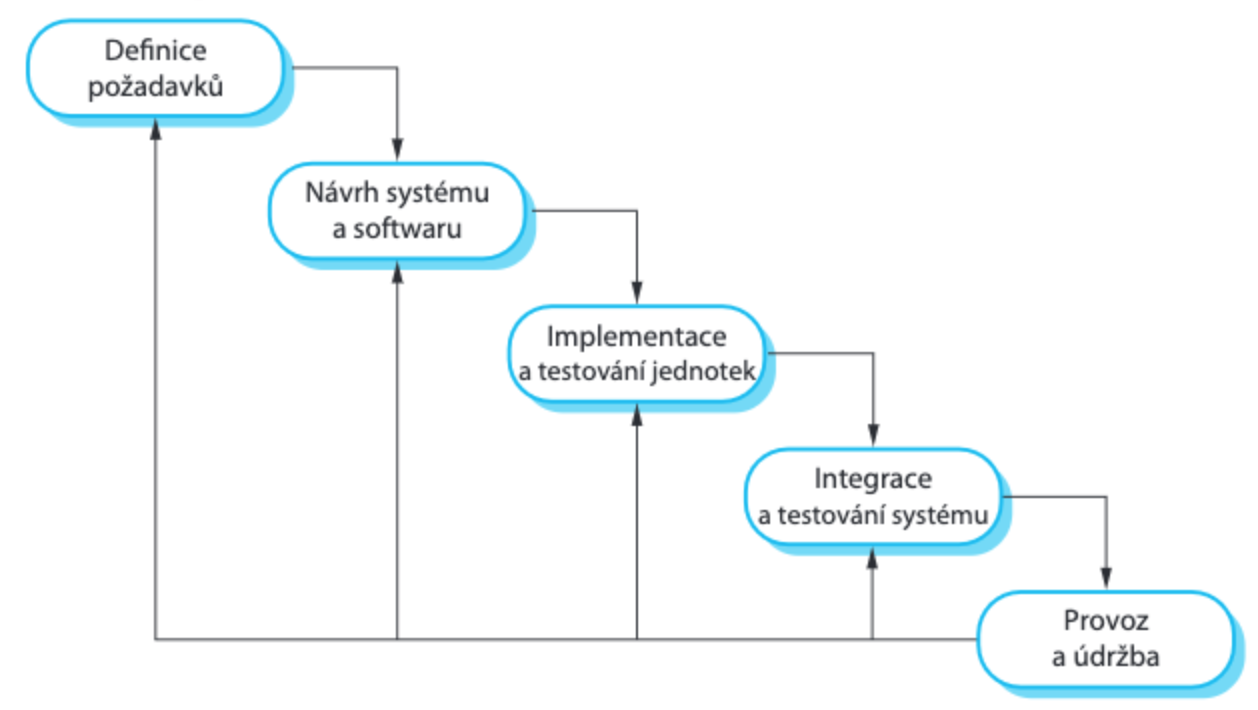
\includegraphics[width=1\textwidth]{Diplomka/Figures/waterfall.png}
    \caption{Vodopádový model (převzato z~\cite{ref:sommerrville_waterfall})}
    \label{fig:waterfall}
\end{figure}

Základní fáze vodopádového modelu vycházejí ze standardních potřeb vývoje softwaru:

\begin{enumerate}
\item \textit{Specifikace požadavků} -- na základě jednotlivých požadavků zákazníka jsou požadavky detailně sepsány a analyzovány.

\item \textit{Systémový a softwarový návrh} -- jednotlivé požadavky zákazníka určují náročnost na systém. Návrh zahrnuje také celkovou architekturu systému.

\item \textit{Implementace a unit testování} -- v~rámci této fáze se systém realizuje a každá jednotka je samostatně testována, zda splňuje určité požadavky.

\item \textit{Integrace a testování systému} -- jednotlivé vyvinuté části systému se integrují a otestují jako kompletní systém. Tím je zajištěno, že celý systém splňuje definované požadavky. Jakmile je produkt kompletně otestován, je předán zákazníkovi.

\item \textit{Provoz a údržba} -- během této fáze se systém nasazuje do ostrého prostředí. Dále v~rámci této fáze probíhá oprava chyb a vylepšování funkcí.

\end{enumerate}

V~praxi je složité jednotlivé fáze pečlivě oddělit a postupovat do další fáze pouze, jakmile je předchozí fáze plně dokončena. Proto se většinou jednotlivé fáze postupně překrývají a vyměňují si mezi sebou informace. Hlavní nevýhodou modelu je praktická nemožnost reagovat na měnící se požadavky zákazníka. Vodopádový model je vhodné zpravidla použít tam, kde víme, že se požadavky zásadně nebudou měnit.

\subsection{Rational Unified Process}
Rational Unified Process (RUP) je iterativní model vývoje softwaru vytvořený firmou Rational Software Corporation. RUP byl vytvořen a odvozen z~osvědčených praktik při vývoji softwaru. Mezi tyto praktiky například patří řízení změn, komponentová architektura, aktivní správa požadavků nebo například ověřování kvality software. Model obsahuje čtyři fáze, které se iterují dle potřeby. Jednotlivé fáze oproti vodopádovému modelu nesouvisejí s~technickými hledisky, ale soustředí se spíše na podniková hlediska. \cite{ref:rup_ibm_about} Fáze modelu RUP jsou následující:

\begin{enumerate}
\item \textit{Zahájení} -- cílem této fáze je vytvořit podnikový případ systému. V~rámci této fáze je potřeba identifikovat veškeré osoby a další systémy, které budou s~daným systémem pracovat či komunikovat.
\item \textit{Příprava} -- během této fáze se vytvoří architektura systému. Dále se vytvoří celkový plán projektu a identifikují se klíčová rizika, která mohou na projektu nastat. Během fáze vznikne například plán vývoje, UML diagramy nebo popis systému.
\item \textit{Konstrukce} -- tato fáze obsahuje návrh systému, samotné programování a testování, přičemž se zároveň jednotlivé části systému integrují. Dále během této fáze vzniká dokumentace. Na konci fáze je hotový funkční produkt připraven na dodání zákazníkovi.
\item \textit{Předávání} -- v~závěrečné fázi je funkční produkt spolu s~dokumentací předán zákazníkovi. Produkt je nasazen do ostrého prostředí a zprovozněn.
\end{enumerate}

U~modelu RUP je možno provádět inkrementaci samostatným opakováním jak jednotlivých fází, tak i celého procesu. Kromě čtyř fází RUP definuje jednotlivé disciplíny, jež jsou v~rámci fází prováděny. Velkou výhodou je, že tyto disciplíny nejsou navázány na jednotlivé fáze. Disciplíny jsou činnosti, prováděné během celého vývoje produktu. Disciplíny v~rámci modelu RUP jsou následující:

\begin{itemize}
\item Tvorba modelu,
\item správa požadavků,
\item analýza a návrh,
\item implementace,
\item testování,
\item nasazení,
\item správa konfigurace a změn,
\item řízení projektu,
\item správa prostředí.
\end{itemize}

Výše popsané fáze společně s~disciplínami je možno vidět na obrázku \ref{fig:rup}. Můžeme vidět, že různé disciplíny mají v~jednotlivých fázích vyšší důležitost než jiné.

\begin{figure}[!ht]
    \centering
    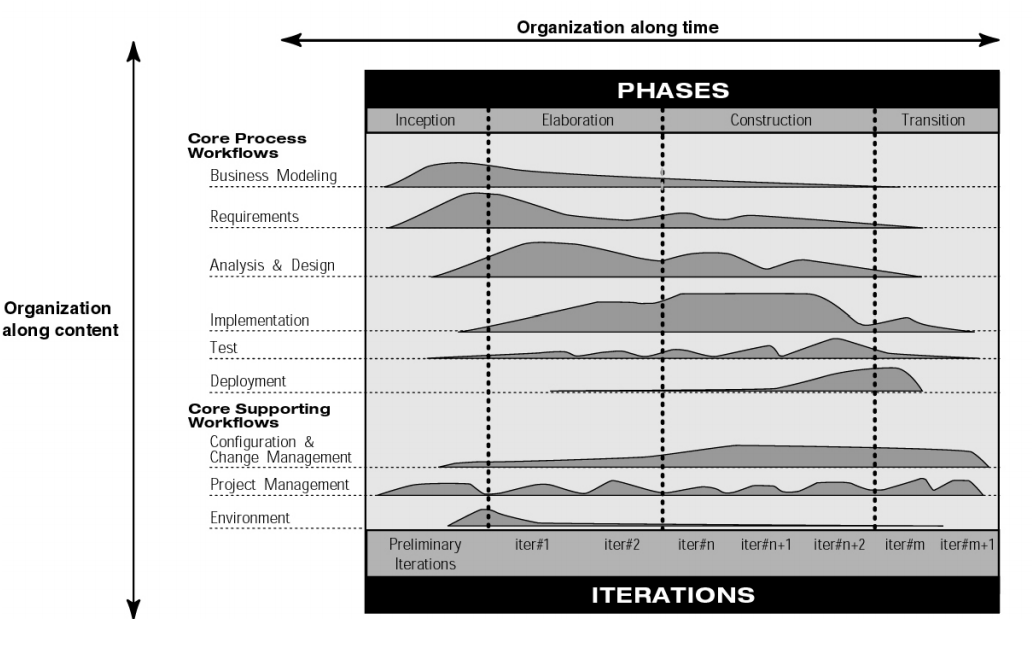
\includegraphics[width=0.75\textwidth]{Diplomka/Figures/rup.png}
    \caption{Grafické znázornění fází a disciplín RUP (převzato z~\cite{ref:rup_ibm})}
    \label{fig:rup}
\end{figure}

\section{Agilní metodiky vývoje}
Aktuální trh se softwarem se velmi rychle mění, a proto je potřeba aktivně reagovat na měnící se prostředí. Agilní přístupy patří k~inkrementálním způsobům vývoje. Software vytvářený pomocí vodopádového modelu může být v~době vydání již velmi zastaralý. Z~tohoto důvodu jsou agilní přístupy vývoje v~poslední době velmi oblíbené. Takto vyvíjený software je většinou dodán rychleji, ale zato může být dodán v~horší kvalitě. Takový přístup se ovšem nehodí u~kritických systémů, u~nichž je kladen velký důraz například na bezpečnost a spolehlivost. Software se během agilního vývoje vytváří ve verzích, kdy každá nová verze obsahuje nové funkcionality. Jednotlivé vývojové procesy se prolínají a většinou neexistuje podrobná specifikace a dokumentace systému. V~dokumentaci obvykle bývají pouze základní a nejdůležitější prvky systému. Tento nedostatek se ovšem může rychle vymstít při následné údržbě daného softwaru.

Filozofie agilních metodik vychází z~manifestu, na němž se shodli vývojáři těchto vývojových metod. Manifest popisuje čtyři základní hodnoty, jichž si autoři cení \cite{ref:agilne_manifesto}:

\begin{itemize}
\item Jednotlivci a interakce před procesy a nástroji.
\item Fungující software před vyčerpávající dokumentací.
\item Spolupráce se zákazníkem před vyjednáváním o~smlouvě.
\item Reagování na změny před dodržováním plánu.
\end{itemize}

Každý vývojový proces má svá pozitiva a svá negativa. Mezi pozitiva při agilním vývoji patří například rychlejší vývoj, větší flexibilita vývoje, kdy je možno upravovat směr dalšího vývoje dle potřeby zákazníka nebo například zapojení zákazníka do procesu vývoje. Mezi negativa patří nekompletní dokumentace, závislost na vývojovém týmu, kdy při rozpadu týmu může dojít k~problémům. Dalším problém může být, že v~dnešní době chce každá firma vyvíjet agilně, i když na to není personál proškolený a nikdo z~dané firmy pořádně neví, co to znamená agilní vývoj.

Podle Iana Sommervilla \cite{ref:sommerrville_agile_products} jsou agilní metody úspěšné pouze pro určité typy softwarových systémů:

\begin{enumerate}
\item Vývoj malého nebo středně velkého systému, který je určen k~prodeji.
\item Vývoj systémů pro zákazníka, kde si zákazník uvědomuje nutnost zapojit se do procesu vývoje a kde neexistuje mnoho pravidel, která mají vliv na vývoj softwaru.
\end{enumerate}


\subsection{Extrémní programování}
Dle Kenta Becka \cite{ref:what_is_xp} je extrémní programování agilní metoda, která spočívá ve změně myšlení a zvyků při vývoji. Extrémní programování se zaměřuje na excelentní programovací schopnosti, zlepšení komunikace mezi členy týmu a týmovou práci. Extrémní programování se zaměřuje na zextrémnění a zefektivnění těch úkonů, které se při vývoji osvědčily. Je důležité z~extrémního programování do procesu zařadit pouze ty aktivity, které mají hodnotu pro vývojový tým a přinášejí benefit zákazníkovi. Můžeme zde například zařadit párové programování, kdy dva programátoři vyvíjejí společně jednu funkčnost, přičemž jeden programátor pozoruje druhého při programování. Tyto role se pravidelně střídají. Nevýhodou tohoto přístupu je, že takto vyvíjený software zabere více placeného času. Výhoda spočívá naopak v~tom, že software obsahuje méně chyb díky vzájemné revizi kódu.

Další obor, který může být pomocí extrémního programování řešen je extrémnější testování softwaru, kdy samotní programátoři programují jednotkové (unit) testy, ale zároveň testuje také zákazník pomocí akceptačních testů. Extrémní programování takto řeší prakticky každou oblast vývoje, která se při vývoji osvědčila a může být zefektivněna. Jednotlivá zadání úkolů jsou řešena stejně jako v~metodě Scrum pomocí uživatelských příběhů (takzvané \textit{User stories}). Dalšími možnými praktikami, jež extrémní programování řeší, jsou například přítomnost zákazníka na pracovišti, vydávání malých verzí softwaru, průběžná integrace anebo neustálá refaktorizace kódu.

\subsection{Scrum}
Dle Josefa Myslína \cite{ref:scrum_myslin} je to agilní technika, při které se více než technické procesy řeší projektové procesy. Vymysleli ji Ken Schwaber a Jeff Sutherland na začátku 90. let 20. století. Týmy, které ve Srumu pracují, jsou samoorganizované, přičemž vývojový tým nemá přímého nadřízeného. Tým obsahuje několik klíčových rolí, mezi něž patří \textit{Product owner} (vlastník produktu), který komunikuje se zákazníkem a případně řeší priority ve vykonané práci. Dále se zde vyskytuje \textit{Scrum master}, který má na starost samotný proces a interakci s~týmem. Samozřejmostí je samotný vývojový tým. Scrum stojí na třech základních pilířích:

\begin{enumerate}
\item \textit{Transparentnost} -- všichni v~týmu by měli mít přehled o~veškerém dění v~rámci projektu. Každý člen týmu tedy například ví, v~jakém stavu je určitý úkol a proč existuje.
\item \textit{Kontrola} -- pravidelně se v~rámci celého týmu dělá kontrola, zda procesy a fungování týmu jsou vyhovující.
\item \textit{Adaptace} -- na základě zjištěných požadavků v~rámci pravidelných kontrol se provádějí změny, aby byl daný tým spokojený a doručoval dále vynikající výsledky.
\end{enumerate}

Veškerý vývoj produktu probíhá v~pravidelných iteracích, které jsou nazývány \textit{Sprinty}. Tyto iterace mají nejčastěji trvání od dvou týdnů po jeden měsíc. Na konci každého sprintu je dodána nová verze funkčního systému.

Jak je možno vidět na obrázku, \ref{fig:scrum_cyklus} na začátku každého sprintu probíhá seznámení s~úkoly na daný sprint a plánování, které úkoly musí tým daný sprint doručit. Během sprintu probíhají různé druhy schůzek. Každý den probíhá rychlá schůzka nazývaná \textit{Standup}, během níž členové týmu v~rychlosti představí, co budou daný den řešit a co řešili předešlý den. Na konci každého sprintu probíhá pravidelná kontrola, jež se nazývá retrospektiva, a dále samotné zhodnocení sprintu. Na této schůzce je řešeno, jaké adaptace by měl tým provést, aby následující sprint proběhl lépe.

\begin{figure}[!ht]
    \centering
    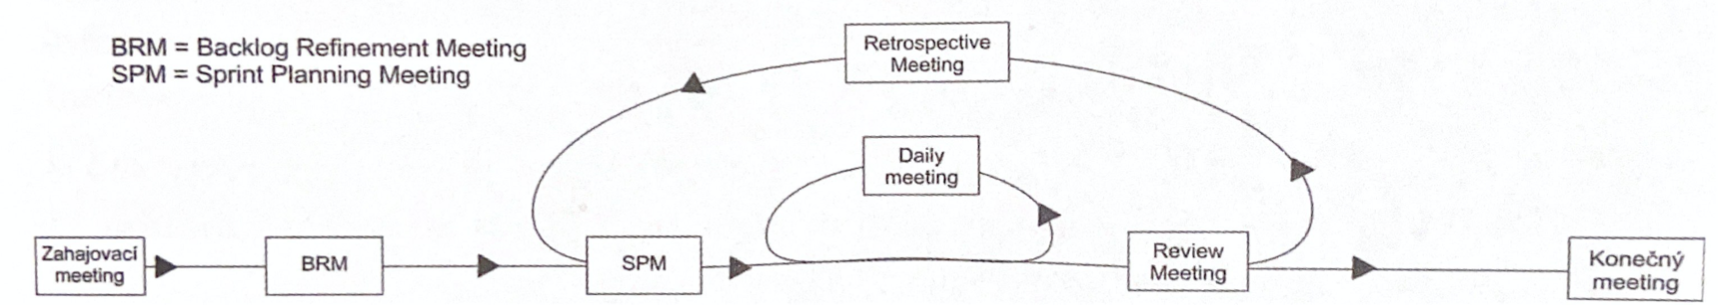
\includegraphics[width=1\textwidth]{Diplomka/Figures/scrum.png}
    \caption{Vývojový cyklus řízený pomocí metodiky Scrum (převzato z~\cite{ref:scrum_myslin_cyklus_img})}
    \label{fig:scrum_cyklus}
\end{figure}

Jednotlivé schůzky by se poté daly rozdělit do tří základních skupin:

\begin{itemize}
\item \textit{Plánovací} -- tento typ schůzek předchází jakékoli aktivitě, která po schůzce probíhá. Během těchto schůzek může být plánován buď celý projekt, nebo je naplánován sprint.
\item \textit{Hodnotící} -- tyto schůzky probíhají buď na konci sprintu, nebo na konci projektu. Během tohoto typu schůzek se hodnotí, zda to, co proběhlo, proběhlo v~pořádku, a případně co bylo špatně.
\item \textit{Plánovací i hodnotící} -- do této skupiny spadá pouze denní schůzka zvaná \textit{Standup}. Během schůzky se hodnotí předchozí den a plánuje se, co se bude dále daný den dělat. Během schůzky mají všichni členové týmu možnost vidět, jak se úkol vyvíjí, a zda úkol na něco nečeká.
\end{itemize}


Jednotlivá zadání úkolů jsou psána pomocí uživatelských příběhů (takzvané \textit{User stories}), přičemž většinou obsahují jen minimum technických informací. Jednotlivé uživatelské příběhy nepopisují technickou interakci ze systémem. Uživatelské příběhy mají  sjednocenou podobu například ve tvaru: \uv{Jako \textit{role} chci \textit{cíl} tak, aby \textit{užitek}.} Tedy například: \uv{Jako uživatel chci vidět seznam zboží v~objednávce tak, aby si uživatel mohl zboží zkontrolovat.} \cite{ref:scrum_myslin_us}

\section{V-Model}
V-model je grafické znázornění vývojového cyklu používaného prakticky u~jakéhokoli vývoje, u~něhož je důležité nepřetržité fungování a bezchybnost systému. Model je tedy využíván prakticky v~každém odvětví, nejen v~automobilovém průmyslu nebo softwarovém vývoji kritických systémů. Tento model zdědil po vodopádovém modelu jistou kaskádovitost, kdy každý krok je proveden až po předchozím kroku. Za rozdílnost V-Modelu lze považovat to, že je oproti agilním přístupům zaměřen na velmi důkladnou kontrolu a testování systému. Kontrola a testování probíhá již v~počátečních etapách návrhu systému. Jednotlivé testování systému se provádí ve stejné době jako určitá část vývoje. Tedy například jednotkové testy se píšou během implementační části nebo například integrační testování probíhá při integraci jednotlivých komponent systému. Je vhodný zejména pro projekty, kde je většina požadavků jasná a předem daná. Grafické znázornění V-Modelu je možno vidět na obrázku \ref{fig:v_model}.

V-Model je graficky definován do tvaru velkého písmene V. Na levé straně modelu se nachází fáze spojené s~verifikací. První fází v~rámci verifikační části je sběr požadavků, v~němž jsou od zákazníka získány požadavky. Tyto požadavky jsou následně analyzovány. V~další fázi se provede na základě těchto nasbíraných požadavků návrh systému. Dále následuje vytvoření architektury systému a návrh jednotlivých modulů. Poté je na základě veškeré analýzy provedena implementace.

Na pravé straně jsou fáze validační, v~nichž se produkt testuje a validuje se jeho funkčnost. Jednotlivé fáze jsou vzájemně propojeny. V~nejnižší vrstvě probíhá jednotkové testování, jež testuje chování malých modulů. Dále probíhá integrační testování, jež je prováděno proti návrhu architektury. Jakmile je úspěšně provedeno integrační testování, je testován návrh systému systémovými testy. Na nejvyšší úrovní probíhá akceptační testování, jež ověřuje, zda jsou správně implementovány veškeré definované požadavky zákazníka. Každý přechod do jiné fáze probíhá, jakmile je kompletně splněna předchozí fáze.

 \begin{figure}[!ht]
    \centering
    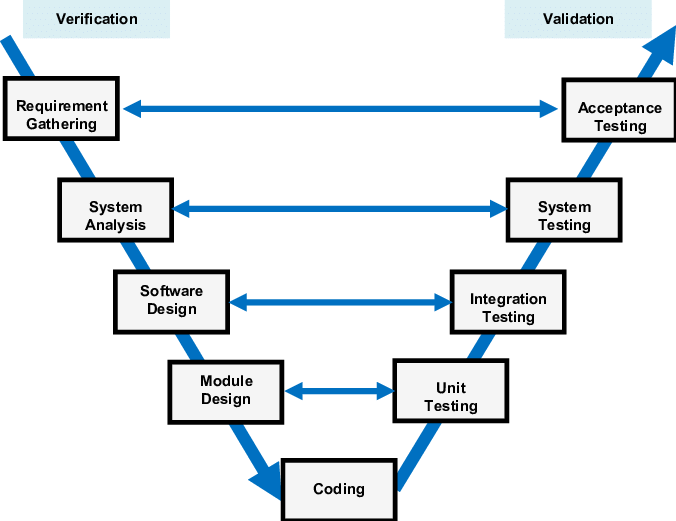
\includegraphics[width=0.7\textwidth]{Diplomka/Figures/v-model-in-software-testing.png}
    \caption{Grafické znázornění V-Modelu (převzato z~\cite{ref:vmodel_Tierno2016})}
    \label{fig:v_model}
\end{figure}


\chapter{Metriky}
\label{sec:metrics}
Jelikož v~rámci praktické části vytvářím nástroj pro vytváření metrik, je nutno se nejprve seznámit se samotnou teorií metrik a měření vývoje. Metriky se mohou používat nejen při samotném sběru požadavků, ale i při vývoji systému. Během sběru požadavků a vývoje celého systému je potřeba dodržovat určité standardy. V~automobilovém průmyslu je to nejčastěji standard Automotive SPICE, který je podrobněji popsán v~kapitole \ref{sec:aspice}. Pro to, aby bylo zajištěno plnění definovaného standardu a plnění jednotlivých úkolů pro dokončení projektu, je využíváno právě metrik.

Dle výkladu Iana Sommervilla \cite{ref:metric_definition} je metrika softwaru vlastnost softwarového systému, systémové dokumentace nebo vývojového procesu, kterou lze objektivně měřit. Mezi typické obecné metriky můžeme zařadit například počet řádků kódu, počet splněných požadavků z~celkového počtu zadaných, počet nalezených chyb v~softwaru a další. Management mohou ovlivnit jak kontrolní, tak i prediktivní metriky. Při změně provedené na základě kontrolní metriky je změněn samotný softwarový proces. Pokud manažer provede rozhodnutí pro změnu v~procesu, mohou prediktivní metriky usnadnit odhad, jak bude změna náročná na provedení změn.

Při měření vývoje softwaru pomocí metrik se snažíme odvodit numerické hodnoty nebo profil atributu vývoje daného softwaru, části systému nebo dokonce i samotného procesu. Na základě naměřených údajů pomocí metrik dokážeme zjistit, jak je standard dodržován nebo jakým směrem se vývoj ubírá. Dále na základě těchto údajů dokážeme také zjistit kvalitu vyvíjeného systému nebo softwaru a také dokážeme hodnotit efektivitu jednotlivých procesů, které se při vývoji používají. Pomocí metrik také můžeme zjistit, zda používané nástroje a metody přispívají k~lepší efektivitě práce či nikoli.

Při zavádění nového nástroje v~rámci organizace můžeme využít metriky tak, že část daného vývoje změříme metrikami před zavedením nástroje. Po určité definované době od zavedení nástroje pomocí metrik změříme znovu stejnou část vývojového procesu a vyhodnotíme, zda je tým při vývoji efektivnější než před prvním měřením. Pod tímto si můžeme například představit zavedení nového nástroje na automatické testování vyvíjeného softwaru. Před zavedením pomocí metrik zjistíme, kolik se v~softwaru vyskytuje chyb, a poté tyto údaje porovnáme s~údaji naměřenými po zavedení nástroje. Takto získaná data můžeme tedy používat pro zlepšení samotného vývoje a procesů.

Jedním ze základních dělení metrik je dělení na \textbf{kontrolní} a prediktivní metriky. Kontrolní metriky, jak již vyplývá ze samotného názvu, slouží pro správu a kontrolu prováděných procesů. Typickými metrikami patřícími mezi kontrolní metriky jsou počet nahlášených chyb během vývoje, průměrný čas strávený na opravě detekovaných chyb, počet splněných úkolů od zahájení vývoje a mnoho dalších. Mezi prediktivní metriky řadíme metriky, které předpovídají vlastnosti vyvíjeného produktu nebo softwaru. Typickými představiteli jsou například cyklomatická složitost určité komponenty, počet tříd nebo databázových tabulek. Prediktivní metriky, které souvisejí s~vlastnostmi vyvíjeného produktu nebo softwaru, se mohou označovat také jako produktové metriky. \cite{ref:metric_definition}

\section{Kontrolní metriky}
Tyto metriky slouží jako statistické údaje pro kontrolu daného softwarového procesu. Můžeme zde zařadit údaje o~času stráveném na nějakém konkrétním úkolu. Vysledovaná a naměřená data poté slouží jako podklad ke zlepšování osobního a softwarového procesu.

Podle Iana Sommervilla \cite{ref:kontrolni_metriky} lze shromažďovat tři typy kontrolních metrik:

\begin{enumerate}
\item \textit{Zbývající čas, který je potřebný k~dokončení definovaného procesu} -- v~rámci této kategorie můžeme zařadit měření zbývajícího času k~dokončení procesu, čas strávený testováním systému a další. V~rámci této kategorie dokážeme určit efektivitu daného procesu. Z~naměřených hodnot tedy dokážeme zjistit, zda se efektivita zvýšila nebo snížila.

\item \textit{Prostředky, které jsou nutné pro dokončení definovaného procesu} -- můžeme měřit například počet potřebných programátorů k~dokončení určitého procesu, náklady spojené s~vývojem systému a další. V~této kategorii také dokážeme měřit efektivitu procesu, například zda potřebné zdroje k~dosažení výsledku klesají či nikoli.

\item \textit{Počet zjištěných výskytů definované události} -- měříme a monitorujeme počet určitých vzniklých událostí, které mohou přímo nebo nepřímo ovlivňovat určitý proces. Můžeme zde uvést například počet nalezených chyb při testování, počet změněných požadavků, počet řádků kódu pro jeden požadavek a mnoho dalšího.

\end{enumerate}

V~rámci kontrolních metrik můžeme tedy zjistit efektivitu samotného vývoje a lépe odhadnout směr vývoje procesu. Pomocí metrik můžeme měřit potřebný čas a úsilí k~dokončení,nebo posunu procesu. Například pomocí monitorování počtu vad dokážeme odhadnout kvalitu výsledného systému. Tedy při zvýšení počtu vad můžeme předpokládat, že v~systému byla nalezena většina chyb a systém bude tedy v~produkčním prostředí stabilní a kvalitní. Je důležité zjistit, které informace je nutno pro následné zlepšení procesu a také systému sledovat, měřit a shromažďovat.

\section{Prediktivní metriky}
Jak již bylo zmíněno, jde o~metriky, které předpovídají vlastnosti výsledného produktu. Mezi prediktivní metriky můžeme zařadit produktové metriky, pomocí nichž dokážeme měřit interní atributy vyvíjeného produktu případně softwaru. Interní atributy si můžeme představit například jako konkrétní vlastnosti vyvíjeného softwaru. Jde tedy o~velikost softwaru, počet naprogramovaných tříd, počet uživatelských obrazovek a mnoho dalšího. Tyto vlastnosti nemusí mít přímou spojitost se zjištěním kvality softwaru, ale mohou sloužit jen jako informativní hodnota pro manažery k~odhadu velikosti.

Produktové metriky lze dále dělit na dvě základní třídy podle původu měření. První třídou jsou statické metriky, které získávají data pomocí měření reprezentace systému -- dokumentace systému, návrh systému a samotný program. Můžeme zde zařadit počet tříd, počet formulářů, průměrnou délku tříd a další. Tyto metriky nám dokážou usnadnit hodnocení a odhad složitosti a komplexnosti celého softwaru. Zároveň nám mohou být tyto informace užitečné pro přípravu na následnou údržbu celého systému.

Druhou třídou produktových metrik jsou dynamické metriky, pro které se data shromažďují průběžně pomocí spuštěného systému při testování nebo na produkčním prostředí. Tyto metriky nám pomáhají hodnotit celkovou spolehlivost systému v~produkčním prostředí. Dále z~těchto metrik můžeme odhadnout či zjistit náročnost a efektivitu systému pro produkční prostředí. Mezi dynamické metriky řadíme metriky měřící počet nedodělaných scénářů objevených testováním, počet nefunkčních požadavků nebo také informace o~maximálním možné zatížení systému.

\section{Reprezentace a vizualizace metrik}
\label{sec:visualisation}
Metriku si můžeme představit jako sled čísel, která nám slouží coby ukazatele stavu procesu. Metriky můžeme tedy reprezentovat tak, abychom dokázali určit stav daného procesu nebo vyvíjeného systému. Pomocí metriky se může manažer rozhodovat o~krocích, které budou podniknuty, aby byl proces efektivní a aby byl systém vytvořen v~definované kvalitě a času. Nejčastěji si metriku můžeme představit jako tabulku a nebo pomocí grafické vizualizace, která vychází z~dat tabulky.


\subsection{Zobrazení pomocí tabulky}
Každou metriku si můžeme představit jako tabulku dat nasbíraných během procesu. Je to tedy základní vizualizace nasbíraných surových dat. Nevýhodou tabulkového zobrazení je to, že při některých metrikách je složité a náročné si představit, co daná čísla reprezentují a zda číslo, které vidíme, je dobré nebo špatné. Většinou se proto zobrazení tabulky kombinuje s~grafem, pomocí něhož můžeme lépe pochopit daný kontext měřené veličiny.

\subsection{Vizualizace grafem}
Vizualizace pomocí grafu bývá jednou z~nejčastějších možností, jak metriku zobrazit a následně jednoduše pochopit. Pro kýženou vizualizaci grafem můžeme použít několik typů grafů. Vizualizace většinou vychází buď přímo ze surových dat, nebo z~připravených dat používaných pro zobrazení v~tabulce. Pro vizualizaci dat je možno použít prostředky z~několika stovek různých frameworků, které graf vytvoří a vizualizuje. Mezi nejčastěji používané typy grafů patří různé variace sloupcového, spojnicového a koláčového grafu. V~rámci IBM Jazz a aplikací, které jsou naprogramovány pomocí jazyka Java, můžeme nalézt použitý framewrok BIRT, kterému se věnuji v~rámci kapitoly \ref{sec:birt}. Druhou možností vizualizace grafu na webových stránkách je pomocí JavaScriptové knihovny. V~rámci této práce porovnávám tři JavaScriptové knihovny s~názvem Google Charts, amCharts a Chart.js v~kapitolách \ref{sec:google_charts}, \ref{sec:amcharts} a \ref{sec:chartjs}.

\subsection{BIRT}
\label{sec:birt}
BIRT je open source softwarový projekt vyvíjený konsorciem Eclipse Foundation a původně sponzorovaný společností Actuate s~pomocí společnosti IBM, který poskytuje platformu pro vytváření a vizualizaci dat. Je určený zejména pro webové a klientské aplikace, které jsou založeny na prostředí Java a Java EE. BIRT se skládá ze dvou hlavních komponent \cite{ref:birt_about}:

\begin{itemize}
\item vizuální návrhář sestav v~IDE Eclipse,
\item komponenta pro generování navržených sestav, které lze nasadit do libovolného Java prostředí.
\end{itemize}

Projekt BIRT také obsahuje mapovací modul, který je plně integrován do návrháře sestav a může být použit samostatně k~integraci grafů do aplikace. Pomocí technologie BIRT je výstupy možno generovat kromě grafů ve formátu SVG také jako seznamy dat (například pomocí tabulky) nebo jako textové dokumenty. Sestavy BIRT se skládají ze čtyř hlavních částí \cite{ref:birt_about}:

\begin{itemize}
\item \textit{Data} -- poskytuje podporu pro přístup k~datům pomocí JDBC, XML, webových služeb prostých databázových souborů. Vytvořená sestava může dále zobrazovat data z~libovolného počtu zdrojů dat. BIRT využívá ODA (Open Data Access), který umožňuje komukoli vytvořit novou sestavu pro jakýkoli druh tabulkových dat.
\item \textit{Transformace dat} -- vygenerované sestavy reprezentují seřazená, filtrovaná a seskupená data podle definovaných potřeb uživatele. Tato data jsou poté připravena pro vizualizaci.
\item \textit{Obchodní logika} -- jelikož jsou data v~reálném světě málokdy strukturována přesně tak, aby vyhovovala z~byznysového hlediska pro jednotlivé sestavy, je nutno je nejprve strukturovat tak, aby pro transformaci a vizualizaci vyhovovala. Tato strukturalizace je možná buď přímo pomocí BIRT v~jazyce JavaScript, nebo externě pomocí zdrojového kódu v~programovacím jazyku Java.

\item \textit{Vizualizace} -- Jakmile jsou data pro vizualizaci připravena, je možno je vizualizovat například pomocí grafů nebo tabulek. Jedna připravená sada dat může být vizualizována více způsoby.
\end{itemize}

Architektura BIRT se skládá z~\textit{Report Designeru}, který zajišťuje vytváření reportů, jež vygeneruje do formátu XML. Dále se skládá z~\textit{Report enginu}, který vygeneruje jednotlivé vizualizace dat do definovaných formátů, například PDF, HTML, Excel, Word a další. Celkovou architekturu systému BIRT je možno vidět na obrázku \ref{fig:birtarch}.

\begin{figure}[!ht]
    \centering
    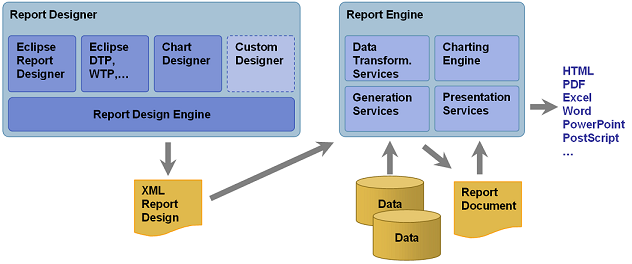
\includegraphics[width=0.8\textwidth]{Diplomka/Figures/birtarch.png}
    \caption{Architektura BIRT (převzato z~\cite{ref:birt_about})}
    \label{fig:birtarch}
\end{figure}
\subsection{Metabase}
Podobně jako BIRT je Metabase možno použít jako nástroj pro zobrazování a vizualizaci neagregovaných dat. Je to moderní aplikace, kterou je možno spustit pomocí virtualizace Docker. Grafy je možno vytvářet a skládat pomocí SQL dotazů. Aplikace je poskytována jak zdarma, tak i za poplatek v~případě hostování v~cloudu nebo jako \textit{Enterprise} licence pro velké společnosti. Aplikaci je také možno použít jako celý \textit{Business intelligence}. Metabase je možno napojit na velké množství typů databází včetně MySQL, MongoDB, Oracle a dalších. Výstupní zprávy dokáže posílat také pomocí zpráv v~aplikaci Slack. Není to tedy pouze knihovna sloužící pro vykreslení grafů, ale kompletní řešení. \cite{ref:metabase}


\subsection{Google Charts}
\label{sec:google_charts}
Je to veřejně dostupná interaktivní webová služba, která dokáže vytvořit grafy z~poskytnutých dat. Knihovna je vyvinutá společností Google a je zcela bezplatná. Velkou výhodou knihovny je, že je plně přizpůsobitelná a funguje pomocí HTML5 a SVG. Zobrazení grafů je tedy kompatibilní na všech zařízeních včetně mobilních telefonů a tabletů. Další výhodou je velká variace různých typů grafů, které mohou být zobrazovány dynamicky a při zobrazení měněny a lehce upravovány. Velkou nevýhodou je, že grafy nejsou plně interaktivní a není možno je za běhu bez nutnosti obnovení stránky měnit a jednoduše filtrovat. Oproti BIRT (viz kapitola \ref{sec:birt}) knihovna poskytuje pouze vizualizaci poskytnutých agregovaných dat.

Služba funguje jako JavaScriptová knihovna. Uživatel tedy dodá data pro JavaScript, který potřebný graf následně vykreslí. Služba vychází z~původní Google Chart API, která fungovala čistě pomocí HTTP metod a není kompatibilní s~aktuálním Google Charts. \cite{ref:google_charts}

\subsection{amCharts}
\label{sec:amcharts}
Je to jedna z~mnoha knihoven fungujících na jazyce JavaScript pro vykreslování grafů na webových stránkách. Samotná knihovna je vytvořena v~jazyce TypeScript. Vykreslování probíhá pomocí dynamického zobrazování SVG obrázků, které jsou plně kompatibilní jak s~ovládáním pomocí myši, tak pomocí dotyků na mobilních zařízeních. Knihovna nepoužívá žádné jiné knihovny třetích stran a podporuje konfiguraci jak pomocí objektů v~TypeScriptu nebo JavaScriptu, tak pomocí univerzálního JSONu. Knihovna obsahuje obrovské množství různých typů grafů a jejich variací. Kromě klasických grafů nabízí také mapy, rozmanité diagramy a další variace různých typů grafů. Jednotlivé grafy je možno jakkoli upravovat dle vlastního uvážení včetně typu písma a dalších vlastností. Grafy v~amCharts vypadají moderně, obsahují mnoho volitelných animací a různě barevné šablony.  V~základu také nabízí manipulaci s~daty, která je možno skrývat či zobrazovat. Knihovna je v~základní verzi se zobrazením loga v~rohu každého grafu zdarma, pro odstranění loga je nutno zaplatit licenci. Podobně jako u~služby Google Charts je nutno dodat data již připravená a agregovaná. \cite{ref:amcharts_web}

\subsection{Chart.js}
\label{sec:chartjs}
Chart.js je jednoduchá knihovna určená pro zobrazování grafů na webových stránkách. Knihovnu je možno získat plně zdarma a je dostupná jako otevřený software. Nabízí osm typů grafů, které mohou být animované a přizpůsobitelné. Grafy jsou generovány pomocí HTML5 Canvas a jsou tedy dostupné ve všech novějších prohlížečích. Komponenta je plně responzivní a je tedy možno ji použít na všechna možná zařízení. Nevýhodou je příliš velká jednoduchost a omezenost, která je však vykoupena rychlým nasazením do již existujících webových stránek. \cite{ref:chartjs}



\chapter{Automotive SPICE}
\label{sec:aspice}
Automotive Software Process Improvement and Capability Determination (zkráceně ASPICE) je standard, používaný v~automobilovém průmyslu pro vývoj mechatronických a softwarových systémů v~automobilovém průmyslu. Vychází z~obecného standardu SPICE (ISO/IEC 15504), který se věnuje obecnému vývoji softwaru. Od vytvoření v~roce 2005 je Automotive SPICE oborovou variantou této normy. Standard je volně přístupný na webových stránkách v~několika světových jazycích \cite{ref:aspice_download_obecne}. Poslední dostupná verze je verze 3.1 z~roku 2017. Tato verze obsahuje opravu drobných jazykových chyb a vychází z~verze 3.0 \cite{ref:aspice_download_verze}.

Standard Automotive SPICE byl vyvinut v~rámci spolupráce evropských automobilových společností. Ty se spojily do sdružení Automotive Special Interest Group (SIG). Dále je standard aktualizován skupinou Quality Management Center in the German Association of Automotive Industry (VDA QMC). Standard je tímto sdružením pravidelně aktualizován a upravován, aby vyhovoval nejnovějším požadavkům. Mezi evropské automobilky zapojené do sdružení SIG patří například:

\begin{itemize}
  \item BMW Group,
  \item Daimler AG,
  \item Jaguar,
  \item Volkswagen AG,
  \item Volvo Car Corporation a další.
\end{itemize}

V~současné době se automobily skládají z~velkého množství součástí. Automobily se tedy již neskládají pouze z~mechanických součástí. V~poslední době roste množství používaného softwaru nejen při vývoji, ale i v~samotných automobilech. Většina softwaru v~automobilu slouží  pro zajištění nejen bezpečnostních funkcí, ale také pro zajištění životně důležitých funkcí automobilu včetně brzd a samotného řízení. Nesmí se tedy stát, že software v~automobilu selže a například zablokuje brzdy a způsobí havárii. Dodržování tohoto standardu je rozhodující kritériem při volbě dodavatelů dané automobilové společnosti, jelikož zajišťuje, že dodavatel splňuje určité standardy vývoje.

V~rámci vývoje v~automobilovém průmyslu je většina systémů vyvíjena pomocí V-Modelu. Každá část  vývojového procesu musí mít definovány cíle. Aby bylo možno určit, zda jsou cíle splněny, jsou používány metriky (viz kapitola \ref{sec:metrics}).

\section{Referenční procesní model}
Je to jeden z~procesních modelů v~rámci standardu Automotive SPICE.
Každý proces obsahuje kromě popisu také funkční cíle v~daném prostředí a seznam výsledků a výstupů, jichž má proces dosáhnout.
%Každý proces  je popsán v podmínkách prohlášení o účelu. Prohlášení o účelu obsahuje jedinečné funkční cíle procesu při provádění v konkrétním prostředí. Ke každému prohlášení o účelu je přidružen seznam konkrétních výsledků jako seznam očekávaných pozitivních výsledků výkonu procesu.
%Each process is described in terms of a purpose statement. The purpose statement contains the unique functional objectives of the process when performed in a particular environment. For each purpose statement a list of specific outcomes is associated, as a list of expected positive results of the process performance.
\cite{ref:aspice_download_procesni_modely}


Referenční procesní model definuje několik procesů ve třech základních kategoriích:

\begin{itemize}

\item primární procesy,
\item podpůrné procesy,
\item organizační procesy.

\end{itemize}

Jednotlivé kategorie procesů a samotné procesy jsou detailně probrány v~kapitole \ref{sec:aspice_processes} a je možno je graficky seskupené vidět na obrázku \ref{fig:prm}.
\begin{figure}[!ht]
    \centering
    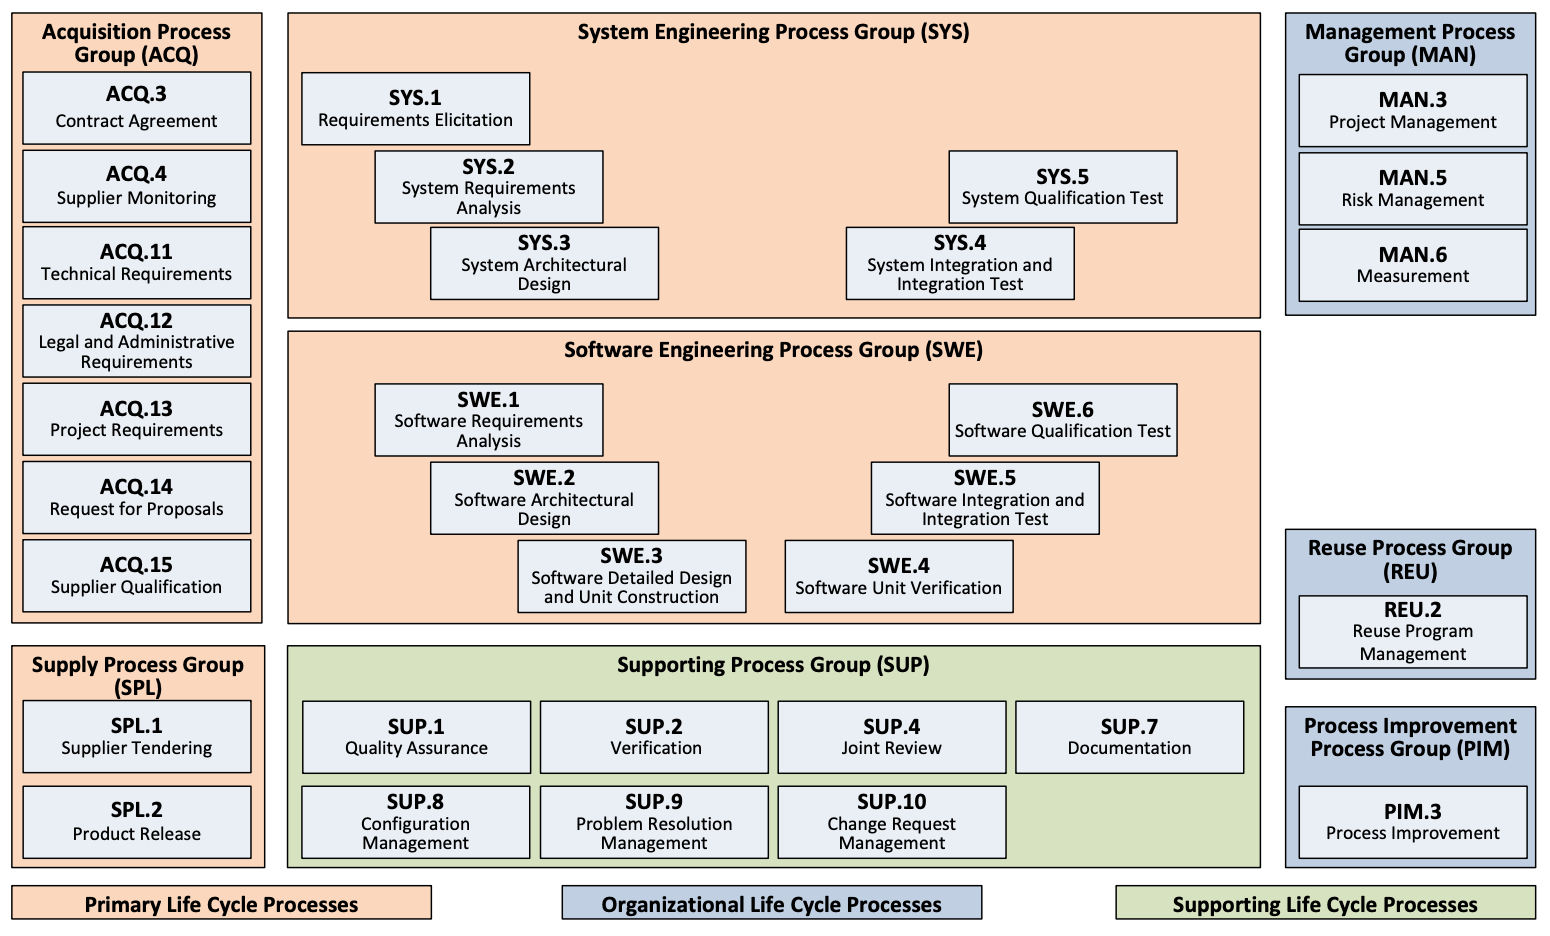
\includegraphics[width=1\textwidth]{Diplomka/Figures/prm.png}
    \caption{Referenční procesní model (převzato z~\cite{ref:aspice_download_prm})}
    \label{fig:prm}
\end{figure}


% ) a je určen pro provádění hodnocení schopnosti používání tohoto softwarového procesu dodavatelem pro automobilový průmysl.
% V rámci ASPICE existují dva druhy procesních modelů. První z nich je model hodnocení procesů (PAM), který byl vyvinut v souladu se standardem ISO/IEC 33004. Tento procesní model obsahuje několik hodnotících ukazatelů

% PAM [3, str. 10] obsahuje sadu hodnotících ukazatelů výkonnosti a způsobilosti procesů. Tyto indikátory jsou základem pro shromažďování objektivních důkazů, které model umožňuje s posuzováním přiřadit hodnocení. Dále PAM definuje dvoudimenzionální model způsobilosti procesu. V první dimenzi proces jsou procesy definovány a rozděleny do kategorií procesů, kde v rámci kategorie procesů jsou procesy seskupeny do skupin procesů v druhém stupni v souladu se zabývanou druhou činností. V druhé dimenzi schopnost je definován soubor atributů procesu seskupených do úrovně schopností. Atributy procesu poskytují měřitelné vlastnosti způsobilosti procesu. Ještě dodáváme, že [4, str. 8] PAM poskytuje další ukazatele výkonnosti a způsobilosti procesů přizpůsobených potřebám k provádění posouzení softwarového procesu schopnosti dodavatelů pro automobilový průmysl.



%Druhý procesní model je procesní referenční model (PRM). Ten se používá ve spojení s modelem hodnocení procesu při provádění hodnocení dané společnosti.
% \cite{ref:aspice_download_procesni_modely}

\section{Procesy Automotive SPICE}
\label{sec:aspice_processes}
V~rámci každé základní kategorie procesů existují v~referenčním procesním modelu podkategorie procesů podle toho, jakým okruhem činností se zaobírají. Procesy jsou pojmenovány pomocí třímístného identifikátoru, který určuje podkategorii procesu. Dále název procesu obsahuje číslo, které identifikuje proces v~rámci své podkategorie.

\subsection{Primární procesy}
Kategorie primárních procesů životního cyklu sestává z~procesů, které mohou být použity zákazníkem při získávání produktů od dodavatele a dodavatelem při reakci a dodávce produktů zákazníkovi, včetně technických procesů potřebných pro specifikaci, návrh, vývoj, integraci a testování.

Mezi první podkategorii primárních procesů patří akviziční procesy. Do této podkategorie patří procesy, jež jsou prováděny zákazníkem případně dodavatelem, který je v~roli zákazníka požadujícího službu nebo produkt. Tato podkategorie akvizičních procesů obsahuje sedm procesů:

\begin{itemize}
\item ACQ.3 -- Dohoda o~smlouvě. Během tohoto procesu probíhá dohoda o~samotné smlouvě a schválení smlouvy. Po úspěšném dokončení procesu je dohodnutá smlouva podepsána a odsouhlasena všemi stranami.
\item ACQ.4 -- Monitorování dodavatele. V~průběhu procesu se monitoruje, zda dodavatel plní předem definované požadavky.
\item ACQ.11 -- Technické požadavky. Jsou zde definovány technické požadavky, které je nutno plnit a kontrolovat. Do technických požadavků můžeme zařadit jak funkční, tak nefunkční požadavky na systém.
\item ACQ.12 -- Právní a administrativní požadavky. V~rámci tohoto procesu jsou řešeny veškeré právní závazky, definované jak ve smlouvě, tak i  na základě platné legislativy.
\item ACQ.13 -- Požadavky na projekt. V~průběhu procesu jsou definovány a ověřeny veškeré požadavky související s~celým projektem. Můžeme zde zařadit například personální obsazení a další organizační aktivity.
\item ACQ.14 -- Žádost o~návrhy.  Během tohoto procesu jsou řešeny přípravy a vydání požadavků na daný systém.
\item ACQ.15 -- Kvalifikace dodavatele. V~tomto procesu jsou kontrolovány způsobilosti a kvalifikace dodavatele. V~rámci procesu se ověřuje, zda dodavatel splňuje potřebné kvality pro výběrové řízení.
\end{itemize}

Dalším typem procesů jsou dodavatelské procesy. Tyto procesy jsou prováděny dodavatelem a výsledkem je dodání služby nebo produktu.

\begin{itemize}
\item SPL.1 -- Výběrové řízení na dodavatele. Hlavní myšlenkou tohoto procesu je příprava a vytvoření nabídky do výběrového řízení.  Dále je v~tomto procesu řešeno samotné podání nabídky do výběrového řízení.
\item SPL.2 -- Vydání produktu. V~rámci tohoto procesu se provádí předávání vyvinutého produktu zákazníkovi. Předávání produktu probíhá řízeně pomocí definovaných podprocesů. Během tohoto procesu se také vytváří předávací dokumentace.
\end{itemize}

Procesní skupina systémového inženýrství se skládá z~procesů zaměřených na získávání a správu zákaznických a interních požadavků. Dále tyto procesy definují samotnou architekturu vyvíjeného systému. Procesy také řeší celkovou integraci systému a testování produktu na systémové úrovni.

\begin{itemize}
\item SYS.1 -- Získání požadavků. Během procesu jsou požadavky nejen od zákazníka získány a zadefinovány do projektu. Řadíme zde i další požadavky, například interní a systémové.
\item SYS.2 -- Analýza systémových požadavků. V~rámci tohoto procesu probíhá samotná analýza již nadefinovaných požadavků v~předešlém procesu.
\item SYS.3 -- Návrh architektury systému. Dochází k~navržení a vytvoření systémové architektury na základě definovaných požadavků na celý systém.
\item SYS.4 -- Systémová integrace a testování integrace. Během procesu se provádí integrace jednotlivých částí systému a následné testování provedené integrace. Výsledkem procesu je otestovaný a zintegrovaný systém.
\item SYS.5 -- Testování kvalifikace systému. V~rámci procesu je provedeno otestování a schválení, zda výsledný systém splňuje všechny systémové požadavky. Výsledkem procesu je schválený systém, který je nachystaný pro samotné předání zákazníkovi.
\end{itemize}

Mezi poslední typ primárních procesů patří procesy softwarového inženýrství. Tyto procesy se starají o~správu softwarových požadavků, mezi něž například patří například analýza softwarových požadavků, softwarová architektura a další.

\begin{itemize}
\item SWE.1 -- Analýza softwarových požadavků. Během tohoto procesu dochází k~analýze veškerých softwarových požadavků na systém, které vznikají ze systémových požadavků.
\item SWE.2 -- Softwarový architektonický návrh. V~procesu dochází k~vytvoření architektonického návrhu. Dále se během procesu určí, které požadavky z~procesu \textit{SWE.1} patří k~jednotlivým částem systému.
\item SWE.3 -- Podrobný návrh softwaru a konstrukce jednotky. V~rámci procesu je vytvořen podrobný návrh systémových komponent a jednotek.
\item SWE.4 -- Ověření softwarových jednotek. Během procesu dochází k~verifikaci navržených softwarových jednotek. Toto ověření probíhá na základě porovnání s~funkčními a nefunkčními požadavky na systém.
\item SWE.5 -- Integrace softwaru a test integrace. Dochází zejména k~integraci navržených softwarových jednotek do celého systému, který je poté zevrubně kompletně otestován.
\item SWE.6 -- Kvalifikační testy softwaru. Během procesu je prováděno kvalifikační testování celého integrovaného systému ve shodě se všemi požadavky.
\end{itemize}

\subsection{Podpůrné procesy}
Procesy zařazené v~rámci sekce podpůrných procesů jsou použity v~kterémkoli procesu v~různých bodech celého vývojového životního cyklu. Procesy v~této kategorii mají zkratku SUP.

\begin{itemize}
\item SUP.1 -- Zajištění kvality. Proces zajišťuje, že veškeré používané procesy a pracovní nástroje splňují předem stanovené plány a potřebné kvality.
\item SUP.2 -- Ověření. Proces je také nazýván verifikace a zajišťuje, že všechny pracovní nástroje a procesy splňují to, co je požadováno.
\item SUP.4 -- Společná kontrola. V~rámci procesu probíhá společná kontrola a revize mezi všemi stranami podílejícími se na projektu. Je tedy zajištěno, že všechny strany vývoj systému a následný výsledek uspokojuje.
\item SUP.7 -- Dokumentace. Během procesu je vytvářena důležitá dokumentace všech informací vzniklých během jiných procesů.
\item SUP.8 -- Správa konfigurace. Proces zajišťuje vytváření a údržbu všech pracovních nástrojů a produktů procesů nebo daného projektu.
\item SUP.9 -- Správa řešení problémů. Veškeré problémy vzniklé během celého vývoje systému musí být identifikovány a poté analyzovány. V~rámci procesu se poté také pracuje se samotnou správou na vyřešení problémů.
\item SUP.10 -- Správa požadavků na změnu. Dodržení procesu zajišťuje, že veškeré navržené změny jsou řízeny a sledovány.
\end{itemize}

\subsection{Organizační procesy}
Poslední skupinou v~rámci Automotive SPICE jsou organizační procesy, které se zaměřují na produktová, procesní a zdrojová aktiva. Ta, pokud jsou používaná v~rámci projektů dané společnosti, pomohou v~dosahování obchodních cílů.

Skupina procesů řízení se skládá z~procesů, které může použít kdokoli, kdo v~rámci vývojového životního cyklu řídí libovolný typ projektu nebo procesu. Tato skupina procesů má zkratku MAN.

\begin{itemize}
\item MAN.3 -- Projektový management. Proces zahrnuje celé projektové řízení a je důležitý pro nalezení aktivit a nutné zdroje k~vytvoření celého systému.
\item MAN.5 -- Řízení rizik. Veškerá rizika spojená s~vývojem systému musí být identifikována a poté řízena tak, aby nedošlo k~problémům.
\item MAN.6 -- Měření. V~rámci procesu jsou měřena a sbírána data týkající se celého vývoje. Na základě naměřených dat můžeme zajistit lepší a efektivnější směrování celého projektu. Dále měřením můžeme reflektovat určitou kvalitu celého systému nebo jeho části.
\end{itemize}

Další skupinou v~rámci organizačních procesů je skupina vylepšení procesů se zkratkou PIM. V~této skupině existuje jeden proces. Tento proces obsahuje postupy pro zlepšení jednotlivých procesů prováděných v~rámci společnosti.

\begin{itemize}
\item PIM.3 -- Vylepšení procesu. Proces je velmi důležitý pro zajištění neustálého zlepšování efektivity při vykonávání všech ostatních procesů v~rámci celé společnosti vyvíjející daný systém. Proces nám zajistí, že veškeré procesy jsou efektivní a vyhovující.
\end{itemize}

Poslední skupinou organizačních procesů je skupina procesu opětovného použití. Tato skupina má zkratku REU a obsahuje pouze jeden proces. Tento proces slouží k~zavádění opětovného použití procesů v~rámci společnosti.

\begin{itemize}
\item REU.2 -- Opětovné použití správy programu. Během procesu je zajištěna celá správa znovupoužití programu v~celé společnosti vyvíjející daný systém. Důležité je zajistit, aby byl použitý program využíván systematicky a efektivně.
\end{itemize}


Kompletní znění a definice všech jednotlivých procesů je možno nalézt ve standardu Automotive SPICE. \cite{ref:aspice_procesy} Ve standardu se dále vyskytují také podmínky pro úspěšné splnění a použití daných procesů.


\section{Hodnotící framework}
Hodnotící framework poskytuje nezbytné požadavky a pravidla pro zjištění, jakým způsobem se dané procesy v~rámci projektu používají. Poskytuje schéma a návod umožňující hodnotiteli určit úroveň schopnosti procesu, který daná firma u~projektu používá. Tyto úrovně jsou definovány v~rámci hodnotícího frameworku pomocí procesních atributů. Jednotlivým úrovním se věnuji v~následujících kapitolách. Dané procesní atributy jsou přiřazeny jednotlivým úrovním. Míra dosažení určitého procesního atributu je reprezentována hodnocením na základě definované hodnotící stupnice. O~konečné úrovni rozhodne na základě pravidel hodnotitel. Pravidla jsou reprezentována jako atributy, které musí být v~daném procesu obsaženy. Automotive SPICE pro toto používá standard ISO/IEC 33020. \cite{ref:aspice_download_1523}

\subsection{Úrovně způsobilosti procesu a atributy procesu}
Jak již bylo zmíněno v~předchozí kapitole, Automotive SPICE používá pro úrovně způsobilosti standard ISO/IEC 3302. Procesní atributy jsou vlastnosti procesu, které lze hodnotit na stupnici 0 až 5 a poskytují měřítko schopnosti procesu. Úrovně způsobilosti jsou použitelné pro všechny druhy procesů. Jednotlivé dodržení úrovní způsobilosti hodnotí hodnotitel na základě dodržení definovaných procesních atributů pro každou úroveň. Každá vyšší úroveň obsahuje rovněž podmínku pro 100\% splnění předchozí úrovně.

\begin{itemize}
\item Úroveň 0: neúplný proces -- proces na této úrovni není vůbec implementován a definován nebo nedosahuje cíle. Patří zde také procesy dodržující procesní atributy, které ASPICE definuje nejvýše na úroveň \textit{částečně dosaženo} (P) (viz kapitola \ref{sec:process_atributes}).

\item Úroveň 1: vykonávaný proces -- implementovaný proces na této úrovni plní svůj procesní účel. Během procesu projde vývoj celým V-Modelem, ale budou v~něm mezery a nedokonalosti. K~dosažení této úrovně musí být splněn atribut PA 1.1 -- výkonnostní atribut procesu.

\item Úroveň 2: řízený proces -- vykonávaný proces je nyní implementován v~řízeném prostředí. Proces je plánován, monitorován a uzpůsoben dle požadavků. Vyvinuté produkty jsou náležitě zavedeny, kontrolovány a udržovány. V~rámci této úrovně musí být splněny procesní atributy PA 2.1 -- řízení výkonu a PA 2.2 - řízení pracovního produktu.

\item Úroveň 3: zavedený proces -- dříve popsaný řízený proces je nyní implementován pomocí definovaného procesu, který je schopen dosáhnout svých výsledků procesu. Společnost, která má proces na této úrovni, má centralizované standardy jak pracuje a daný projekt se těmito standardy řídí. Na úrovni 3 je nutné splnit procesní atributy PA 3.1 -- definice procesu a PA 3.2 -- procesní nasazení.

\item Úroveň 4: předvídatelný proces -- dříve popsaný zavedený proces nyní pracuje prediktivně v~definovaných mezích, aby dosáhl svých procesních výsledků. Úroveň 4 zahrnuje procesní atributy PA 4.1 -- kvantitativní analýza a PA 4.2 -- kvantitativní kontrola.

\item Úroveň 5: optimalizovaný proces -- výše popsaný předvídatelný proces je nyní neustále vylepšován, aby reagoval na změny v~dané společnosti. Pátá úroveň zahrnuje dva procesní atributy PA 5.1 -- inovace procesu a PA 5.2 -- implementace procesní inovace.

\end{itemize}

\subsection{Hodnocení procesních atributů}
\label{sec:process_atributes}
Aby mohl proškolený hodnotitel hodnotit úroveň způsobilosti procesu v~určité společnosti, určuje Automotive SPICE hodnotící stupnici, která pochází ze standardu ISO/IEC 33020. Definované procesní atributy jsou hodnoceny na základě splnění podmínek, jež určuje daný proces. Rozšířenou stupnici pro hodnocení procesních atributů je možno vidět v~tabulce \ref{tab:aspice_rating_scale}.


\begin{table}[htp]
\begin{center}
\begin{tabular}{c | c | c | m{6cm}}

\multicolumn{2}{c|}{\textbf{Hodnocení}} & \multicolumn{1}{c|}{\textbf{Úroveň dosažení}} & \multicolumn{1}{c}{\textbf{Popis}} \\
\hline
\hline
%\vcell{N}  & \vcell{Nedosaženo} & \vcell{dosažení 0 \% až 15 \%} & \vcell{Existují jen malé nebo žádné důkazy o dosažení definovaného atributu procesu v posuzovaném procesu} \\
% \printcellmiddle & \printcellmiddle  & \printcellmiddle & \printcelltop \\
N  & Nedosaženo & dosažení 0 \% až 15 \% & V~projektu existují malé nebo žádné důkazy o~dosažení definovaných procesních atributů v~posuzovaném procesu. \\
\hline
P- & Částečně nedosaženo & dosažení 15 \% až  32,5 \% & V~rámci projektu existuje několik důkazů o~dosažení procesního atributu v~posuzovaném procesu. Mnohé aspekty k~dosažení procesního atributu mohou být nepředvídatelné. \\
\hline
P+ & Částečně nedosaženo & dosažení  32,5 \% až 50 \% & V~rámci projektu existuje několik důkazů o~dosažení procesního atributu v~posuzovaném procesu. Některé aspekty k~dosažení procesního atributu mohou být nepředvídatelné. \\
\hline
L- & Téměř dosaženo & dosažení  50 \% až 67,5 \% & V~projektu se systematicky přistupuje k~definovanému procesnímu atributu a jeho významnému dosažení. V~posuzovaném procesu může existovat mnoho slabin souvisejících s~tímto procesním atributem. \\
\hline
L+ & Téměř dosaženo  & dosažení  67,5 \% až 85 \% & V~projektu se systematicky přistupuje k~definovanému procesnímu atributu a jeho významnému dosažení. V~posuzovaném procesu mohou existovat některé slabiny související s~tímto procesním atributem. \\
\hline
F  & Plně dosaženo & dosažení  85 \% až 100 \% & V~projektu se úplně a systematicky přistupuje k~definovanému procesnímu atributu a jeho úplnému dosažení v~posuzovaném procesu. V~posuzovaném procesu neexistují žádné významné slabiny související s~tímto procesním atributem. \\
\end{tabular}
\caption{Rozšířená stupnice hodnocení procesu v~ASPICE dle ISO/IEC 33020 \cite{ref:aspice_download_1523}}
\label{tab:aspice_rating_scale}
\end{center}
\end{table}

\subsection{Model úrovně způsobilosti procesu}
Úroveň způsobilosti procesu určí hodnotitel na základě hodnocení procesních atributů. Model definuje  pravidla, na jejichž základě je úroveň určena. Proces může úrovně dosáhnout pouze pokud jsou procesní atributy dané úrovně ohodnoceny alespoň L (téměř dosaženo) a zároveň pokud jsou veškeré nižší úrovně procesních atributů splněny na F (plně dosaženo).


\section{Metriky a monitorování procesu}
Automotive SPICE klade velké nároky na kvalitní výsledky při vývoji a dodržování standardu. Proto jsou také v~rámci standardu definovány procesy, které sledují dodržování kvality jiných procesů a podporují měření a monitorování samotného vývoje.



\chapter{Application Lifecycle Management}
\label{sec:alm}
Application Lifecycle Management není pouze proces samotného vývoje a programování softwaru. Je to možno přirovnat k~životě člověka, kdy jde o~kompletní proces od první myšlenky a požadavku zákazníka přes samotný vývoj softwaru po nasazení do produkčního prostředí. Application Lifecycle Management končí, jakmile končí samotný software, kdy například přestane dávat z~obchodního hlediska smysl -- software již není konkurenceschopný nebo je vyvinuta nová verze daného systému. \cite{alm_chappell}

Application Lifecycle Management lze rozdělit na tři základní aspekty, které můžeme vidět na obrázku \ref{fig:alm}:

\begin{itemize}
  \item řízení,
  \item vývoj,
  \item provoz.
\end{itemize}

\begin{figure}[!ht]
    \centering
    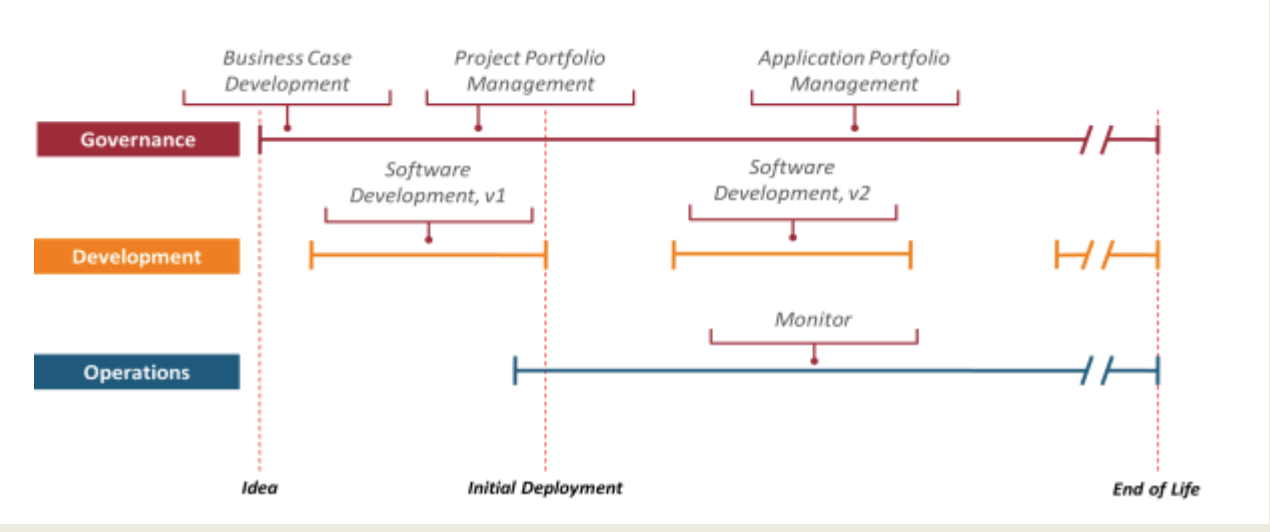
\includegraphics[width=1\textwidth]{Diplomka/Figures/alm.png}
    \caption{Aspekty ALM a jejich fáze \cite{alm_chappell}}
    \label{fig:alm}
\end{figure}

Proces, který probíhá během celého aplikačního cyklu, je řízení. Vzniká počáteční myšlenkou zákazníka a pokračuje až do konce života softwaru. Během této činnosti jsou prováděny rozhodovací procesy, plánování, sběr požadavků a samotné řízení projektu. Je to nejdůležitější aspekt celého aplikačního cyklu. Pakliže by tento proces nebyl správně dodržován, nemusí být naplněna obchodní hodnota daného softwaru. \cite{alm_chappell} První fází, kterou proces začíná, je \textit{Business Case Development}, ve kterém je řešen sběr požadavků zákazníka a vytvoření základní koncepce vývoje. Poté se v~rámci fáze \textit{Project Portfolio Managmentu} řeší procesy spojené s~organizací vývoje a nasazení do produkčního prostředí. V~rámci poslední fáze, která probíhá po nasazení do produkčního prostředí, má manažer na starosti kontrolovat, zda daný software splňuje definované požadavky zákazníka.

Proces vývoje začíná, jakmile je sběr požadavků dokončen a veškeré funkcionality jsou specifikovány. Hlavní část procesu probíhá až do nasazení softwaru do produkčního prostředí. Po nasazení do produkčního prostředí vývoj probíhá již jen v~menších fázích, v~nichž si zákazník přeje dodělat nové požadavky. Nové požadavky na funkčnost mohou vzniknout například proto, aby daný software obstál v~konkurenčním prostředí. \cite{alm_chappell}. V~rámci jednotlivých fází vývoje tedy probíhá postupně nejprve základní první verze daného softwaru. Po nasazení do produkčního prostředí probíhá jednak údržba systému a také vývoj nových funkcionalit (viz obrázek \ref{fig:alm}).

Samotný provoz softwaru začíná ve chvíli, kdy je vývoj dokončen. Provoz probíhá až do úplného ukončení činnosti softwaru. Během tohoto procesu probíhají práce spojené s~během a udržováním aplikace, software je nasazován do produkčního prostředí a je monitorován jeho běh.  \cite{alm_chappell}

Každá část životního aplikačního cyklu se liší dle použitého vývojového procesu. Rozdílně vývoj probíhá při agilním procesu nebo při vodopádovém modelu. Jednotlivým vývojovým procesům se věnuji v~rámci kapitoly \ref{sec:sw_process}.


% ALM aplikace se používají pro plánování a monitorování procesu. Na základě zmonitorovaných dat je poté proces upravován a měněn tak, aby bylo možno produkt dokončit úspěšně při co nejmenších nákladech. Aplikací .

\section{codeBeamer ALM}
\label{sec:codebeamer}
Aplikace codeBeamer obsahuje několik nástrojů používaných pro kompletní správu celého životního cyklu systému, který začíná vývojem systému a pokračuje až do vydání jeho funkční verze. Prakticky životní cyklus systému nekončí vydáním první funkční verze, ale systém je dále udržován a zlepšován dokud je konkurenceschopný nebo využitelný v~daném prostředí. V~rámci aplikace codeBeamer tedy existuje mnoho nástrojů, jež dokáží zajistit správu celého životního cyklu, například správa požadavků, správa testů, správa kvality, správa zacházení s~riziky a mnoho dalších nástrojů. Aplikace je vhodná pro všechny varianty agilního přístupu vývoje. Aplikace také podporuje verzování vyvíjeného systému a následnou práci s~jednotlivými verzemi. \cite{ref:about_codebeamer}

CodeBeamer je koncipován jako jedna velká aplikace obsahující všechny nástroje pro správu životního cyklu aplikace na jednom místě. Velká výhoda tohoto přístupu spočívá v~tom, že máme na jednom místě veškeré informace od úplného začátku životního cyklu až do konce životního cyklu aplikace. Můžeme tedy i zpětně trasovat jednotlivé fáze celého vývoje. CodeBeamer poskytuje několik předdefinovaných šablon pro různé typy vývoje. Mezi ty patří například šablona pro vývoj v~leteckém průmyslu, v~automobilovém průmyslu (šablona pro standard ASPICE) nebo například pro zdravotnictví. Obsahuje také šablony pro různé ostatní procesy, například pro testování, pro zákaznickou podporu nebo SCRUM.  \cite{ref:codebeamer_templates} Šablony jsou užitečné jednak pro začínající tým, který s~vývojem teprve začíná, ale jsou také vhodné pro zajištění dodržování daných procesů, standardů a také pro snížení celkových nákladů na samotný vývoj.

Další výhodou nástroje codeBeamer je, že nabízí velké množství přídavných aplikací či propojení s~jinými, nejen vývojovými nástroji. To je vhodné například pro propojení s~nástroji zákazníka nebo s~ostatními nástroji poskytujícími služby, které codeBeamer neobsahuje. Mezi platformy a nástroje, které lze propojit, patří například Jira, Git, JUnit, Docker, IBM Rational DOORS, Slack a mnoho dalších nástrojů používaných v~rámci celého životního cyklu vyvíjeného systému či aplikace.

CodeBeamer je placený nástroj nabízející výběr z~několika stupňů typů licencí.  Nástroj je možno používat buď jako aplikaci nainstalovanou na vlastním serveru, nebo s~cloudovou licencí přímo na serverech společnosti Intland, která codeBeamer vyvíjí. Nástroj nabízí pro vyzkoušení třicetidenní testovací licenci zdarma. CloudBeamer je možno používat buď jako webovou aplikaci přímo v~prohlížeči nebo jako desktopovou aplikaci na operačním systému Windows a Linux. \cite{ref:codebeamer_pricing}

\subsection{Sběr a správa požadavků}
Aplikace codeBeamer ALM poskytuje v~plné licenci mnoho možností pro sběr a následnou správu požadavků všech různých typů. Správa požadavků obsahuje také správu návaznosti a propojení různých typů artefaktů napříč celým životním cyklem daného projektu či systému s~jinými artefakty a požadavky. Veškerým požadavkům lze přiřadit buď již předpřipravené atributy nebo vytvořit nové vlastní atributy.

Pro navigaci v~rámci celé aplikace a projektu slouží vrchní horizontální menu, které obsahuje položky pro dokumentaci, verzování a administraci a správa požadavků, která se nachází pod položkou \textit{Trackers}. Po rozkliknutí této položky se zobrazí úvodní nástěnka s~konfigurovatelnými bloky, na nichž se mohou umístit různé grafy. Jednotlivým grafům můžeme nastavovat data, ze kterých mají čerpat. Tedy například počet softwarových požadavků v~různých stavech, počet všech požadavků na dané vydání a mnoho dalšího. Celá nástěnka je zobrazena na obrázku \ref{fig:codebeamer_trackers}.

\begin{figure}[!ht]
    \centering
    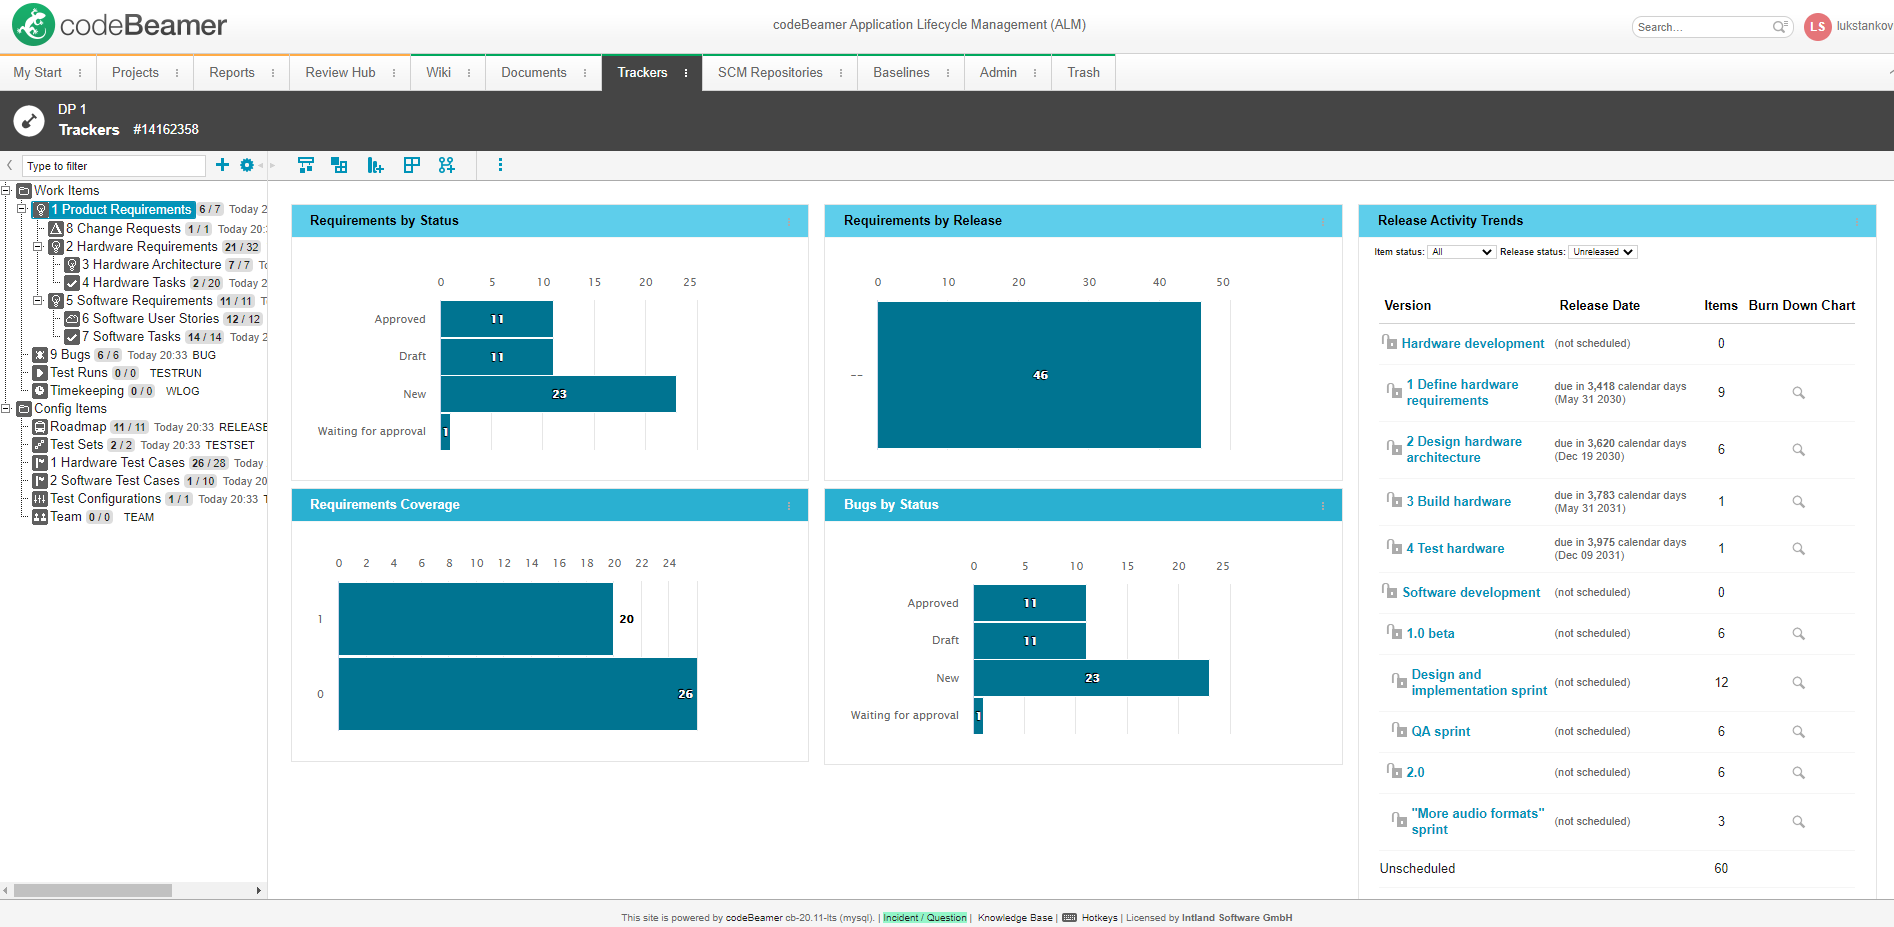
\includegraphics[width=1\textwidth]{Diplomka/Figures/codebeamer_trackers.png}
    \caption{Nástěnka požadavků aplikace codeBeamer ALM}
    \label{fig:codebeamer_trackers}
\end{figure}

Na levé straně obrazovky se nachází navigace obsahující kategorie jednotlivých artefaktů. Po otevření jedné z~kategorií se nám zobrazí seznam artefaktů. Ve výchozím zobrazení se artefakty zobrazí společně se stavy artefaktu a zodpovědné osoby, jako je možno vidět na obrázku \ref{fig:codebeamer_requirments}. Dle potřeby lze sloupce přidávat a upravovat.

\begin{figure}[!ht]
    \centering
    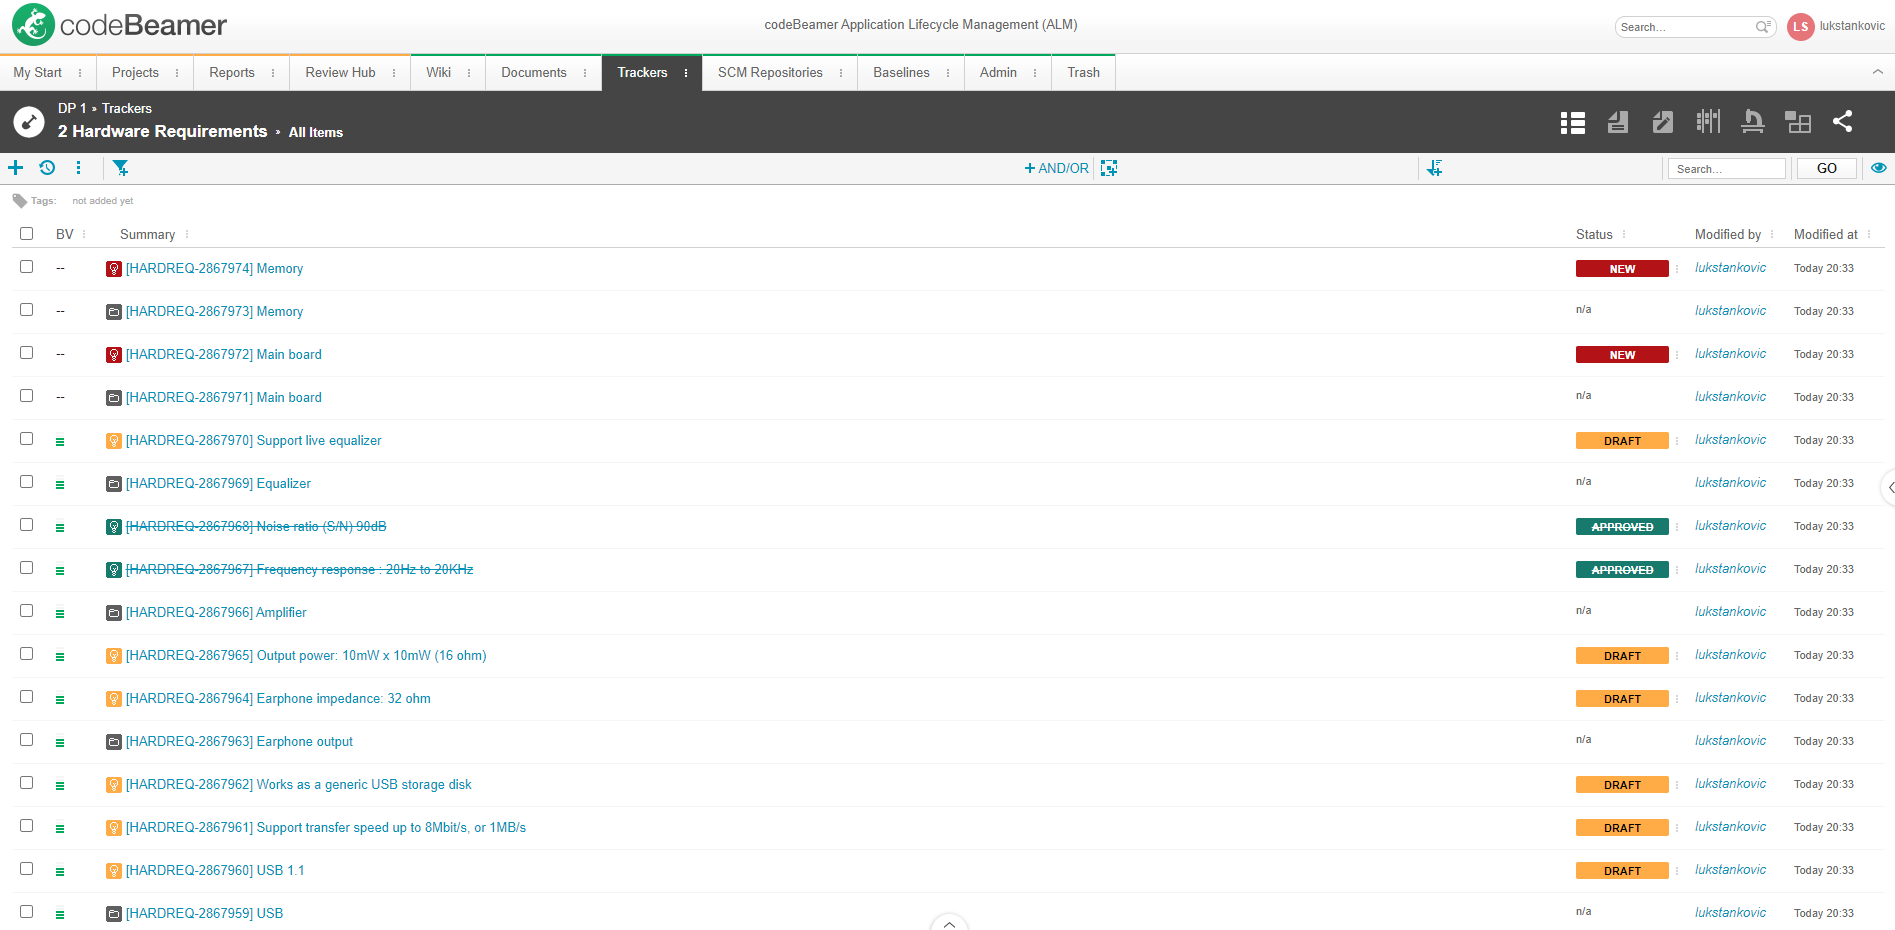
\includegraphics[width=1\textwidth]{Diplomka/Figures/codebeamer_requirments.png}
    \caption{Seznam požadavků v~aplikaci codeBeamer ALM}
    \label{fig:codebeamer_requirments}
\end{figure}

Místo seznamu lze také zobrazit artefakty ve formátu jako dokument, kdy jsou viditelné názvy artefaktů, popis a komentáře. Takové formátování je vhodné pro přehledný výpis a editaci popisů, zadání a komentování artefaktů. Třetí dostupné zobrazení je zobrazení \textit{kanban} tabule, kde jsou artefakty zobrazeny jako lístečky ve sloupcích, jež jsou ve výchozím nastavení \textit{ToDo}, \textit{In progress}, \textit{To verify} a \textit{Done}. Artefakty ve formě lístečků můžeme libovolně přesouvat mezi sloupečky dle definovaného procesu v~rámci projektu. Poslední možné zobrazení \textit{Test coverage} poskytuje vyobrazení, kolik procent artefaktů v~jednotlivých fázích vývoje je pokryto testy, kolik z~nich je vyhovujících a kolik testy neprochází.

U~artefaktů můžeme nastavovat velké množství jak přednastavených atributů, tak si můžeme definovat i atributy vlastní. Toto nastavení je možno provádět v~detailním zobrazení daného artefaktu, nebo v~pravém sloupci po kliknutí na artefakt na výpise všech artefaktů. Na detailu artefaktu můžeme také přidávat komentáře, přílohy anebo spojovat artefakt s~jinými artefakty. Každý artefakt má svůj vlastní identifikátor, pomocí něhož ho můžeme sdílet mezi ostatní kolegy v~rámci vývoje.

\subsection{Monitorování}
Procesy můžeme v~rámci nástroje codeBeamer ALM monitorovat například pomocí metrik. Ty jsou v~grafické podobě bohužel dostupné pouze na nástěnce. Na všech ostatních místech nástroje je zobrazení agregovaných dat pouze textové. Mezi textové metriky můžeme zařadit například pokrytí požadavků testy. Další velkou nevýhodou nástroje codeBeamer je, že neexistuje zobrazení metriky v~určitém časovém období. Pokud si uživatel nebude pravidelně exportovat a manuálně porovnávat jednotlivé metriky, nemůže nijak vyhodnotit postupný vývoj systému.

Z~naměřených dat v~rámci procesu je možno vytvářet tzv. \textit{reporty}. Ty lze vytvářet pomocí speciálního vlastního dotazovacího jazyka podobného SQL. Pomocí napsaných dotazů můžeme naměřená data filtrovat a agregovat dle potřeby a poté exportovat. Tento dotaz lze uložit a následně ho pouze spouštět a tím filtrovaná data zobrazit. Tato data je možno použít pro vygenerování metriky. Nevýhodou tohoto přístupu však je, že je potřeba dotaz vždy ručně načíst a spustit.

\subsection{Export dat}
Jak již bylo zmíněno v~předešlé kapitole \ref{sec:codebeamer}, artefakty a celý systém je možno propojit s~mnoha jinými vývojovými nástroji. Nejkomplexnějším řešením je exportovat data pravidelně pomocí REST API. Ve výchozím stavu je napojení pro všechny uživatele vypnuto a je nutno jej povolit v~nastavení účtu. Velkou výhodou napojení pomocí REST API je, že můžeme data o~jednotlivých artefaktech stahovat pravidelně dle naší potřeby. Veškerá data, která API vrátí, jsou ve formátu JSON. API poskytuje velké množství metod pro různá data. Tyto jednotlivé metody jsou velmi dobře zdokumentovány a popsány v~dokumentaci codeBeameru, která je volně dostupná na internetu.  \cite{ref:codebeamer_rest}

Kromě komplexních exportů pomocí REST API do jiných vývojových nástrojů můžeme také jednotlivé artefakty exportovat do formátu pro Microsoft Office Word a Excel, do formátu CSV nebo do prostého PDF. Takto lze artefakty exportovat manuálně buď jeden artefakt za druhým, nebo najednou všechny artefakty v~dané kategorii. Nevýhodou těchto exportů je, že mohou být provedeny pouze manuálně v~projektu a nelze je automatizovat. Takto exportované artefakty mohou sloužit pouze pro budoucí textovou zálohu artefaktů, jelikož v~datech nelze jednoduše vyhledávat a pracovat s~nimi tak detailně, jako při exportu pomocí REST API.


\section{Siemens Polarion ALM}
Aplikace Polarion slouží jako jednotné řešení umožňující propojit všechny možné účastníky všech procesů v~dané společnosti. Pomocí vestavěných nástrojů dokáže propojit různé týmy vyvíjející určitý systém. Je vhodná pro vývoj velkých systémů nebo aplikací. Mezi takové systémy můžeme zařadit i vývoj nějakého systému v~automobilovém průmyslu. Aplikace stejně jako codeBeamer ALM obsahuje veškeré nástroje pro správu celého životního cyklu vyvíjeného produktu, mezi které patří například správa požadavků, správa kvality systému, správa zacházení s~riziky, správa testů a pokrytí testy a mnoho dalších. Dále aplikace Polarion nabízí automatizaci jednotlivých procesů. \cite{ref:polarion_about}

Siemens Polarion je navržen jako jedna aplikace obsahující mnoho nástrojů pro správu životního cyklu. Tyto nástroje jsou v~navigaci prakticky na jednom místě. Vývojový tým tedy nemusí mít stejně jako v~případě codeBeameru více aplikací a nástrojů pro správu projektu. Aplikace je placená a je možno ji provozovat buď jako webovou aplikaci v~prohlížeči, nebo jako klasickou aplikaci přímo v~systémech Windows a Linux. Stejně jako v~případě aplikace codeBeamer obsahuje Polarion kromě čisté šablony několik šablon, v~nichž je možno pracovat na dalších vyvíjených projektech. Proces vytváření nového projektu z~šablony nebo případně založení čistého a prázdného projektu je možno vidět na obrázku \ref{fig:polarion_new_project}. Vytvořené šablony jsou z~různých prostředí vývoje, například obecný agilní projekt, zdravotnictví nebo dokonce i Automotive SPICE.


\begin{figure}[!ht]
    \centering
    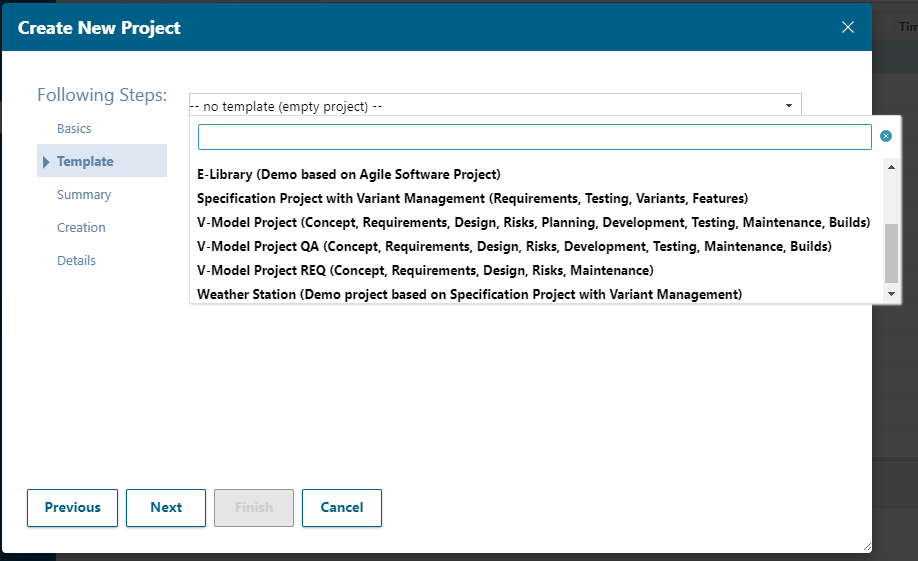
\includegraphics[width=0.8\textwidth]{Diplomka/Figures/polarion_create_project.png}
    \caption{Vytváření projektu v~aplikaci Siemens Polarion ALM}
    \label{fig:polarion_new_project}
\end{figure}


Aplikace v~základu obsahuje nástěnku se základními grafy, stránku s~požadavky, návrhem, riziky, plánováním, vývojem, testováním a údržbou. Další položky jsou v~navigaci ve výchozím stavu skryty a je nutno je povolit. Mezi další položky například patří sestavy, verzování, vydávání nových verzí vyvíjeného systému a mnoho dalších.

\subsection{Sběr a správa požadavků}
Polarion nabízí v~rámci licence veškeré potřebné nástroje pro sběr a správu artefaktů prakticky všech typů. Samozřejmostí je propojení artefaktů s~jinými a tím vytvoření návazností v~rámci celého životního cyklu vytvářeného nebo spravovaného projektu. Artefakty lze řadit do složek a oddílů dle potřeby a logiky. Artefakty je možné přizpůsobovat a přidávat jim vlastní atributy a vlastnosti.

Aplikace obsahuje vertikální navigaci, pomocí níž je možno přecházet do jednotlivých sekcí jako jsou nástěnka, plánování, vývoj a mnoho dalšího. Pro zobrazení požadavků existuje položka \textit{Requirements} obsahující veškeré definované skupiny požadavků v~daném projektu. Na úvodní obrazovce této sekce se nachází přehledný výpis všech kategorií požadavků. Po otevření jedné z~kategorií jsou vypsány veškeré požadavky dané kategorie. Aplikace nabízí několik zobrazení. Výchozím zobrazením je zobrazení jako dokument, kdy jednotlivé požadavky jsou sepsány pod sebou s~popisem jako v~knize. Výhodou tohoto zobrazení je přehlednost. Dalším zobrazením je zobrazení ve stromové struktuře, kdy jsou jednotlivé požadavky odsazeny dle jejich podkategorie a nadpisu. Toto zobrazení je možno vidět na obrázku \ref{fig:polarion_requirements}. Je také možnost zobrazit si veškeré požadavky nestrukturovaně v~tabulce. Dále si lze požadavky různými způsoby zobrazit graficky. Takto je možno zobrazit požadavky na časové ose celého vývoje, v~živém plánu vývoje nebo v~tabulce návazností všech požadavků.

\begin{figure}[!ht]
    \centering
    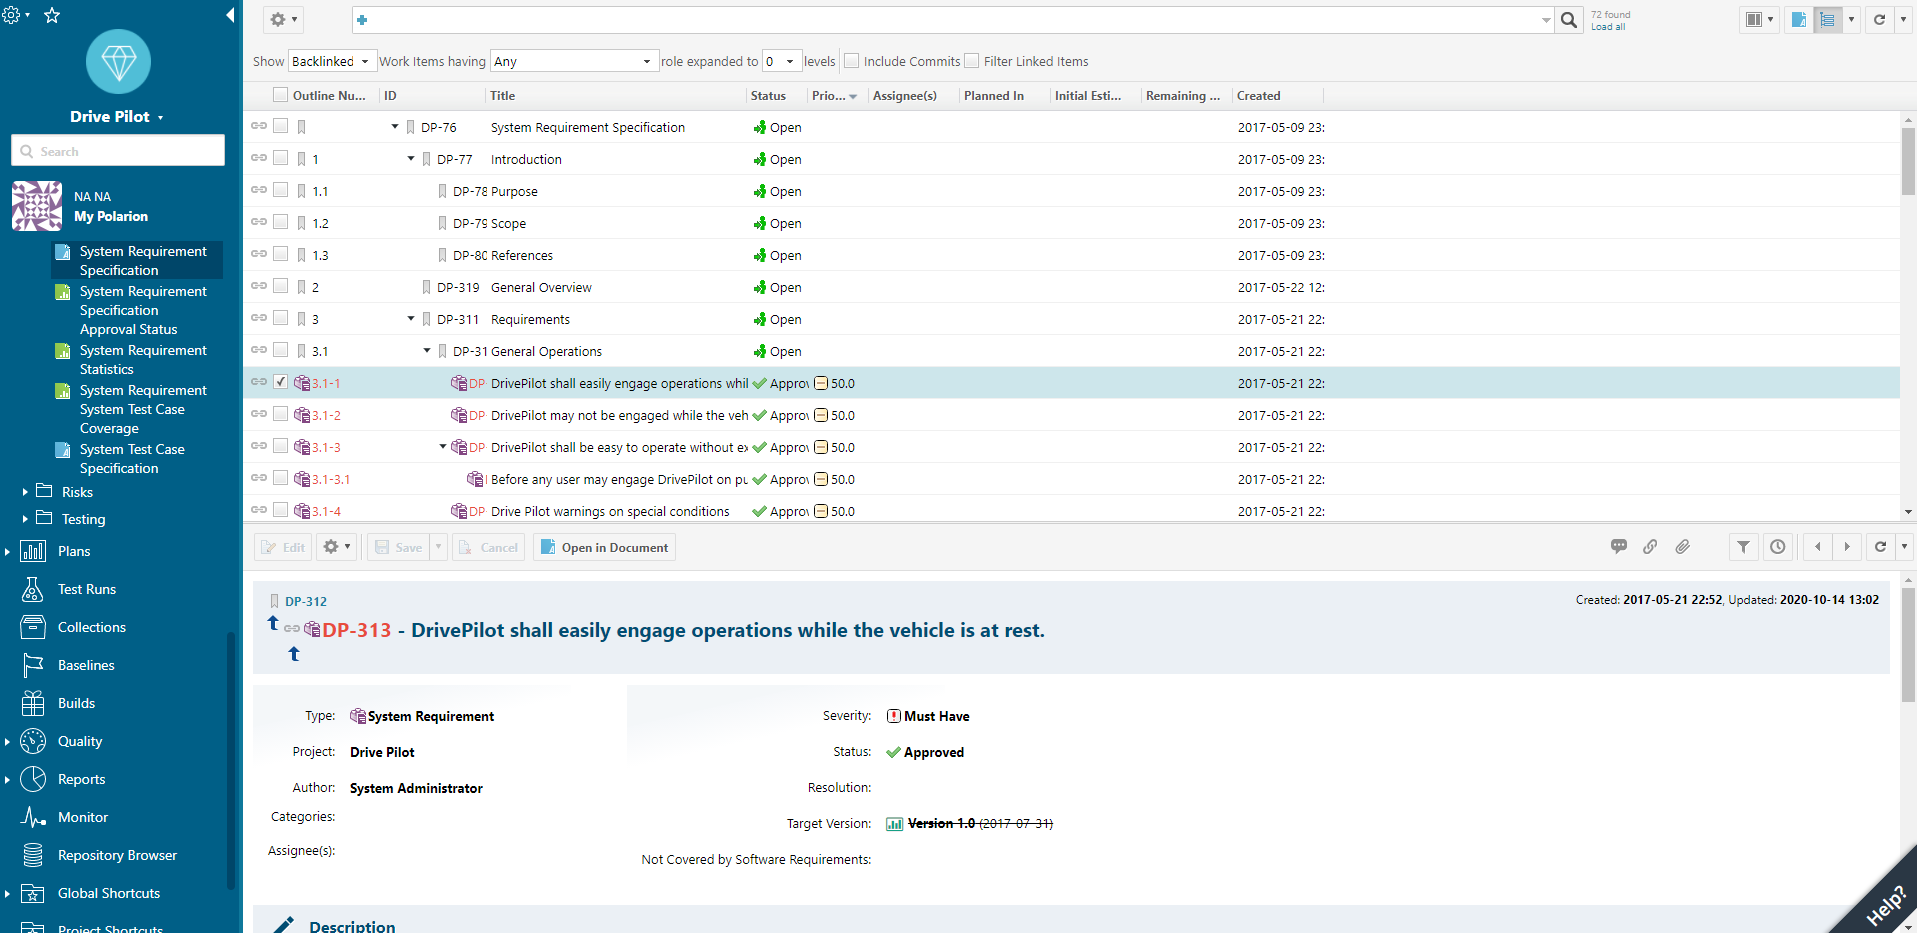
\includegraphics[width=1\textwidth]{Diplomka/Figures/polarion_requirements.png}
    \caption{Seznam požadavků ve stromovém zobrazení v~aplikaci Siemens Polarion ALM}
    \label{fig:polarion_requirements}
\end{figure}

Výhodou oproti aplikaci codeBeamer je, že abychom si zobrazili detail samotného požadavku, nemusíme otevírat celou novou stránku, ale požadavek je nám zobrazen v~menším okně v~dolní části obrazovky. Pokud chceme otevřít požadavek na nové stránce, je třeba jej otevřít pomocí dvojkliku. V~detailu každého požadavku můžeme nastavovat námi definované atributy. Samozřejmostí je unikátní číslo každého požadavku. To navíc obsahuje předponu, kterou si můžeme definovat v~rámci projektu. Jednotlivé požadavky je možno schvalovat, propojovat a přepínat do různých stavů.

\subsection{Monitorování}
Aplikace Polarion nabízí monitorování procesů pomocí metrik, které je možno zobrazit na vícero místech. Prvním místem, kde lze metriku zobrazit, je nástěnka. Zde se ve výchozím stavu v~šabloně pro agilní projekt zobrazuje graf, kolik úkolů je třeba ještě do dalšího vydání dokončit, kolik chyb bylo nalezeno a mnoho dalšího. Veškeré metriky na nástěnce jsou zobrazeny graficky. Grafy není možno bohužel nijak filtrovat, jde pouze o~rychlé informace poskytující lepší orientaci o~stavu, v~němž se projekt nachází. Nástěnku je možno vidět na obrázku \ref{fig:polarion_dashboard}.

\begin{figure}[!ht]
    \centering
    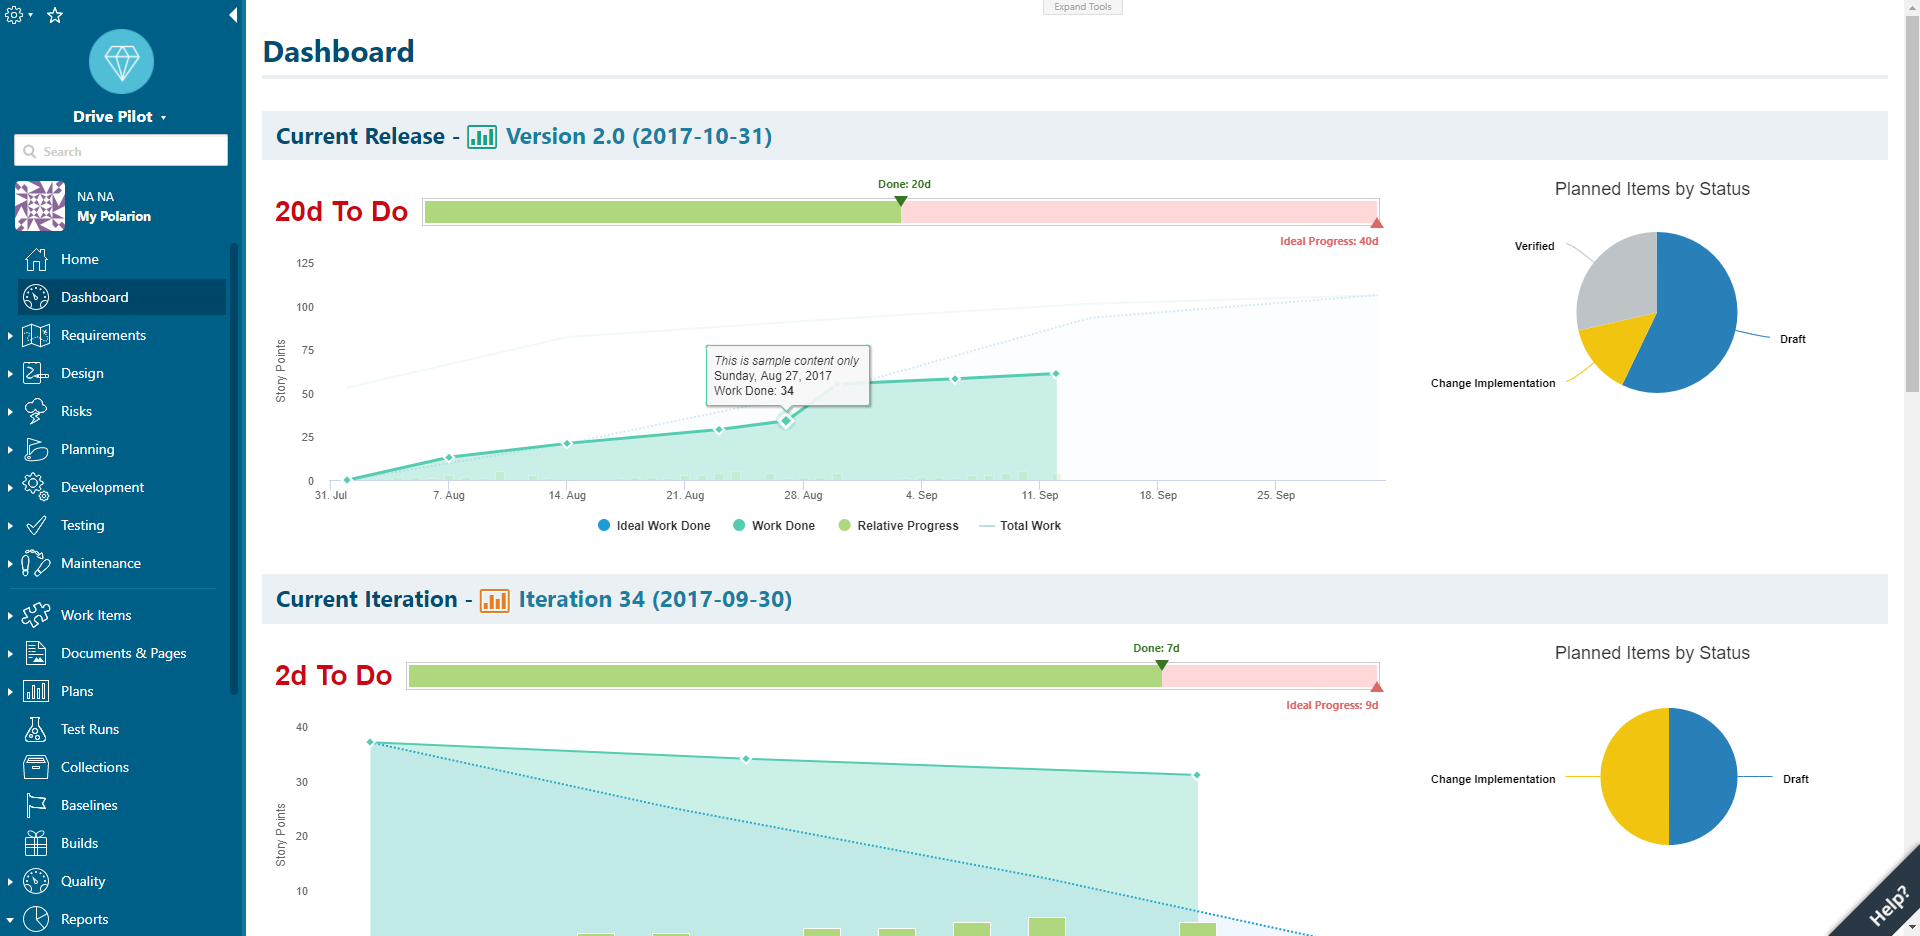
\includegraphics[width=1\textwidth]{Diplomka/Figures/polarion_dashboard.png}
    \caption{Nástěnka a metriky v~aplikaci Siemens Polarion ALM}
    \label{fig:polarion_dashboard}
\end{figure}

Dalším místem, kde je možno metriky zobrazit,  je záložka \textit{Plans}. Zde je možno zobrazit metriky jak v~grafickém tak tabulkovém zobrazení. Uživatel si může metriku definovat a vytvořit pomocí filtrů v~horní části obrazovky. Do jednotlivých metrik si uživatel může navolit různé typy artefaktů. Metriky zde není bohužel možno nijak rychle filtrovat a upravovat. Celý výpis metrik je možno si exportovat do formátu PDF. Bohužel nelze exportovat jen určité grafy a výpisy, ale pouze celou stránku s~metrikami.

Grafické zobrazení průběhu vývoje projektu je možno zobrazit napříč celou aplikací Siemens Polarion. Je možno například zobrazit si graficky vývoj testování vyvíjeného systému, nové verze k~vydání, vytvářet různé reporty s~definovanými pravidly a mnoho dalšího. Velkou nevýhodou však je, že na žádném místě není možno nijak podrobněji filtrovat a upravovat grafy.

\subsection{Export dat}
K~aplikaci Siemens Polarion je možno pomocí doplňků připojit velké množství jiných vývojových nástrojů. Existuje například doplněk pro propojení s~aplikací Jira. Většina těchto doplňků je placených. \cite{ref:polarion_extensions}

Další možností exportu dat je manuální export jednotlivých artefaktů do formátu PDF. Takto provedený export nelze použít pro agregování dat, ale pouze pro prostou dokumentaci či zálohu. Druhou nevýhodou je nemožnost proces jakkoli zautomatizovat, je potřeba PDF exportovat manuálně v~aplikaci. Do PDF je možno exportovat prakticky každý artefakt, výpis dat nebo celou stránku s~metrikami.

Siemens Polarion nabízí export dat pomocí webových služeb. Ty jsou podrobně zdokumentovány na veřejně přístupné dokumentaci. \cite{ref:polarion_documentation} Výhodou tohoto přístupu je, že můžeme proces exportu dat automatizovat a data si z~aplikace stahovat kdykoli potřebujeme. Takto můžeme z~Polarionu vyexportovat velké množství informací. Nevýhodou této metody je, že export může být složitější než použití například REST API.

Poslední, a dle autorů aplikace nejkomplexnější, možností exportu dat je čtení dat přímo z~databáze Polarionu. Pomocí exportu dat z~databáze můžeme také tento proces automatizovat a spouštět dotazy nad databází prakticky kdykoli. Dokumentace obsahuje kompletní architekturu databáze včetně ukázkových SQL dotazů. \cite{ref:polarion_documentation} V~dokumentaci se kromě propojení jednotlivých tabulek nachází také popis všech objektů v~databázi. Velkou výhodou této metody je možnost exportovat jakékoliv data, k~nimž máme v~databázi přístup. Nevýhodou je, že pro vytvoření exportu potřebujeme znát architekturu databáze, abychom mohli napsat SQL dotaz, který nám data zobrazí. Jelikož je databáze velmi komplexní, může studování architektury a psaní SQL dotazů výrazně navýšit náročnost vytváření exportů.

\section{IBM Jazz}
Je to velmi robustní a komplexní platforma poskytující podporu a zázemí během celého životního cyklu systému. Stejně jako ostatní aplikace používané pro správu životního cyklu vyvíjeného systému je hlavním cílem to, aby správa i vývoj byly co nejefektivnější, aby byl životní cyklus monitorován a aby si jednotlivé vývojové týmy jednodušeji vyměňovaly potřebné informace. Celá platforma Jazz poskytuje veškeré potřebné nástroje pro organizaci celého životního cyklu produkovaného systému. Jazz dokáže například spravovat a trasovat požadavky, vizualizovat data, obsahuje metriky a mnoho dalšího. \cite{ref:jazz}

IBM Jazz není jedna aplikace jako v~případě aplikace codeBeamer nebo Siemens Polarion, ale velká platforma složená z~několika nezávislých aplikací. Tyto aplikace nejsou nijak propojeny a jsou tedy plně nezávislé. Tato vlastnost může být brána pro některé společnosti jako nevýhoda, jelikož musí spravovat více instancí aplikací a ne pouze jednu, která obsahuje veškeré funkcionality. Jednotlivé aplikace jsou primárně koncipovány jako webové aplikace. Není tedy potřeba řešit instalaci aplikací na počítač nebo kompatibilita s~různými operačními systémy. Pokud by to prostředí dané společnosti vyžadovalo, existují aplikace a rozšíření založené na nástrojích Visual Studio a Eclipse.

IBM Jazz je komerční a tedy placená platforma, která může být provozována v~cloudu společnosti IBM nebo na vlastním serveru. Velkou nevýhodou je, že při instalaci je potřeba následovat složité manuály, jelikož platforma nedisponuje žádnou jednoduchou instalaci, například pomocí virtualizace Docker. V~rámci platformy IBM Jazz existují při vytváření základní šablony, z~nichž můžeme projekt vytvořit.  Na výběr jsou například šablony pro agilní vývoj pomocí metody Scrum, pro klasický tradiční vývoj bez iterací a mnoho dalších.


\subsection{Nástroje a aplikace IBM Jazz}
Jak již bylo zmíněno, IBM Jazz je pouze platforma nabízející různé nástroje a aplikace, které nejsou na sobě závislé a jsou plně oddělené. Jelikož je nástrojů mnoho a jsou zaměřené na různá odvětví, budu se věnovat aplikacím a nástrojům určeným pro správu životního cyklu vyvíjené aplikace. \cite{ref:jazz_products}

\begin{itemize}
\item \textit{IBM Engineering Requirements DOORS Next} -- v~rámci této aplikace dokážeme vytvářet, spravovat a analyzovat jednotlivé požadavky. V~aplikaci dokážeme také evidovat propojení jednotlivých požadavků a zobrazovat metriky ohledně požadavků.
\item \textit{IBM Engineering Workflow Management} -- aplikace obsahuje správu spolupráce mezi jednotlivými odděleními dané společnosti při vývoji. Můžeme zde zařadit například plánování, iterace procesů, verzování vyvíjeného systému, automatizace vydávání a další.
\item \textit{IBM Engineering Test Management} -- slouží zejména pro plánování a organizaci testování vyvíjeného systému. Aplikace podporuje sdílení dat mezi ostatní pracovníky.
\item \textit{IBM Engineering Systems Design Rhapsody - Model Manager a Design Management} -- pomocí této aplikace je možno navrhovat a spravovat návrh architektury a designu celého systému.
\item \textit{IBM Engineering Lifecycle Optimization - Publishing} -- v~rámci aplikace dokážeme generovat a vytvářet dokumenty napříč všemi nástroji platformy Jazz. Výsledné dokumenty je možno exportovat do různých formátů, mezi něž patří PDF, HTML, Microsoft Office a další.
\item \textit{Jazz Reporting Service} -- aplikace je alternativou k~vytváření sestav a metrik, které jsou k~dispozici v~jiných aplikacích v~rámci IBM Jazz. Aplikace je propojená s~ostatními Jazz aplikacemi a podporuje agregaci dat ze všech různých aplikací. V~rámci aplikace je možno agregovaná data exportovat do různých formátů. Pro samotné vytváření a agregování existuje v~aplikaci nástroj \textit{Report Builder}.
\end{itemize}

Veškeré tyto aplikace je možno mít pod jednou licencí v~rámci nástroje \textit{IBM Engineering Lifecycle Management} a to buď nainstalované na vlastním serveru, nebo v~cloudu u~společnosti IBM. Veškeré dostupné aplikace můžeme nalézt na webových stránkách společnosti IBM. \cite{ref:jazz_products}

\subsection{Sběr a správa požadavků}
Správu požadavků v~rámci platformy IBM Jazz je možno provádět v~aplikaci \textit{IBM Engineering Requirements DOORS Next}. Ta obsahuje veškeré potřebné nástroje pro sběr a správu požadavků všech možných typů. Veškeré požadavky lze jakkoli propojovat s~ostatními požadavky v~rámci vyvíjeného projektu. V~aplikaci je možno vytvářet vlastní typy požadavků, které lze řadit do vlastních složek a oddílů dle potřeby a logiky daného projektu. Požadavkům je možno přidávat jakékoli předdefinované či vlastní atributy a vlastnosti.

Stejně jako předešlé aplikace obsahuje vertikální navigaci, pomocí níž je možno přecházet mezi jednotlivými typy požadavků. Po otevření jednoho z~typů požadavků jsou vypsány veškeré požadavky daného typu. Aplikace nabízí několik druhů a možností zobrazení tohoto výpisu. Typy výpisů jsou prakticky identické jako v~aplikaci codeBeamer a Polarion. Existuje zde například výpis typu dokument, kdy jsou požadavky vypsány jako v~dokumentu v~aplikaci Microsoft Word pomocí nadpisů a popisů. Takový výpis je možno vidět na obrázku \ref{fig:ibm_doors_req}. Dále zde existuje základní výpis jednotlivých požadavků v~samostatných řádcích anebo ve tvaru stromu, kdy jsou požadavky odsazeny dle adresáře, do něhož patří.

\begin{figure}[!ht]
    \centering
    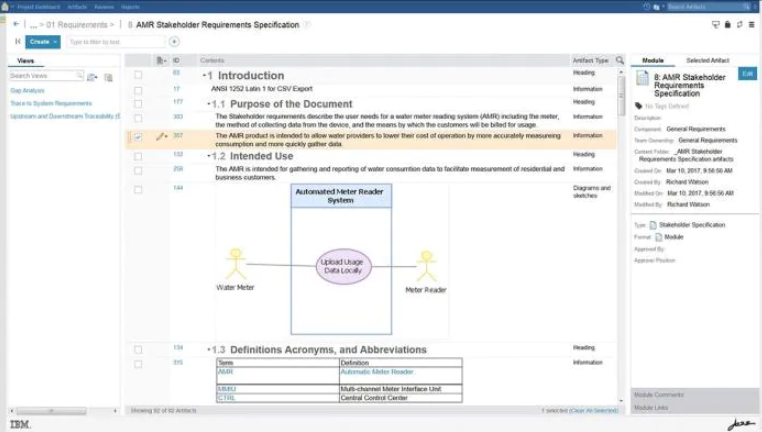
\includegraphics[width=1\textwidth]{Diplomka/Figures/ibm_doors_ng_req.png}
    \caption{Výpis požadavků v~zobrazení dokumentu v~aplikaci IBM Engineering Requirements DOORS Next (převzato z~\cite{ref:ibm_jazz_erm_dn})}
    \label{fig:ibm_doors_req}
\end{figure}
Atributy a vlastnosti k~danému atributu je možno nastavit buď přímo ve výpisu požadavků, anebo v~detailním okně daného požadavku. V~administraci aplikace je možno vytvářet nespočet typů atributů, které můžeme poté požadavkům přiřazovat a filtrovat podle nich. Samozřejmostí je možnost požadavkům nastavovat různé předdefinované nebo vlastní stavy a propojovat je s~ostatními požadavky. U~jednotlivých požadavků si můžeme zobrazit nejen veškeré přílohy a komentáře, ale také historii úprav daného požadavku. Historie úprav je bohužel pouze pro zobrazení, kdy byl daný požadavek upravován, a ne co přesně bylo v~danou dobu měněno. Každý požadavek má vlastní identifikátor, kterým je možno jej identifikovat napříč celou aplikací.

\subsection{Monitorování}
V~rámci platformy IBM Jazz lze provádět monitorování všech procesů v~aplikaci \textit{Jazz Reporting Service}. Tato aplikace nám zajistí za pomoci nástroje \textit{Report builder} vytváření agregovaných a filtrovaných dat. Výhodou je, že data mohou pocházet z~jakékoli aplikace platformy IBM Jazz. Nejčastěji data pochází z~aplikace pro správu požadavků. Pomocí takto agregovaných dat si můžeme vytvářet a generovat metriky. Vytváření sestavy je možno vidět na obrázku \ref{fig:ibm_reporting_service}. Tato data lze exportovat například do aplikace Microsoft Office. Definovanou metriku je možno zobrazit buď jako graf, nebo jako pouhou tabulku. Toto řešení má bohužel velkou nevýhodu spočívající ve formě chybějících historických dat. Jazz Reporting Service zobrazuje v~grafu vždy pouze aktuální data a aktuální stav jednotlivých požadavků (například v~jakém stavu se nacházejí). Neexistuje zde žádný způsob, jak monitorovat průběh procesu a změny jednotlivých požadavků v~čase. Jedinou vhodnou možností řádného monitorování je vytvoření externí aplikace napojené na celou platformu IBM Jazz.

\begin{figure}[!ht]
    \centering
    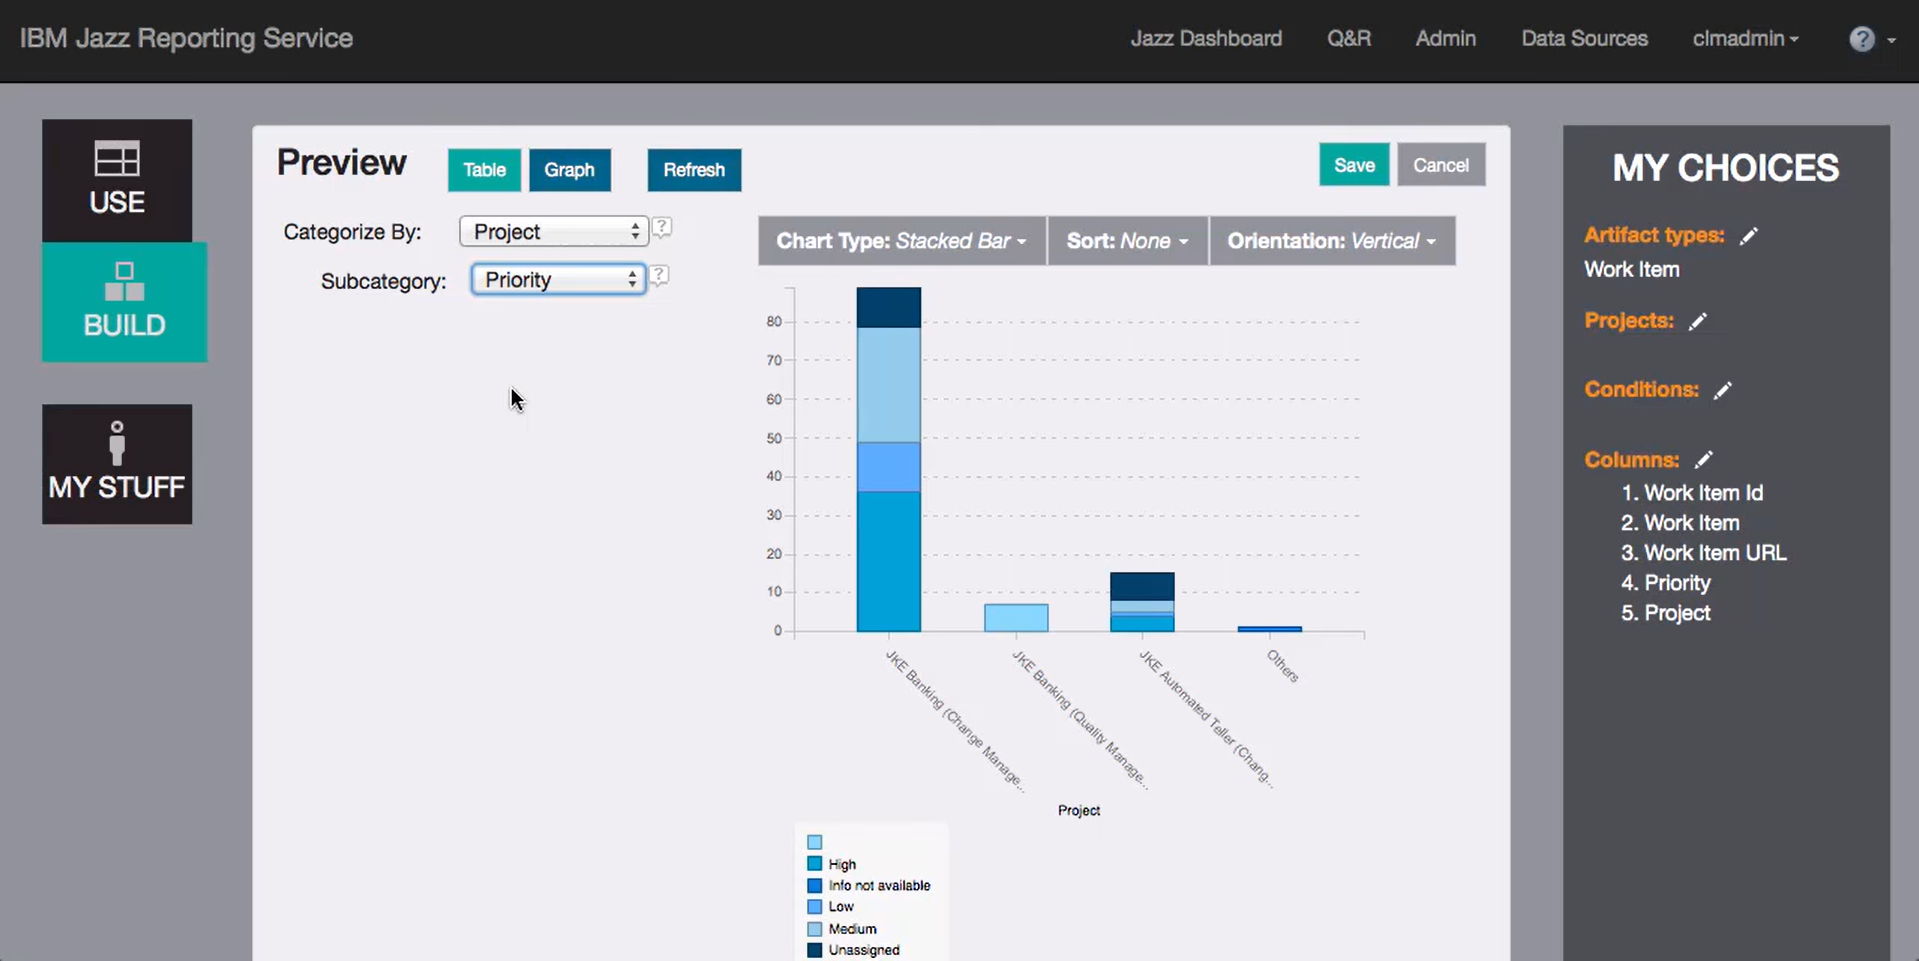
\includegraphics[width=1\textwidth]{Diplomka/Figures/ibm_reporting_service.png}
    \caption{Aplikace Jazz Reporting Service}
    \label{fig:ibm_reporting_service}
\end{figure}

Další možností metrik spojených se sběrem a správou požadavků je zobrazení přímo na nástěnce aplikace \textit{IBM Engineering Requirements DOORS Next}. Vizualizace je takto dostupná pouze omezeně pomocí uživatelských widgetů. Ty jsou pouze náhledové a nelze v~nich efektivně filtrovat. Monitorování v~této aplikaci není nijak pokročilé, má pouze informativní charakter pro rychlé posouzení stavu vývoje.

Abychom mohli monitorovat průběh celého procesu a změny jednotlivých artefaktů, je jedinou možností využít služeb třetích stran či případně si vytvořit vlastní aplikaci pro vytváření a definování metrik. Jednou možností je využít agregování dat pomocí Jazz Reporting Service nebo tato data agregovat ve vlastní aplikaci.

\subsection{Export dat}
V~jednotlivých aplikacích platformy IBM Jazz je možno provést exporty dat dané aplikace. V~základu lze napojit jiné aplikace třetích stran pomocí doplňků s~jinými aplikacemi pro správu vývoje. Takové rozšíření si můžeme naprogramovat i sami dle dokumentace dané aplikace.

Další základní možností exportu dat je možnost exportu jednotlivých požadavků do PDF. Takový export probíhá manuálně a není možno jej použít pro agregaci dat a následnou práci s~nimi a jejich vizualizaci. Takové řešení je vhodné například pro dokumentaci nebo zálohu daných artefaktů a požadavků. Další možností manuálního exportu dat je export všech artefaktů do formátu CSV. Tato data je již možno agregovat a pracovat s~nimi. Nevýhodou však je, že je vždy potřeba pracovníka, který tato data manuálně stáhne.

Platforma IBM Jazz nabízí několik možností přímého napojení a automatického exportování dat. V~rámci této práce se věnuji exportu dat z~aplikace \textit{IBM Engineering Requirements DOORS Next}, kde existují tyto možnosti napojení:

\begin{itemize}
\item DOORS Next Generation Rest API (RRC Reportable API),
\item Reportable REST API,
\item Process REST API (DraftTeamProcessRestApi),
\item Resource Oriented Work Item API with OSLC 1.0 CM,
\item Work Items Service provider for OSLC 2.0 CM,
\item Reportable REST API,
\item napojení na databázi.
\end{itemize}

Jednotlivým možnostem těchto napojení se budu věnovat v~praktické části této práce. Nevýhodou je, že tato API nejsou dobře veřejně dokumentována a je potřeba tedy napojení zkoušet a procházet fóra přímo na stránkách IBM. Další nevýhodou špatné dokumentace je špatná informovanost o~aktuálnosti a funkčnosti daného napojení. Data je možno také exportovat pomocí nástroje OSLC, kterému se budu v~praktické části této práce věnovat.

Poslední možností exportu dat je využití aplikace \textit{Jazz Reporting Service}. Data z~této aplikace si můžeme již předem agregovat a vytvořit metriky, které je možno exportovat například do aplikace Microsoft Excel. Výhodou tohoto přístupu je, že můžeme data filtrovat a agregovat přímo na straně IBM Jazz, která obsahuje již různé předdefinované filtry a není třeba nic složitě programovat. Nevýhodou je však svázání s~touto aplikací a při jakékoli změně v~datech je nutno vytvářet filtry znovu. Další velkou nevýhodou je, že nedokážeme data jednoduše pomocí tohoto přístupu verzovat a udržovat jejich historii přímo na straně IBM. Je tedy potřeba si souběžně vytvořit externí aplikaci na udržování historických dat. Tento přístup při velkém počtu dat ztrácí bez nějaké automatizace smysl i výhody.

\section{Porovnání aplikací}
Všechny tři analyzované aplikace se zaměřují na správu životního cyklu vyvíjeného systému nebo produktu. Analyzované aplikace poskytují nástroje pro sběr a správu požadavků. Samozřejmostí je seznam a výpis všech požadavků, které mohou být zařazeny do jednotlivých kategorií. Požadavkům je možno nastavovat různé popisy, atributy, vlastnosti a spojení s~jinými požadavky nebo artefakty. Ve všech těchto aplikacích je možnost vytvářet vlastní typy a názvy jednotlivých atributů. Lze také vytvářet vlastní názvy a typy propojení mezi artefakty. Všechny analyzované aplikace mají základní stránku s~nástěnkou, na níž se nacházejí základní informace a rychlé metriky o~procesech v~rámci vývoje daného projektu. Všechny tři aplikace také fungují jako webové aplikace nebo desktopové aplikace. Dále jsou aplikace komerční a tedy placené a následně provozované buď na vlastním serveru nebo v~cloudu dané společnosti, která aplikaci poskytuje.

Rozdíl ve správě požadavků mezi aplikací codeBeamer ALM a Siemens Polarion ALM spočívá v~tom, že codeBeamer kombinuje sběr všech artefaktů s~jednotlivými požadavky, zatímco Siemens Polarion má pro veškeré typy artefakty samostatné stránky s~výpisy a metrikami, které jsou uzpůsobeny pro daný typ artefaktu.

Aplikace codeBeamer ALM a Siemens Polarion jsou téměř identické v~tom, že jde o~robustní platformy poskytující veškeré potřebné nástroje pro správu životního cyklu v~rámci jedné aplikace. Oproti tomu platforma IBM Jazz poskytuje tyto nástroje v~jednotlivých aplikacích na různých doménách, které spolu ne vždy správně komunikují.

Největší rozdíl v~aplikacích spočívá v~přístupu ke generování a vytváření metrik. Aplikace codeBeamer obsahuje metriky v~grafické podobě pouze na nástěnce. Tato data jsou pouze informativní. Agregovaná a filtrovaná vlastní data se dají zobrazit pouze textově. Další nevýhodou této aplikace je, že nenabízí žádnou možnost zobrazit si automatické metriky v~určitém časovém období. V~aplikaci lze vytvářet sestavy pomocí jazyka podobného SQL. Sestavy lze vytvářet a spouštět pouze manuálně a nelze je tedy nijak automatizovat. Z~dat získaných vlastním dotazem bohužel nedokážeme vytvořit a definovat vlastní metriku.

Aplikace Siemens Polarion obsahuje základní metriky taktéž na nástěnce a nenabízí žádné filtrování a volbu zobrazení. I~tato data jsou pouze informativní. Metriky poskytují pouze rychlé informace o~tom, zda daný vývoj probíhá v~souladu s~plány. Podrobnější metriky a grafy je možno nalézt na specializované stránce. Uživatel si může definovat a vytvořit metriku pomocí filtrů na dané stránce. Bohužel chybí rovněž definování trendové metriky v~čase. Další nevýhoda spočívá v~tom, že Polarion nenabízí podrobný export výsledků dané metriky, ale pouze export do PDF celé stránky s~více metrikami.

Platforma IBM Jazz nabízí kompletně jiný přístup. Kromě nástěnky stejné jako u~ostatních aplikací, kde se nacházejí rychlé informace o~postupu vývoje, existuje samostatná aplikace \textit{Jazz Reporting Service}. V~té je možno pomocí nástroje \textit{Report Builder} vytvořit a definovat na základě filtrů metriky z~jednotlivých artefaktů jiných aplikací platformy IBM Jazz. Definované metriky je možno si zobrazit jak graficky, tak v~tabulce. Tato agregovaná data lze exportovat například do služby Microsoft Office. Velkou nevýhodou je, že definované metriky nezobrazují vývoj v~čase, ale pouze aktuální hodnoty v~daném čase.

Hlavní výhodou těchto aplikací je zachycení a správa vývoje celého systému. Další výhodou je možnost komunikace a spolupráce s~jednotlivými týmy při vývoji. Všechny analyzované aplikace mají prakticky stejný design a liší se pouze v~drobnostech. Bohužel žádná analyzovaná ani jiné nalezené aplikace nesplňují požadovaný účel a funkcionality, tedy možnost vytvářet a generovat trendové metriky a uchovávat v~metrikách historická data.

\begin{table}[htp]
\begin{tabular}{@{}lccc@{}}
\toprule
\textbf{}                     & \textbf{codeBeamer ALM} & \textbf{Siemens Polarion} & \textbf{IBM Jazz} \\ \midrule
Webová aplikace               & ano                     & ano                       & ano               \\
PC aplikace                   & ano                     & ano                       & ne                \\
Jedna velká robustní aplikace & ano                     & ano                       & ne                \\
Export dat pomocí API         & ano                     & ano                       & ano               \\
Historická data               & ne                     & ano                       & ne                \\
Základní definice metrik      & ano                     & ano                       & ano               \\
Pokročilejší metriky graficky & ne                      & ne                        & ano               \\
Metriky potřebné pro ASPICE  & ne                      & ne                        & ne                \\ \bottomrule
\end{tabular}
\caption{Porovnání jednotlivých aplikací a nástrojů pro ALM}
\label{tab:alm_porovnani}
\end{table}

Všechny tři aplikace obsahují možnost přístupu pomocí webové aplikace, přičemž pouze codeBeamer a Siemens Polarion poskytují přístup pomocí počítačové aplikace. Další rozdíl mezi platformou IBM Jazz a ostatními aplikacemi, které jsou řešeny jako jedna velká robustní aplikace, spočívá v~tom, že IBM Jazz je koncipována jako více menších aplikací. Všechny aplikace obsahují export dat pomocí API, přičemž Siemens Polarion nabízí export i přímo z~databáze poskytující více možností než jen API, které je řešeno pomocí webových služeb. IBM Jazz a codeBeamer podporují export pomocí REST API. Až na aplikaci Polarion neposkytuje IBM Jazz ani codeBeamer historické údaje v~metrikách. Bohužel Siemens Polarion nabízí tyto informace pouze omezeně. Jediná platforma IBM Jazz podporuje pomocí \textit{Jazz Reporting Service} pokročilejší zobrazení metriky pomocí grafů. Ostatní dvě aplikace v~základu podporují zobrazení metrik pomocí grafů limitovaně. Ani jedna z~analyzovaných aplikací však neposkytuje zobrazení a definice metrik pro sběr požadavků, které je nutné sledovat dle standardu Automotive SPICE. Rychlý přehled analyzovaných aplikací a nástrojů je možno nalézt v~tabulce \ref{tab:alm_porovnani}.

\newpage % ODSTRANIT
\chapter{Business intelligence}
Dnešní společnosti pracující na velkých a komplexních systémech skladují a spravují při vývoji velká množství dat. S~těmito daty je nutno, nejen pro potřeby analýzy, pracovat a přistupovat k~nim. K~zajištění správných a tedy úspěšných manažerských rozhodnutí je třeba data pochopit a vyčíst z~nich důležité informace. Pomocí získaných a pochopených informací dokážeme informace přeměnit ve znalosti a použít je k~predikcím. Následně dokážeme odhadnout, kam se může vývoj projektu nebo společnosti ubírat.

Jelikož v~drtivé většině jsou sbíraná a analyzovaná data velká a komplexní, nemusí pouhý pohled do tabulky obsahující data celého podniku odhalit nějaká slabá místa. Také si nemusíme takto velká data obsahující i miliony záznamů dostatečně představit. Z~toho důvodu potřebujeme využít nástroje a přístupy, které nám zajistí jednodušší analýzu, nebo data připraví tak, aby je mohl lidský mozek nejen pochopit, ale uvědomit si i souvislosti.

Mezi nástroje a přístupy, pomocí nichž dokážeme data analyzovat a číst, patří například dolování dat, prediktivní modelování, statistika a mnoho dalších přístupů. Mezi nejznámější a nejdůležitější však patří vizualizace dat pomocí grafů. Pomocí vizualizace můžeme provést buď analýzu, nebo pouhou prezentaci pro zjištění, jakým směrem se vývoj ubírá. Těmito oblastmi se právě obor \textit{Business intelligence} zaobírá.

Konkrétně David Loshin \cite{ref:bi_loshin_david} a Data Warhouse Institute \textit{Business intelligence} definují jako procesy, technologie a nástroje potřebné k~přeměně data na informace, informace na znalosti a dále znalosti na plány, které podporují úspěšná rozhodnutí a ziskové obchodní akce. \textit{Business intelligence} zahrnuje obchodní analytické nástroje, datové sklady a správu obsahů a znalostí. Důležité je, že \textit{Business intelligence} nejsou pouze nástroje a aplikace, ale celé procesy realizované správnými lidmi, kteří dokáží tyto informace proměnit v~plány.

Podle Davida Loshina \cite{ref:bi_loshin_david} správné použití \textit{business intelligence} může vést k~mnoha pozitivním změnám, mezi které například patří:

\begin{itemize}
\item \textit{Zvýšení ziskovosti} -- business intelligence dokáže například vedoucím vyhodnotit a provést rozhodnutí, zefektivnění procesů, personální změny, které mohou vést ke zvýšení zisků celé společnosti.
\item \textit{Snížení nákladů} -- s~předchozím bodem samozřejmě souvisí i snížení nákladů, které vzniknou po optimalizovaní procesů, nákladů na skladování nebo snížení investic na základě rozhodnutí dle business intelligence.
\item \textit{Zlepšení vztahů se zákazníkem} -- tohoto benefitu můžeme dosáhnout pomocí analýzy agregovaných informacích o~zákaznicích a následně vylepšit zákaznické služby.
\item \textit{Snížení rizik} -- pomocí analýzy informací dokážeme lépe předem definovat a nalézt rizika, která mohou během vývoje nebo prodeje produktu nastat,
\item a mnoho dalšího.
\end{itemize}

K~zajištění provedení \textit{business intelligence} nám slouží nástroje a aplikace pro tuto činnost vytvořené. Takové aplikace nám dokážou poskytnout historické, aktuální a případně budoucí zobrazení dat. Dále nám poskytují nástroje pro tvorbu sestav, metrik, grafů, nástěnek, sdílení dat mezi ostatními zaměstnanci a spoustu dalších nástrojů. Mezi nejznámější aplikace patří Qlik Sense a Microsoft Power BI, které jsou podrobně popsány v~kapitolách \ref{sec:qlik} a \ref{sec:microsoft_power_bi}. Tyto aplikace byly také doporučeny vedoucím práce Ing. Svatoplukem Štolfou, PhD.

\section{Qlik Sense}
\label{sec:qlik}
Qlik Sense je rozsáhlý analytický nástroj společnosti Qlik, zajišťující integraci dat ze široké škály datových zdrojů. Pomocí aplikace dokážeme přeměnit surová data z~tabulek a databází do vizuální a srozumitelné podoby. Stejně jako u~ostatních podobných \textit{business intelligence} aplikací Qlik Sense obsahuje nástěnky, tvorbu a zobrazení sestav nebo také propojování datových zdrojů. Aplikace podporuje připojení k~široké škále různých jiných aplikací pomocí API, napojení na velké množství databází a také samozřejmě nahrávání datových souborů napřímo jako například CSV, XML, JSON či velké množství dalších formátů. Mezi společnosti používající Qlik Sense patří například Cisco, BP nebo také Samsung. \cite{ref:qlik_general}

Přístup k~aplikaci pro uživatele je možný jednak pomocí aplikace pro počítač a mobilní zařízení, ale také pomocí webové aplikace, která je dostupná přes prakticky jakýkoli webový prohlížeč. Qlik Sense je placená aplikace, která může být provozována buď na vlastním serveru nebo v~cloudu přímo u~společnosti Qlik. Přitom při provozu na vlastním serveru není cena licence vázána na počet uživatelů používajících aplikaci.

\begin{figure}[!ht]
    \centering
    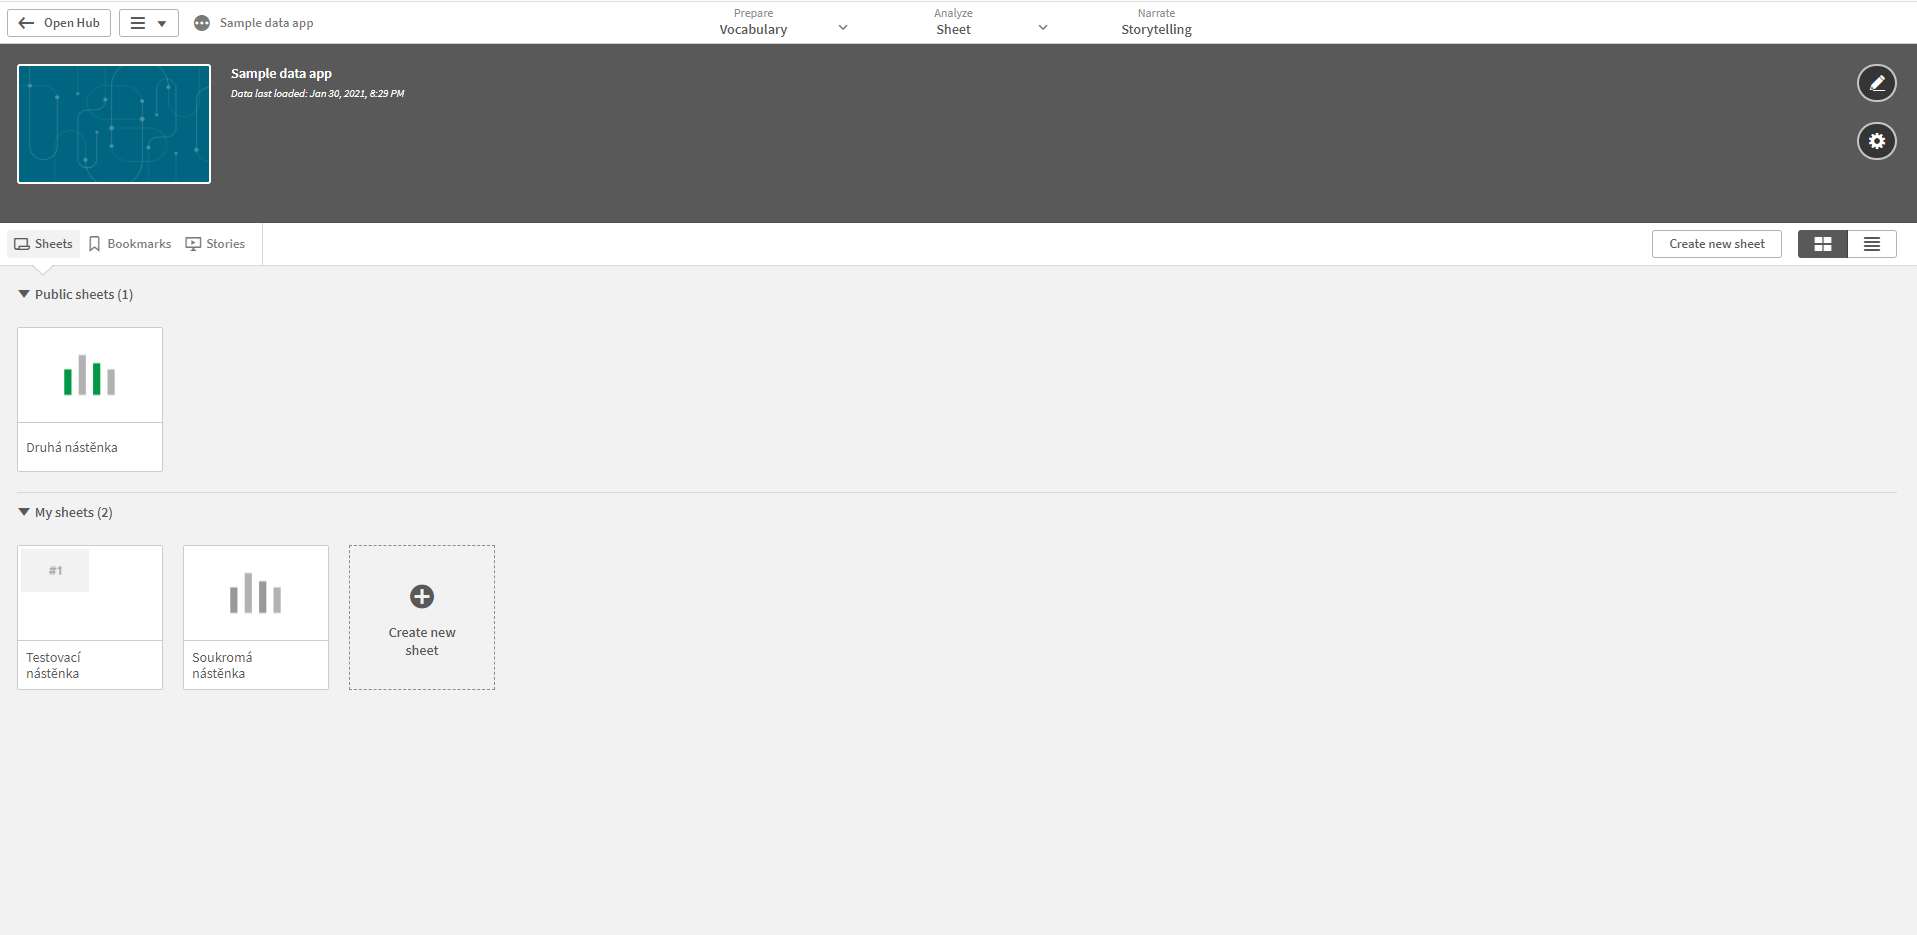
\includegraphics[width=1\textwidth]{Diplomka/Figures/qlik_project.png}
    \caption{Stránka projektu v~Qlik Sense}
    \label{fig:qlik_project}
\end{figure}


V~rámci uživatelského účtu je možno udržovat více projektů. Po zvolení určitého projektu se zobrazí detailní stránka daného projektu se seznamem nástěnek a prezentací. Tato stránka je zobrazena na obrázku \ref{fig:qlik_project}.  Ve vrchní vertikální navigaci se nacházejí tři oddělení:

\begin{itemize}
\item \textit{Prepare (příprava dat)} -- V~rámci tohoto oddělení je možno vybrat data, která se pro daný projekt budou používat.
\item \textit{Analyze (analýza a zobrazení dat)} -- Na této stránce se nacházejí nástěnky (položka \textit{Sheet}) a postřehy (položka \textit{Insights}). Stránka slouží pro zobrazení a analýzu dat.
\item \textit{Narrate} -- Na této stránce je pouze oddělení \textit{Storytelling}, pomocí něhož můžeme vytvořit prezentaci pro veřejnou prezentaci získaných dat.
\end{itemize}


Jak již bylo zmíněno, v~prvním oddělení je možno zobrazit datový model. To lze buď v~oddělení \textit{Data manager}, kde je zobrazení tabulek realizováno pomocí takzvaných bublin, které lze libovolně propojovat, nebo v~oddělení \textit{Data model viewer}, které zobrazuje tabulky podobně jako v~databázovém zobrazení. Dále se v~této záložce nachází \textit{Data load editor}, v~rámci něhož dokážeme nahraná data modifikovat a spravovat. Kromě správy dat lze v~záložce \textit{Prepare} upravovat byznys logiku pomocí logického modelu.

Na stránce s~postřehy (\textit{Insights})  si můžeme vložit nespočet různých vizualizací a sestav. Ty se dají pomocí levé navigace filtrovat. Následně můžeme zobrazovat různé sestavy, které je také možno vytvářet na základě nahraných dat. Jednotlivé sestavy lze přidat do nástěnek (\textit{Sheet}), kterých může být v~rámci projektu různý počet. Každou vizualizaci v~rámci sestavy na stránce \textit{Insights} lze kromě filtrování upravit nebo smazat. Na samotné nástěnce je sestava již pouze pro zobrazení. Stránku s~postřehy je možno vidět na obrázku \ref{fig:qlik_dashboard}. Nástěnky mohou být buď veřejné, kdy je vidí kdokoli, komu dáme odkaz, nebo soukromé.

\begin{figure}[!ht]
    \centering
    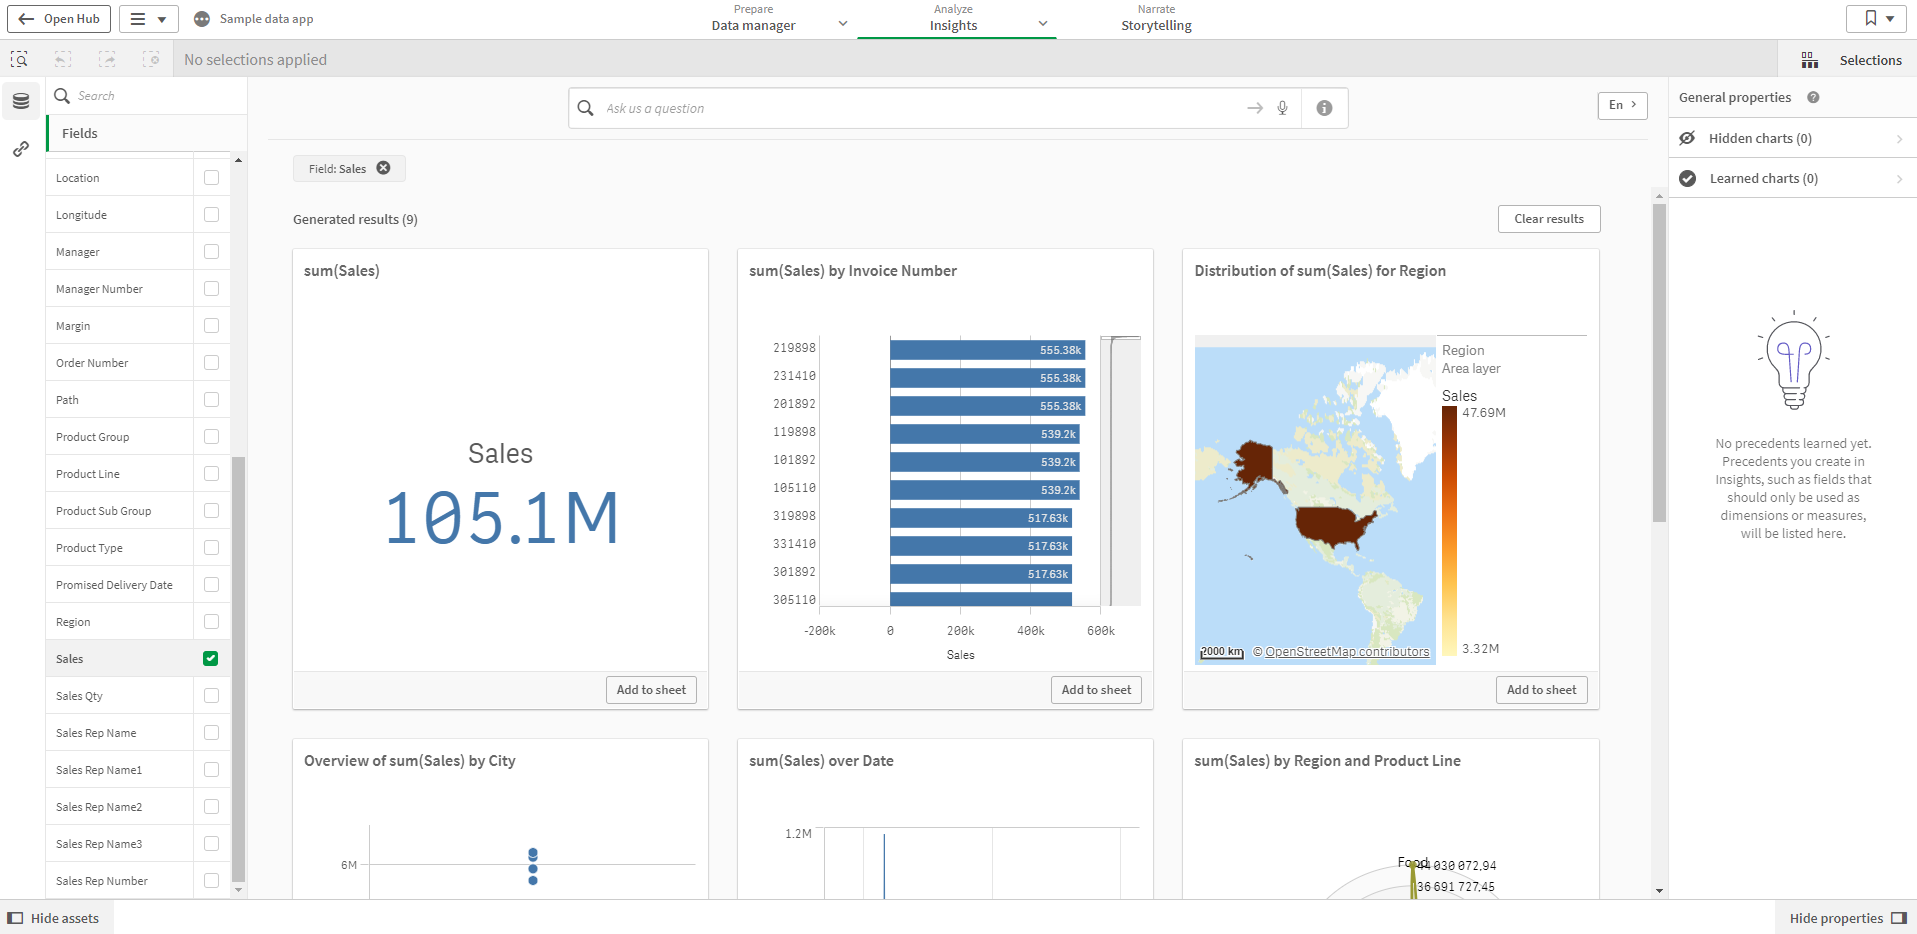
\includegraphics[width=0.93\textwidth]{Diplomka/Figures/qlik_dashboard.png}
    \caption{Nástěnka v~aplikaci Qlik Sense s~ukázkovými daty}
    \label{fig:qlik_dashboard}
\end{figure}

Poslední záložka s~názvem \textit{Storytelling} slouží pro prezentaci dat. Do prezentace je možno vložit prakticky jakákoli data, včetně jednotlivých nástěnek, na nichž se zobrazují živá a aktuální data. Tyto prezentace jsou stejně jako nástěnky buď veřejné, nebo soukromé.

V~rámci celého projektu je možno pomocí e-mailové adresy pozvat libovolný počet uživatelů, kteří na projektu pracují. Mezi hlavní výhody aplikace Qlik oproti konkurenčnímu Microsoft Power BI patří například našeptávání při realizaci vizualizací, existence průvodce, který uživatele učí jak s~aplikací pracovat. Další výhodou je možnost filtrovaní podobně jako v~klasických internetových vyhledávačích. Nevýhodou je značná komplikovanost ovládání a navigace v~rámci celé aplikace.

\section{Microsoft Power BI}
\label{sec:microsoft_power_bi}
Microsoft Power BI je komplexní platforma firmy Microsoft, jejímž cílem je poskytovat interaktivní vizualizace a funkce pro celé odvětví business intelligence. Veškeré tyto funkcionality jsou vymyšleny tak, aby byly pochopitelné a lehké na nastavení i pro začínající uživatele. Mezi základní funkcionality patří nástěnka a dále jednotlivé sestavy.

Aplikace je pro uživatele dostupná buď jako webová stránka nebo jako klasická počítačová aplikace pro operační systém Windows či jako aplikace pro mobilní zařízení. Dále existují varianty a licence pro různé další služby. Mezi ty patří například: \cite{ref:microsoft_bi_general}
\begin{itemize}
\item \textit{Embedded} -- pomocí REST API je možno vytvořit různé nástěnky a sestavy v~různých zařízeních a aplikacích mimo Microsoft Power BI.
\item \textit{Server sestav Power BI} -- služba poskytuje uživatelům přístup a následné generování různých sestav pomocí \textit{SQL Server Reporting Services}. Při vytvoření sestavy dokážou uživatelé vizuálně zkoumat data a díky tomu například provádět důležitá rozhodnutí.
\item \textit{Free} - verze zdarma, která je velmi omezená a neposkytuje například žádné sdílení sestav nebo nástěnek mezi uživateli Power BI.
\item \textit{Pro} -- jde o~levnější verzi licence s~omezenými službami a funkcionalitami oproti licenci \textit{Premium}. Aplikace je licencovaná na uživatele s~omezenými výpočetními prostředky, velikostmi datových sad, s~omezenou velikostí úložiště na jednotlivého uživatele a na sdíleném serveru společnosti Microsoft. Tato licence je obecně vhodná pro střední až velké podniky a společnosti, které mají menší objem dat potřebných k~analýze.
\item \textit{Premium} -- nejvyšší možná licence, která na rozdíl od verze \textit{Free} a \textit{Pro} není licencovaná na uživatele ale na celou organizaci. V~rámci této licence je pro celou organizaci vyhrazen prémiový prostor o~velikosti 100 TB. Dále licence poskytuje větší množství nástěnek a sestav. Taková licence je vhodná pro opravdu velké podniky a korporace.
\end{itemize}

Mezi hlavní výhody Microsoft Power BI patří zejména jednoduché napojení známých již existujících vývojových aplikací pomocí existujících doplňků, webová a mobilní aplikace nebo například rychlé vytváření přehledů a sestav. \cite{ref:microsoft_bi_general} Další velkou výhodou je automatické napojení na tabulkovou aplikaci Excel. Výhodou je intuitivnost ovládání podobně jako v~aplikacích Office, které jsou známy i mnoha začínajícím uživatelům. Mezi nevýhody můžeme zařadit menší možnosti exportu sestav a grafů do statických formátů, které je možné pouze do PDF. Na obrázku \ref{fig:powerbi_dashboard} je možno vidět definovanou sestavu společně s~vizualizovanými daty.

\begin{figure}[!ht]
    \centering
    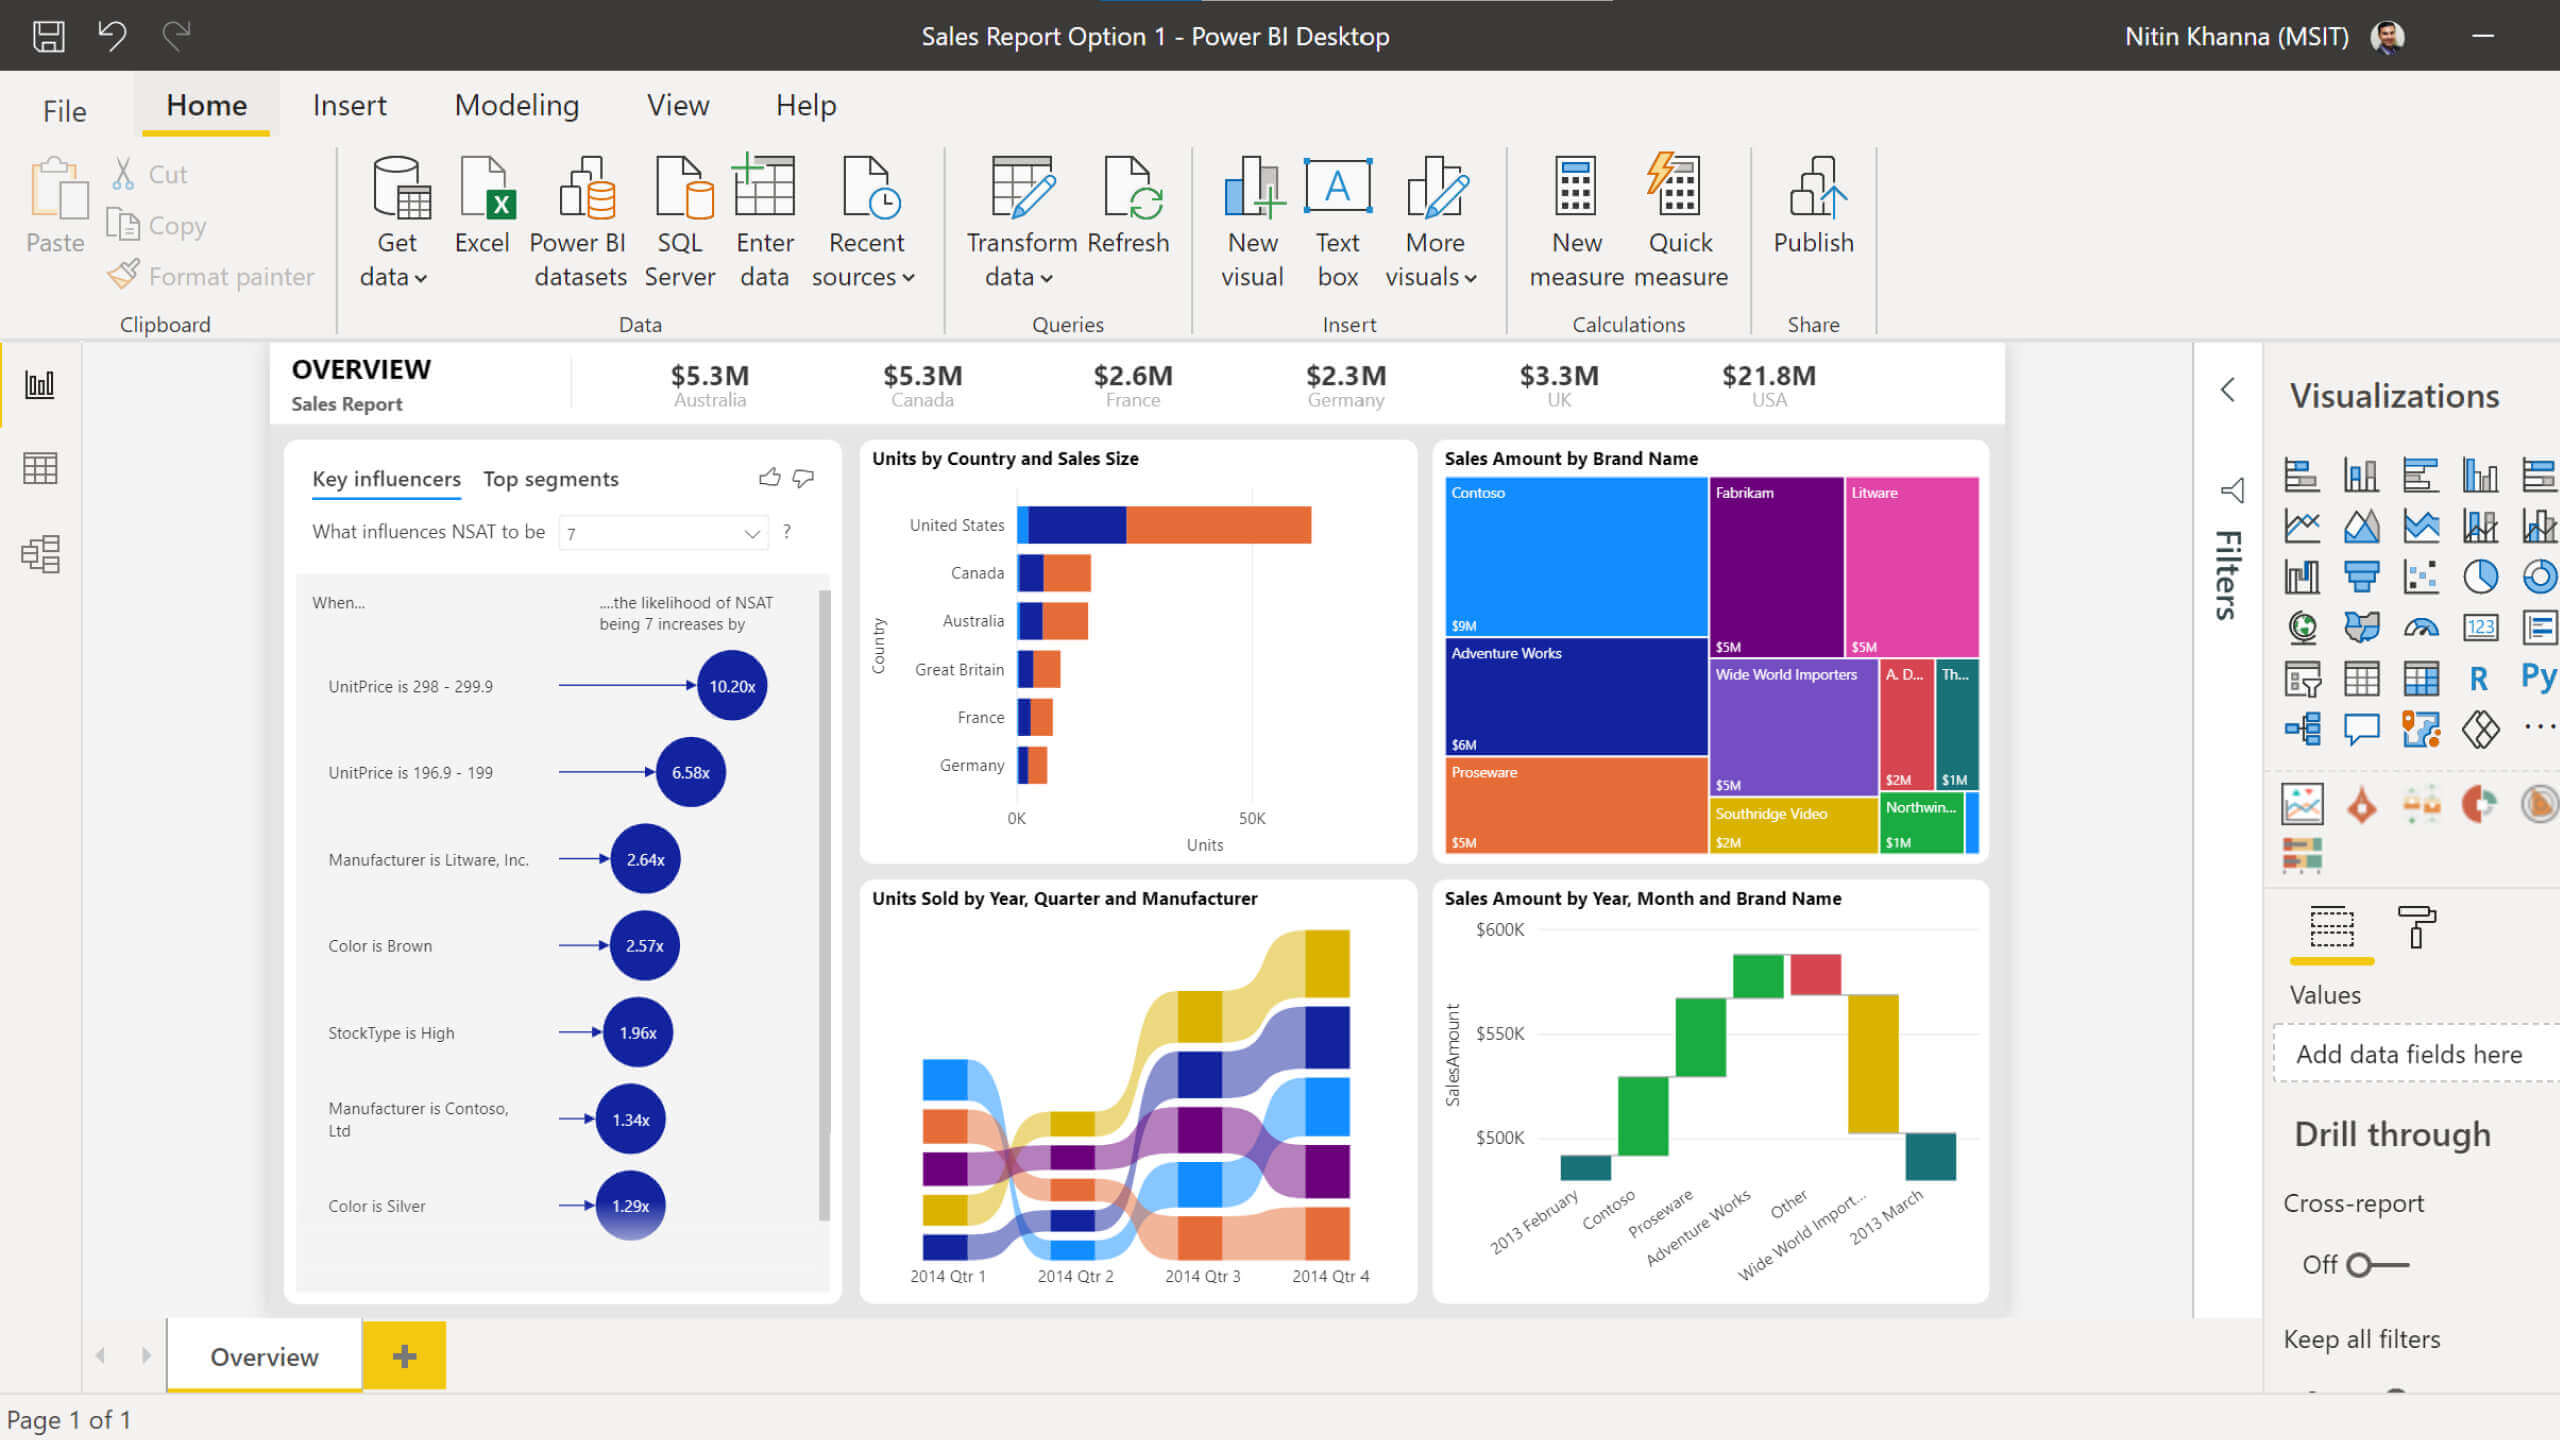
\includegraphics[width=1\textwidth]{Diplomka/Figures/powerbi-dashboard.jpg}
    \caption{Nástěnka v~aplikaci Microsoft Power BI (převzato z~\cite{ref:microsoft_bi_general})}
    \label{fig:powerbi_dashboard}
\end{figure}

Pro vytvoření sestavy jsou potřeba data. Ta lze vložit manuálně, vytvořit nebo zvolit existující datovou sadu. Data je možno exportovat z~různých, již existujících, systémů pro sběr a správu dat. Jakmile definujeme data, která chceme pro sestavu a \textit{report} použít, můžeme vybrat, jaká data chceme zobrazit ve kterém grafu. Aplikace Microsoft Power BI nabízí velké množství grafických vizualizací dat, což zlepšuje následné sledování a pochopení dat.


\chapter{Vlastní aplikace}
\label{sec:my_app}
V~rámci  praktické části této diplomové práce bylo potřeba vytvořit  prototypový nástroj pro sledování a zobrazování metrik potřebných pro splnění standardu Automotive SPICE. To znamená především definovat, vytvářet a sledovat metriky v~čase a následně vytvářet sestavy, které je možno exportovat do různých formátů. Základní vize byla, aby byl nástroj místem shromáždění dat a artefaktů z~platformy IBM Jazz v~čase. Hlavním důvodem pro vytvoření tohoto nástroje je, že platforma IBM Jazz a další podobné aplikace nepodporují sledování metrik potřebných pro splnění standardu Automotive SPICE. Zejména například generování trendových metrik v~určitém časovém období.

\section{Požadavky}
\label{sec:requirements}
Základním požadavkem pro aplikaci bylo, aby uživatel v~aplikaci mohl definovat a následně zobrazovat metriky v~čase. Nástroj bude umět definovat takové metriky, které jsou potřebné pro naplnění standardu Automotive SPICE. Dalším důležitým požadavkem bylo, aby aplikace byla realizována jako webová aplikace a byla tedy přístupná prakticky z~jakéhokoli zařízení. Aplikace bude nabízet role uživatelů, na něž budou navázány jednotlivé funkcionality nástroje. Přístup do nástroje bude mít pouze registrovaný uživatel.

Prototypový nástroj nebude obsahovat možnost zadávání dat pro samotné metriky -- tzn. sběry dat. Ty se budou automaticky, dle definovaného plánu, stahovat z~platformy IBM Jazz pomocí API nebo jinou automatickou extrakcí z~této platformy. Veškeré artefakty se budou importovat do projektů, které bude možno v~nástroji vytvářet. Dále se artefakty budou řadit do modulů stejně jako v~platformě IBM Jazz. Importovaná data se musí řadit a seskupovat dle data importu (tzv. sběru).

Aby bylo možno zajistit případné změny ve standardu Automotive SPICE, nebo dokonce i pouhou změnu potřeb měřit určité údaje, je potřeba, aby administrátor v~nástroji dokázal vytvořit definice metrik a z~těchto definic opakovaně různé metriky. Metriky bude možno poté přiřadit k~jednotlivým projektům. Metriky bude umět nástroj zobrazovat graficky a textově dle definovaných podmínek v~definici metriky. Grafické zobrazení metriky bude možné zobrazit buď na nástěnce, kterou si bude moct uživatel libovolně upravovat, nebo na detailním zobrazení dané metriky. Dále bude možno metriky exportovat do formátů PowerPoint a Excel. Grafické zobrazení v~aplikaci bude podporovat základní typy grafů, které bude možné filtrovat a měnit zobrazovaný rozsah dat na grafu.

Funkcionality celého nástroje lze rozdělit do funkčností, které ovládá uživatel, a dále funkčností, které provádí systém automaticky. Samotný uživatel může nabývat buď role administrátora, nebo normálního uživatele. Na obrázku \ref{fig:jazz_metrics_use_case} lze vidět grafické znázornění uživatelských případu užití. Tyto případy užití tedy ovládá uživatel.

\begin{figure}[!ht]
    \centering
    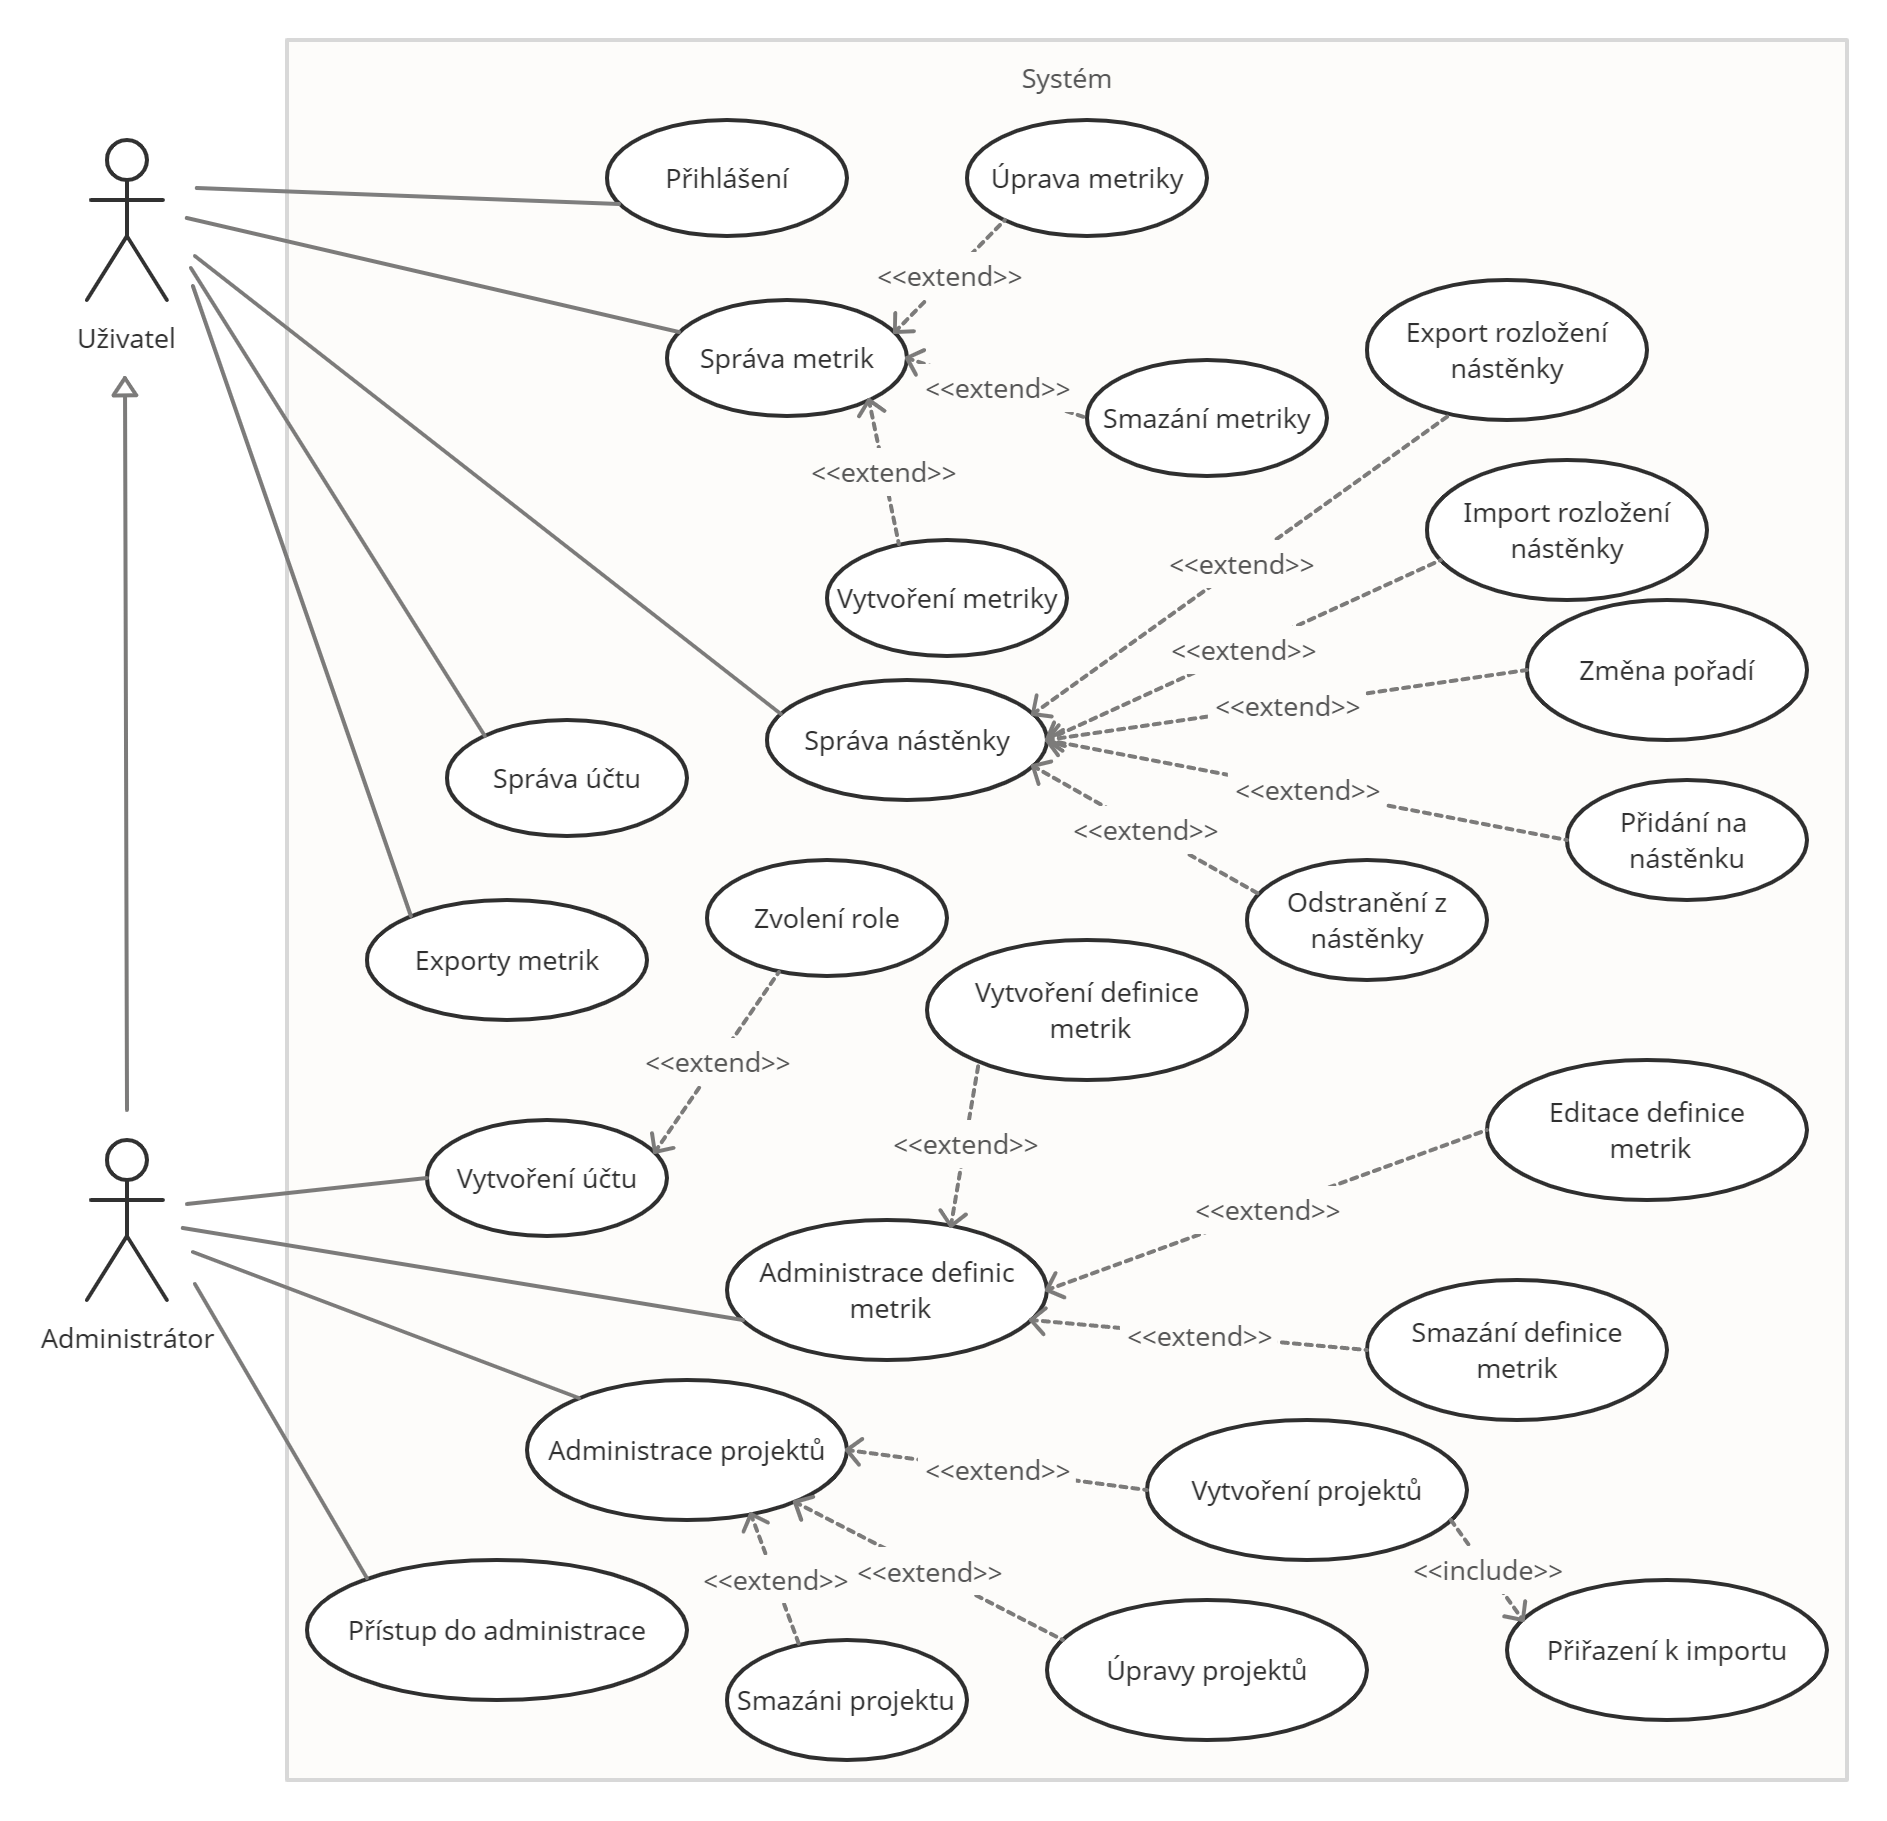
\includegraphics[width=0.95\textwidth]{Diplomka/Figures/use_case_jazz.png}
    \caption{Diagram případu užití vlastní aplikace pro metriky}
    \label{fig:jazz_metrics_use_case}
\end{figure}


Základním typem uživatele je klasický uživatel bez administrátorských práv. Kromě samozřejmosti v~podobě přihlášení může uživatel spravovat metriky. Tedy může metriky vytvářet, upravovat či případně mazat. Metriky může také pomocí speciálního nástroje v~podobě dokumentu exportovat do formátu PowerPoint a Excel. Uživatel může také vytvářet, upravovat, zobrazovat a exportovat dokumenty do různých formátů. Dokumenty slouží jako hromadné reporty (viz kapitola \ref{sec:reports}). Dále si může uživatel spravovat svůj účet a měnit různá nastavení. Každý uživatel má svou nástěnku, kterou si může libovolně spravovat. Kromě změny pozic jednotlivých metrik, přidávání a mazání metrik z~nástěnky může uživatel také exportovat nástěnku do formátu XML a poté ji sdílet například kolegovi pro samotný import nástěnky.

Uživatel s~právy administrátora má největší práva a přístup ke všem funkcionalitám, které nástroj nabízí. Kromě stejných funkcionalit jako běžný uživatel může administrátor využívat další funkčnosti celé aplikace. Administrátor může vytvářet ostatním uživatelům účty a přiřazovat jim jednotlivá práva a role. Důležitou funkcí administrátora je správa definic metrik. Pomocí těch administrátor může vytvářet, upravovat a mazat definice metrik, které poté používají uživatelé pro vytváření samotných metrik. Pomocí těchto definic je například poté možno vytvářet metriky v~souladu se standardem Automotive SPICE. Dále je požadováno, aby administrátor mohl vytvářet projekty, do kterých budou následně automaticky importovány jednotlivé artefakty z~platformy IBM Jazz. Import probíhá poté periodicky na pozadí celého nástroje dle definovaného rozvrhu v~CRON tabulce. Veškeré tyto funkcionality jsou přístupné přes administraci, kde má administrátor přístup.

\section{Architektura a použité technologie}
Vzhledem ke kladeným požadavkům na výsledný prototypový nástroj, které vyžadují, aby byl nástroj použitelný na jakékoli zařízení, bylo rozhodnuto, že nástroj bude realizován jako webová aplikace. Tento způsob je proti klasické klientské aplikace výhodnější v~několika ohledech. Největší výhodou je nezávislost platformy, na které je nástroj provozován. Uživatel nemusí kromě webového prohlížeče instalovat žádnou další aplikaci potřebnou pro běh nástroje. Dalším kladem je jednodušší správa a aktualizace celého nástroje. Nástroj bude do budoucna připraven na vytvoření progresivní webové aplikace. Celá aplikace je v~souladu s~architekturou Model-View-Controller.

Architektura se skládá z~několika důležitých komponent a vrstev. Celou architekturu systému včetně napojení na platformu IBM Jazz je možno vidět na obrázku \ref{fig:architektura_nastroje}. Nejvyšší vrstvou nástroje je prezentační vrstva sloužící zejména pro komunikaci mezi uživatelem a celým nástrojem. Uživatel pomocí prezentační vrstvy nástroj ovládá a provádí různé úkony vedoucí k~vytvoření projektů, metrik nebo například definicí metriky. Veškeré tyto úkony jsou definovány v~kapitole \ref{sec:requirements}. Celý nástroj je ovládán pomocí grafického uživatelského rozhraní ve webovém prohlížeči. Tuto vrstvu řadíme v~architektuře Model-View-Controler k~\textit{View}. Prezentační vrstva je realizována pomocí šablonovacího systému Twig.

Další vrstvou je aplikační vrstva, která vykonává většinu aplikační logiky, kontroluje vstupy od uživatele, provádí výpočty a zpracovává data. Tato vrstva je provozována pomocí frameworku Symfony v~jazyce PHP. Této technologii je podrobněji věnována kapitola \ref{sec:symfony}. V~této vrstvě jsou zahrnuty veškeré kontrolery, které komunikují s~prezentační vrstvou, z~níž přijímají data a pokyny od uživatele. Dále do této vrstvy můžeme zařadit jednotlivé modely, které přistupují k~datové vrstvě. Komunikace mezi datovou a aplikační vrstvou probíhá pomocí repositářů. V~rámci přístupu k~repositářům je použit návrhový vzor fasáda z~důvodu uceleného přístupu k~datům a repositářům.

Vrstva, kterou je možno považovat i za aplikační vrstvu, je servisní vrstva, která zajišťuje automatické stahování dat z~platformy IBM Jazz. Stahování dat, zejména artefaktů, probíhá pro definované projekty pomocí \textit{Cron} modulu. Toto stahování probíhá na pozadí dle definovaného času spuštění. Stažení dat je možno vyvolat také z~příkazové řádky. Dále je k~dispozici v~případě potřeb jednoduchá a pohodlná možnost přidat zavolání a spuštění servisního modulu pomocí prezentační vrstvy.

Další nedílnou součástí celého nástroje je datová vrstva. Tato část komunikuje s~aplikační vrstvou pomoci již zmíněných repositářů. Datová vrstva ve skutečnosti používá dvě různé technologie pro ukládání dat. Prvním používaným úložištěm je relační databáze PostgreSQL, která slouží zejména pro ukládání uživatelů a uživatelských rolí. Tato technologie byla zvolena pro tento účel zejména pro bezpečné a rychlé ukládání hesel, dat uživatelů a jednotlivých uživatelských rolí. Objekty namapované na relační databázi jsou nazývány entity. Druhým používaným úložištěm je \textit{NoSQL} databáze MongoDB. V~tomto úložišti je uložena drtivá většina dat celého nástroje. Jsou zde uloženy například veškeré definice metrik, metriky, artefakty, nástěnky a další uživatelská data. Tato technologie byla zvolena po konzultaci s~vedoucím práce díky vlastnostem lépe a pohodlněji ukládat celé objekty, rychlosti a lepší správě většího počtu dat. Tohoto benefitu bylo využito zejména při ukládání velkého množství artefaktů. Další velkou výhodou této technologie je možnost pohodlné správy celé struktury databáze. Velkou výhodou využití technologie MongoDB bylo při ukládání artefaktů a definic metriky to, že celá struktura objektů je tvořena pomocí vnořených či případně propojených objektů což umožňuje jednodušší a pohodlnější dotazování na objekty. Jednotlivé objekty jsou nazývány dokumenty.



\begin{figure}[!ht]
    \centering
    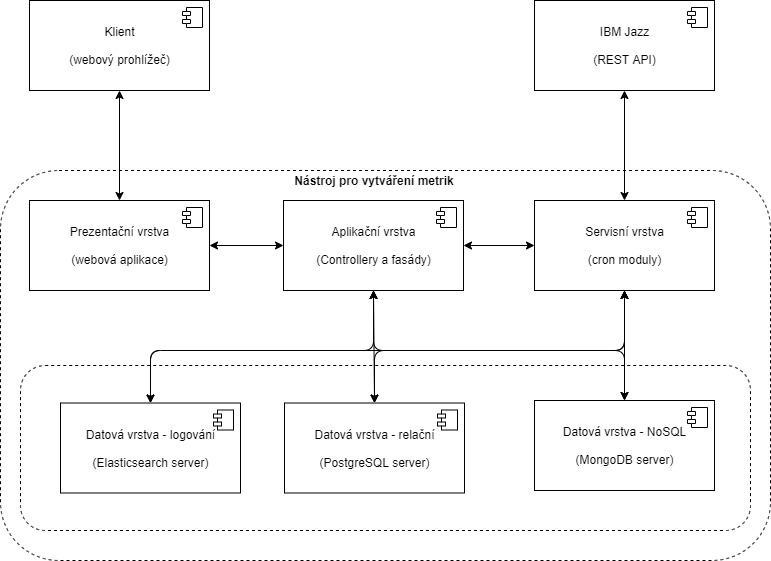
\includegraphics[width=1\textwidth]{Diplomka/Figures/architektura.png}
    \caption{Architektura nástroje pro vytváření metriky}
    \label{fig:architektura_nastroje}
\end{figure}


Celou aplikaci je možno provozovat buď nativně přímo na operačním systému, nebo pomocí technologie Docker. Při instalaci nativní je nutno nainstalovat veškeré závislosti, které nástroj využívá. Mezi takové závislosti můžeme zařadit například relační a NoSQL databázi, přesnou verzi PHP, webserver a mnoho dalších. Pro pohodlnější a jednodušší instalaci je vhodné použít virtualizačního nástroje Docker. Výhodou použití této technologie je, že aplikace je nasazena v~produkčním, testovacím a vývojovém prostředí na stejných verzích závislostí a podpůrných nástrojů. V~rámci instalace pomocí Dockeru se nainstaluje i nástroj Kibana a NoSQL databáze Elasticsearch pro správu všech logů aplikace. Dále se nainstalují nástroje jako například Adminer pro správu databází,  Mongo-gui pro grafickou vizualizaci dokumentů v~MongoDB databázi a další. Technologii Docker a použití využívaných nástrojů se věnuje kapitola \ref{sec:docker}.

\subsection{Symfony}
\label{sec:symfony}
Základním kamenem celého nástroje pro správu metrik je framework Symfony. Ten je vytvořen na skriptovacím jazyce PHP. Aplikace je schopna běžet na PHP od verze 7.4 a výše, tedy nejnovějších a podporovaných verzích. Symfony používá plně objektového přístupu a aplikace dále využívá veškerých moderních funkcionalit skriptovacího jazyka PHP pro kontrolu datových typů. Jednotlivé metody a proměnné jsou datově typovány a datové typy pečlivě kontrolovány. Framework Symfony je využíván v~nejnovější verzi 5.2. Jelikož Symfony vychází z~frameworku Spring jazyku Java, je práce a vývoj prakticky identický. Práce je podobná i přesto, že jazyk PHP je skriptovací, jelikož je silně vyžadováno deklarování datových typů a jejich následná kontrola. Kontrola je také podpořena automatickými testy a kontroly standardů. Aplikace funguje na architektuře MVC, přičemž je plně připravena místo samotných kontrolerů používat API \textit{endopointy} a prezenční vrstvu vykreslovat pomocí technologie JavaScript. Celá aplikace využívá velké množství mezipaměti, což vede k~vyšší rychlosti celé aplikace. Samotnou aplikaci dokážeme zrychlit při použití nového PHP 8, využívající \textit{just-in-time} kompilaci.

Důvodey zvolení technologie Symfony a PHP místo technologie Spring nebo ASP.NET byly zejména modernost celé platformy, menší náročnosti na server, velké komunity vývojářů a rychlosti odezvy celého systému. Dalším benefitem byla zkušenost vývoje opravdu velkých aplikací v~tomto frameworku. Jelikož je jazyk PHP nejpoužívanějším jazykem spouštěným na serveru, nabízí velké množství dokumentace a podpory. \cite{ref:php_trend} Velkou výhodou je i počet vývojářů, kteří jazyk PHP znají.  V~případě použití nových verzí 7.4, nebo 8 nemusí být jazyk tak velkou potíží. Nevýhodou je špatná reputace jazyku PHP jako takového a případná reputace nevhodnosti použití pro velké podnikové aplikace. Další nevýhodou může být možnost špatného psaní kódu a nerespektování veškerých standardů a datových typů. Tato nevýhoda lze, stejně jako v~této práci, podchytit automatickou kontrolou a opravou standardů.

\subsection{Datová vrstva}
Tato vrstva slouží k~ukládání dat z~celé aplikace. Jak již bylo nastíněno, v~aplikaci existují dva typy úložiště:

\begin{itemize}
\item relační databáze PostgreSQL,
\item NoSQL databáze MongoDB.
\end{itemize}

Relační databáze je používána pro základní funkcionality aplikace, zejména pro správu uživatelských účtů a uživatelských rolí. Dále je tato databáze používána pro ukládání informací seznamu a informací o~běhu modulů servisní vrstvy. Relační databáze je realizována pomocí PostgreSQL. Jednotlivé tabulky jsou realizovány jako entity, které se automaticky mapují na databázové tabulky. Aby byla zajištěna synchronizace a vytváření jednotlivých tabulek mezi všemi vývojáři případně při nové instalaci, je používáno takzvaných migrací. Migrace si můžeme představit jako jednotlivé soubory obsahující SQL dotazy pro vytvoření či úpravu tabulek.

Hlavním datovým úložištěm celého nástroje je NoSQL databáze MongoDB. V~této databázi jsou uložena veškerá data související s~metrikami, projekty, artefakty a vším ostatním. Přípojení k~MongoDB je možno používat buď v~rámci balíčku Docker, nebo využitím cloudové licence přímo na serverech společnosti MongoDB Inc. Jednotlivé objekty této databáze jsou pojmenovány jako dokumenty. Tyto dokumenty nejsou ve všech případech, jako v~relační databázi, spojeny pomocí klíčů, ale jsou také vnořeny. Druhým případem propojení je pomocí odkazu na jiný dokument. Největší výhodou vnořování dokumentů je to, že data jsou prakticky součástí jednoho dokumentu, což ulehčuje dotazování a vkládání do databáze. Dokumenty uložené v~databázi MongoDB je možno vidět na obrázku \ref{fig:mongo_diagram}.

Na diagramu můžeme vidět dvě základní sekce Metriky a Artefakty. V~rámci sekce obsahující dokumenty související s~metrikami se nachází například dokument \texttt{metricDefinitions}. V~tomto dokumentu jsou uloženy veškeré definice metrik,v rámci kterých jsou ve vnořených dokumentech podmínky pro vytvoření dané metriky. Dále se zde nachází dokument pro samotné metriky, které jsou vázány jak na projekty, tak i na moduly, z~nichž čerpají data. Každá metrika má zvolený typ grafu a může patřit do různých rozvržení nástěnky, která existují vždy pro každého registrovaného uživatele. Tyto vazby jsou řešeny pomocí  referencí, což je obdoba cizích klíčů pro relační databázi.

\begin{figure}[!ht]
    \centering
    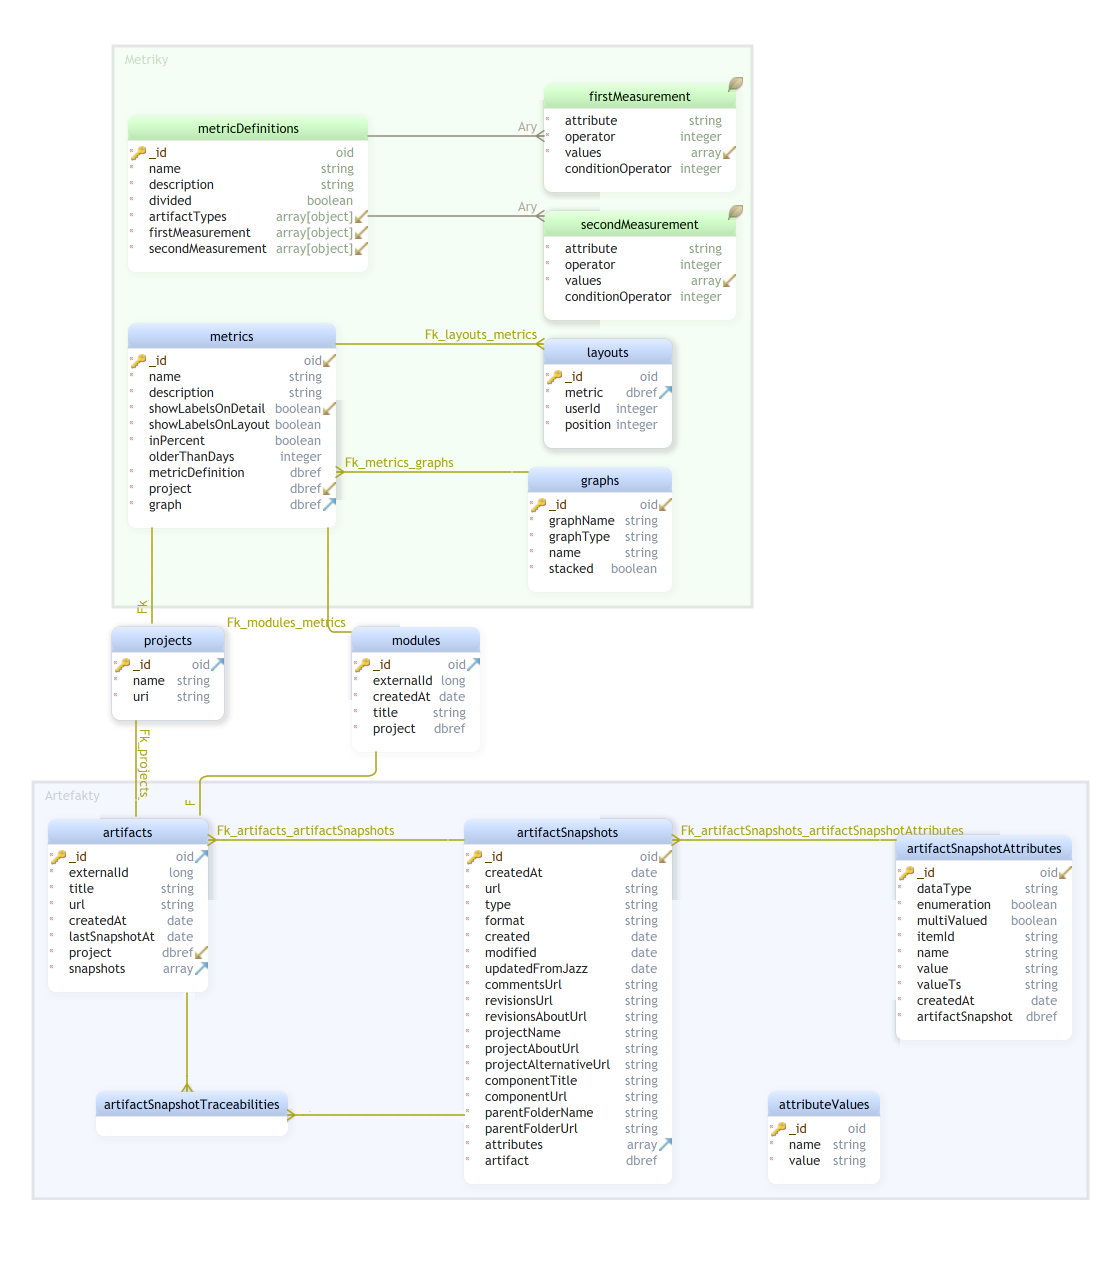
\includegraphics[width=1\textwidth]{Diplomka/Figures/db_diagram.png}
    \caption{Diagram části NoSQL MongoDB databáze pro ukládání artefaktů a metrik}
    \label{fig:mongo_diagram}
\end{figure}
Následně existuje v~aplikaci druhá sekce, která seskupuje dokumenty zabývající se artefakty. V~této sekci je nejdůležitějším dokumentem \texttt{artifacts}, který udržuje veškeré artefakty stažené z~platformy IBM Jazz. Jednotlivé artefakty mají \texttt{artifactSnapshots}, které uchovávají verze v~den daného stažení artefaktu. Zároveň mají tyto artefakty jednotlivé atributy a případně propojení s~ostatními artefakty. V~jednotlivých verzích a jejich atributech se nachází veškerá důležitá data pro generování hodnot definovaných metrik. Také zde existuje dokument \texttt{attrbiteValues}, který slouží pouze jako dokument s~agregovanými daty pro rychlejší načítání formuláře pro definice metrik. Veškerá propojení jsou realizována pomocí referencí z~důvodu vytváření dotazů a získávání dat pro vykreslování metrik. Artefakty jsou dále propojeny pomocí referencí s~projekty a moduly. Veškeré informace se stahují automaticky z~platformy IBM Jazz.

Pro oba typy úložiště je používán ORM framework Doctrine, který je ve výchozím stavu součástí Symfony. Slouží pro komunikaci mezi aplikací a databázemi. Framework Doctrine se skládá z~abstraktní databázové části  a ORM části. Abstraktní část slouží pro připojení k~různým typům databází a také zajišťuje základní přístupy a metody pro práci s~databázemi. ORM část má na starost mapování objektů v~aplikační části na databázový objekt a zpět. Framework Doctrine používá pro mapování objektů návrhový vzor \textit{data mapper}.


Dále v~aplikaci existuje třetí typ úložiště -- Elasticsearch. Toto úložiště slouží pouze pro ukládání logů, neslouží pro ukládání samotných dat aplikace. Tato data je poté možno jednoduše zobrazit v~aplikaci Kibana, která logy shromažďuje a pomocí níž lze v~lozích hledat a filtrovat.

\subsection{Docker}
\label{sec:docker}
Je to open-source nástroj, pomocí něhož můžeme vytvořit jednotné rozhraní pro instalaci aplikace. Docker nám zajišťuje, že ač nasadíme aplikaci na různé operační systémy, tak nám vytvoří stejné definované prostředí. Oproti klasickým virtuálním strojům Docker kontejner neobsahuje virtualizovaný operační systém. Tím je výrazně snížena náročnost a rychlost celé funkčnosti oproti klasickým virtuálním strojům. S~tím souvisí i menší velikost a nižší náklady na provoz než celý virtuální stroj. Nevýhodou Linuxových kontejnerů je horší podpora na operačních systémech Windows a macOS.

Docker je v~rámci prototypového nástroje použit právě na vytvoření vývojového a produkčního prostředí. Do Docker kontejneru se tedy instalují všechny potřebné závislosti, které jsou pro běh nástroje potřebné. V~rámci hlavního konfiguračního souboru se nainstalují závislosti jako správná verze PHP, PostgreSQL, MongoDB a mnoho dalšch. Dále existují samostatné konfigurační soubory pro webový server a Elasticsearch. Tyto konfigurační soubory nazývané \textit{Dockerfile} se pomocí nástoje \textit{Docker Compose} spojí a vytvoří jeden spustitelný kontejner. Na výpisu kódu \ref{src:docker_compose} můžeme vidět malou část konfiguračního souboru \textit{docker-compose.yml}, pomocí kterého vytvoříme a nainstalujeme závislost pro PostgreSQL databázi.

\lstinputlisting[label=src:docker_compose,caption={Část konfiguračního souboru docker-compose.yaml sestavující PostgreSQL}, language=xml]{SourceCodes/docker-compose.yml}

Největší výhoda tkví v~jednodušší instalaci, jelikož stačí nainstalovat pouze Docker a veškeré závislosti se doinstalují do kontejneru samy. Dále můžeme jednoduše spravovat a povyšovat verze všech závislostí. Jelikož všichni potencionální vývojáři mají stejné vývojové a následně produkční prostředí, nedochází k~nesrovnalostem mezi vývojovým, testovacím a produkčním prostředím. Aplikace samozřejmě může běžet bez Dockeru nativně přímo na systému. Poté je ale nutno zajistit stejné verze všech závislostí a případně je manuálně povyšovat dle potřeb.



\section{Export dat z~IBM Jazz}
\label{sec:ibm_export}

Jednotlivá data a artefakty se nevytvářejí v~prototypovém nástroji pro sledování metrik, ale importují se a stahují z~platformy IBM Jazz. Tyto požadavky a artefakty je tedy nutno nejprve vložit do platformy IBM Jazz. Artefakty je vhodné zařadit do modulů dle jejich oblasti. V~rámci Automotive SPICE můžeme mezi takové moduly zařadit například hardwarové požadavky se zkratkou HWRS. Používání těchto modulů je vhodné pro následné vytváření metrik a selekci pouze určitých typů artefaktů.

Pro stahování dat z~platformy IBM Jazz je možno použít několik druhů napojení. V~rámci této kapitoly budou možná napojení analyzována a bude vybráno právě jedno, které bude následně v~rámci praktické části použito pro export do prototypového nástroje.

\subsection{Manuální export do CSV}
Jde o~nejprimitivnější možnost exportu jednotlivých artefaktů. Tuto úlohu nelze nijak jednoduše a elegantně automatizovat. Export může vyvolat pouze přihlášený uživatel s~povolenými přístupy k~artefaktům. Export je možno vyvolat buď na stránce s~výpisem všech artefaktů, nebo na stránce s~výpisem pouze určitých artefaktů (například při zobrazení jen daného modulu), popřípadě také na detailu pouze jednoho artefaktu.

Výhoda tohoto exportu spočívá v~jeho jednoduchosti. Následné zpracování CSV je poté také nenáročné na implementaci. Výhodou je, že do CSV je možno vložit prakticky jakékoli údaje až na propojení s~ostatními artefakty. Naproti tomu velkou nevýhodou je nemožnost tento proces automatizovat. Vždy by musel existovat uživatel, který CSV vygeneruje a nahraje do nástroje pro generování metrik. Z~tohoto důvodu je tento export prakticky pro pravidelné aktualizace nepoužitelný.

\subsection{Reportable REST API}
Toto API, jak již název napovídá, funguje na principu architektury REST. Reportable REST API slouží pouze pro export z~nástroje konfiguračního managementu, neboli na platformě IBM Jazz pojmenované jako Change and Configuration Management (CCM). Tento nástroj bohužel neobsahuje žádné artefakty a požadavky a slouží zejména pro správu projektu a zdrojového kódu.

Abychom získali data z~tohoto API, je nutno nejprve provést autentifikaci. Po úspěšné autentifikaci lze data získat pomocí HTTP metody GET. Ta nám vrátí XML s~položkami konfiguračního managamentu. Data vrácená ve formátu XML lze poté jednoduše zpracovat a uložit do vlastní databáze. Pomocí speciálních parametrů v~HTTP metodě je možno data filtrovat. Jelikož však API neslouží pro data z~oblasti správy požadavků, nemůže být pro prototypový nástroj použito.

\subsection{Process REST API}
Jde o~provizorní a testovací API vyvíjené IBM, které se může dle dokumentace v~budoucnosti změnit. Slouží zejména pro export informací o~projektech. API funguje na principu REST a můžeme jej tedy  zavolat pomocí klasických HTTP GET a POST metod. Slouží nejen pro export dat, ale i pro import dat do platformy IBM Jazz. V~rámci API dokážeme zjistit údaje o~uživatelích pracujících na projektu, administrátory, moduly daného projektu, role a další. Bohužel na školním serveru s~nainstalovaným IBM Jazz nebylo toto API k~dispozici a nebylo tedy možno otestovat všechny vlastnosti. Velkou nevýhodou je, že API je pouze provizorní a může se v~budoucnu změnit. Další nevýhodou je, že pravděpodobně dle dokumentace neobsahuje podrobné informace o~artefaktech.

\subsection{Work Items Service provider for OSLC 2.0 CM}
Toto API poskytuje pomocí technologie Open Services for Lifecycle Collaboration (OSLC) ve verzi 2 přístup skoro ke každé informaci vyskytující se na platformě IBM Jazz. Koncepce OSLC je založena na tom, že webová stránka je přístupná jak pomocí HTML, tak i pomocí formátu RDF, který je jednoduše strojově čitelný. Přístup k~formátu RDF je stejně jako k~HTML dostupný pomocí protokolu HTTP.

Napojení pomocí OSLC je velmi komplexní a nabízí velké množství informací z~prakticky všech aplikací platformy IBM Jazz. Autorizace k~API probíhá pomocí speciální HTTP metody. Přístup k~jednotlivým datům je řešen pomocí různých HTTP metod. Při volání určité HTTP metody je možno data filtrovat pomocí parametrů. Kromě filtrování můžeme pomocí parametrů data stránkovat. Výhodou je, že nemusíme mít v~naší aplikaci definovány jednotlivé URL, ale stačí jedna základní, jelikož program se k~výsledné metodě může dostat sám díky struktuře RDF. Výsledky je možno kromě formátu XML zobrazit také ve formátu JSON.

Toto napojení jsem podrobně testoval a zkoušel na školním serveru s~nainstalovanou platformou IBM Jazz. Pomocí tohoto napojení můžeme jednoduše získat jednotlivé artefakty v~projektu, informace o~projektech, modulech v~projektu, uživatelích a velké kvantum dalších informací. Ač napojení nabízí obrovské množství informací a dat, pro využití stahování dat do našeho prototypového nástroje je nevhodné, jelikož nenabízí zevrubné informace o~vlastních atributech artefaktu. Napojení bohužel nabízí pouze základní atributy, nenabízí možnost stáhnout uživatelsky definované atributy a propojení artefaktů s~jinými artefakty.

\subsection{DOORS Next Generation Rest API}
Přístup k~datům pomocí tohoto API probíhá pomocí HTTP metod na architektuře REST. Napojení nabízí export dat z~nástroje IBM Engineering Requirements DOORS Next. Ten obsahuje zejména artefakty, které jsou v~projektech řazeny do modulů a adresářů. Pomocí napojení dokážeme exportovat veškeré atributy artefaktů včetně napojení na ostatní artefakty. Mezi atributy, které lze exportovat, patří i veškeré uživatelsky definované atributy.

Autorizace připojení k~API probíhá pomocí speciální metody, která nám vrátí \textit{cookies}, jež se uloží do mezipaměti a slouží pro následný dotaz. Data získáváme ve formátu XML po dotazu na definované URL. Pomocí parametrů v~URL můžeme výsledky filtrovat a stránkovat. Stejně jako v~případě jiných REST API dokážeme tuto činnost automatizovat. Mezi další výhody patří to, že API poskytuje veškeré údaje a data, které potřebujeme pro sestavení metrik. Jedinou nevýhodou může být špatná dokumentace, která neobsahuje veškeré metody. Ty je nutno hledat na různých internetových diskuzních fórech.

\subsection{Napojení na databázi}
Tento způsob můžeme zařadit k~nejzazšímu možnému způsobu exportu dat. Způsob lze využít pro export prakticky jakýchkoli typů dat. Jelikož platforma IBM Jazz používá pro ukládání dat relační databázi, můžeme pro export dat z~platformy využít SQL dotazy. Plusem této metody je, že proces můžeme zautomatizovat. Další výhoda způsobu exportu dat přímo z~databáze spočívá v~tom, že můžeme získat při znalosti architektury databáze prakticky jakákoli data. S~tím však souvisí velká nevýhoda, a to znalost struktury a architektury celé databáze, která je velmi komplexní. Další nevýhodou je, že ne vždy můžeme přístup k~databázi získat. K~datům nemusíme mít například přístup při používání platformy IBM Jazz v~cloudu. Existuje zde i pravděpodobnost, že při aktualizaci platformy Jazz dojde ke změně struktury databáze a tím může přestat správně fungovat export dat.

\subsection{Porovnání}
Platforma IBM Jazz nabízí velké množství možností pro export dat. Jelikož většina z~nich je zastaralá, nebyla v~rámci této kapitoly ani zmíněna. Některé stále podporované možnosti jsou z~hlediska přístupu modernější a některé starší a je pravděpodobné, že budou v~budoucnosti zrušeny. Většina analyzovaných možností je bohužel nevyhovující ať už z~toho důvodu, že nepodporují export dat, která potřebujeme pro definici metrik, nebo z~důvodu nemožnosti automatizace celého procesu. V~tabulce \ref{tab:ibm_jazz_export} jsou přehledně zmíněny vlastnosti a kritéria exportu dat:

\begin{enumerate}
\item možnost automatizace,
\item možnost exportu artefaktů,
\item možnost exportu uživatelských atributů artefaktů,
\item filtrování,
\item moderní a udržitelný přístup.
\end{enumerate}

\begin{table}[htp]
\centering
\begin{tabular}{@{}llllllll@{}}
\toprule
 & \textbf{Vlastnost}                          & \textbf{1} & \textbf{2} & \textbf{3} & \textbf{4} & \textbf{5} &  \\ \midrule
 & Manuální export do CSV                      & ne         & ano        & ano        & ne         & ne         &  \\
 & Reportable REST API                         & ano        & ne         & ne         & ano        & ano        &  \\
 & Process REST API                            & ano        & ne         & ne         & ano        & ano        &  \\
 & Work Items Service provider for OSLC 2.0 CM & ano        & ano        & ne         & ano        & ano        &  \\
 & DOORS Next Generation Rest API              & ano        & ano        & ano        & ano        & ano        &  \\
 & Napojení na databázi                        & ano        & ano        & ano        & ano        & ne         &  \\ \bottomrule
\end{tabular}
\caption{Porovnání analyzovaných možností exportu dat z~IBM Jazz}
\label{tab:ibm_jazz_export}
\end{table}

Na základě porovnání vychází, že ideálním nástrojem pro automatické stahování dat z~platformy IBM Jazz je  DOORS Next Generation Rest API, které kromě horší dokumentace nabízí veškeré vlastnosti, které jsou potřeba pro stahování dat, z~nichž se budou definovat a vytvářet metriky. Pakliže by neexistoval požadavek na pokročilé stahování uživatelských atributů artefaktů, jeví se jako lepší řešení Work Items Service provider for OSLC 2.0 CM, jelikož nabízí lépe zdokumentované metody. Dále je možno veškeré informace stahovat rovnou z~databáze celé platformy IBM Jazz. Tento způsob je však neperspektivní a hrozí, že kdykoli se databáze změní, stahování dat přestane fungovat.

\section{Stahování a ukládání dat}
Na základě výsledků analýzy v~kapitole \ref{sec:ibm_export} byl vybrán export dat pomocí IBM Jazz je  DOORS Next Generation Rest API. Aby bylo zajištěno pravidelné stahování dat z~REST API, byl vytvořen cron modul, který je možno spouštět pravidelně v~definované periodě. Tento skript stahuje data pro veškeré definované projekty v~prototypovém nástroji z~nastavené URL k~platformě IBM Jazz.

Jakmile si skript stáhne XML s~daty artefaktů pro daný projekt, vytvoří z~jednotlivých elementů objekt typu \textit{RmArtifact}, který obsahuje veškeré údaje získané z~XML souboru. Tyto objekty slouží jako datové objekty, které se poté namapují na konečné aplikační objekty, a ty se uloží do databáze. Aby bylo zajištěno co nejefektivnější, nejsrozumitelnější a nejrychlejší stahování a čtení XML souboru, byly provedeny dva prototypy, na kterých byla ověřena rychlost čtení. Pro čtení artefaktů z~XML souboru byly vybrány čtyři základní techniky:

\begin{enumerate}
\item iterování a procházení elementů (i vnořených) pouze pomocí XPath,
\item iterování a procházení jednoduchých elementů pomocí XPath a procházení složitějších elementů pomocí objektů \textit{SimpleXMLElement},
\item iterování pomocí cyklu a objektů \textit{SimpleXMLElement} a procházení vnitřních elementů pomocí XPath,
\item iterování pomocí cyklu a objektů \textit{SimpleXMLElement}.
\end{enumerate}

Výsledky měření těchto čtyř algoritmů se nacházejí v~následující tabulce \ref{tab:xml_read} a graficky v~grafu na obrázku \ref{fig:xml_read_plot}:

\begin{table}[htp]
\centering
\begin{tabular}{@{}ccccc@{}}
\toprule
\textbf{Pokus} & \textbf{Algoritmus 1} & \textbf{Algoritmus 2} & \textbf{Algoritmus 3} & \textbf{Algoritmus 4} \\ \midrule
1                 & 30,122                & 26,909                & 24,321                & 18,324                \\
2                 & 25,124                & 17,845                & 21,897                & 16,940                \\
3                 & 24,789                & 19,285                & 20,214                & 15,111                \\
4                 & 29,323                & 25,002                & 23,875                & 17,369                \\
5                 & 35,478                & 20,783                & 19,811                & 16,989                \\
6                 & 32,989                & 21,154                & 18,237                & 20,535                \\
7                 & 27,324                & 18,369                & 27,412                & 20,237                \\
8                 & 26,668                & 23,423                & 24,217                & 18,770                \\
9                 & 29,782                & 17,998                & 26,211                & 17,315                \\
10                & 28,369                & 20,312                & 19,996                & 16,732                \\ \midrule
Průměrně          & 28,997               & 21,108                & 22,6191               & 17,832                \\ \bottomrule
\end{tabular}
\caption{Časy přečtení a získání jednoho artefaktu z~XML souboru v~milisekundách}
\label{tab:xml_read}
\end{table}

\begin{figure}[h!tp]
\centering
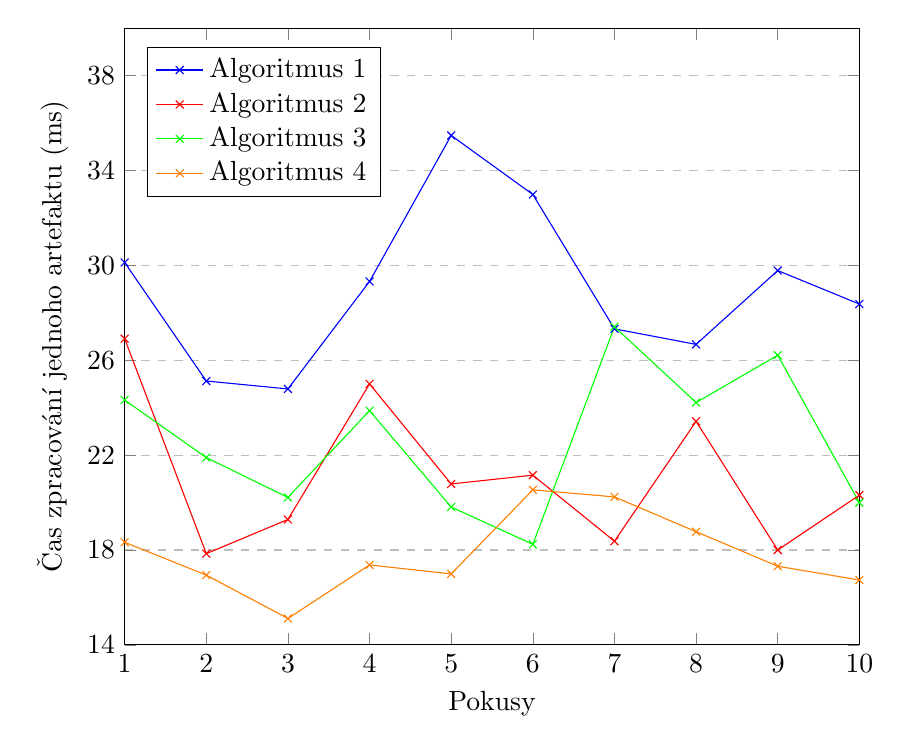
\begin{tikzpicture}
\pgfplotsset{%
    width=.9\textwidth,
}
\begin{axis}[
    title={},
    xlabel={Pokusy},
    ylabel={Čas zpracování jednoho artefaktu (ms)},
    xmin=1, xmax=10,
    ymin=14, ymax=40,
    xtick={1,2,3,4,5,6,7,8,9,10},
    ytick={10,14,18, 22, 26, 30, 34, 38},
    legend pos=north west,
    ymajorgrids=true,
    grid style=dashed,
]

\addplot[
    color=blue,
    mark=x,
    ]
    coordinates {(1,30.122)(2,25.124)(3,24.789)(4,29.323)(5,35.478)(6,32.989)(7,27.324)(8,26.668)(9,29.782)(10,28.369)};
  \addplot[
    color=red,
    mark=x,
    ]
    coordinates {
(1, 26.909)
(2, 17.845)
(3, 19.285)
(4, 25.002)
(5, 20.783)
(6, 21.154)
(7, 18.369)
(8, 23.423)
(9, 17.998)
(10, 20.312)
    };

    \addplot[
    color=green,
    mark=x,
    ]
    coordinates {
(1, 24.321)
(2, 21.897)
(3, 20.214)
(4, 23.875)
(5, 19.811)
(6, 18.237)
(7, 27.412)
(8, 24.217)
(9, 26.211)
(10, 19.996)
    };

    \addplot[
    color=orange,
    mark=x,
    ]
    coordinates {
(1, 18.324)
(2, 16.940)
(3, 15.111)
(4, 17.369)
(5, 16.989)
(6, 20.535)
(7, 20.237)
(8, 18.770)
(9, 17.315)
(10, 16.732)
    };

\legend{Algoritmus 1, Algoritmus 2, Algoritmus 3,  Algoritmus 4}
\end{axis}
\end{tikzpicture}
\caption{Časy přečtení a získání jednoho artefaktu z~XML souboru v~milisekundách}
\label{fig:xml_read_plot}
\end{figure}

\newpage

Z~výsledků analýzy můžeme vidět, že nejrychlejší algoritmus pro přečtení a zpracování jednoho artefaktu je algoritmus číslo 4, který používá pouze cykly a objekty \textit{SimpleXMLElement}. Druhý nejrychlejší byl na základě analýzy algoritmus 2, který kombinuje technologii XPath a objekty \textit{SimpleXMLElement}. Poté následují nejpomalejší algoritmy 3 a 1.

Výhodou nejrychlejšího algoritmu 4 je kromě rychlosti také možnost  používat metody pro přístup k~atributům daného objektu. Bohužel existuje zde velká nevýhoda spočívající ve formě složitosti a délce celého kódu, který je navíc kvůli velkého počtu cyklů pro vnořené elementy velmi nepřehledný. Zároveň dle dalších testů je velmi pravděpodobné, že se rychlost razantně zpomalí při čtení více artefaktů za sebou, jelikož se zaplní paměť velkým množstvím objektů \textit{SimpleXMLElement}.

Z~tohoto důvodu byl pro implementaci, extrakci a zpracování dat artefaktů z~XML zvolen algoritmus 2, který kombinuje technologii XPath a objekty typu \textit{SimpleXMLElement}. Pro základní iteraci a základní elementy je používán XPath. Tento způsob kromě dobré rychlosti zaručuje i to, že celý kód nebude tak složitý jako v~případě čtvrtého algoritmu.

Nejprve se jednotlivé elementy uloží do pole dle identifikátoru daného elementu. Zároveň se jejich jednotlivé atributy zařadí do vícerozměrného pole dle identifikátoru daného artefaktu. Jakmile je celý XML soubor pro daný projekt přečtený, veškeré artefakty se namapují na pole objektů typu \textit{RmArtifact}. Důvod, proč se elementy z~XML souboru nemapují rovnou na objekty \textit{RmArtifact}, spočívá v~automatizaci čtení XML souboru.

Dále jsou tyto soubory validovány a jejich data jsou upravována a transformována do požadované formy. Tyto objekty vzniklé stažením dat z~platformy IBM Jazz se poté mapují na dokumenty a ukládají do NoSQL MongoDB databáze. Při tomto procesu se kontroluje, zda daný artefakt již neexistuje a nemá se pouze vytvořit nová verze daného artefaktu dle data stažení. Pakliže daný artefakt neexistuje, artefakt se založí a vytvoří se první verze artefaktu.

\section{Zobrazení dat}
Jakmile jsou data z~platformy IBM Jazz stažena a naimportována, lze  si je zobrazit jak v~administraci, tak v~uživatelské části daného projektu. Data zobrazovaná v~administrátorské části jsou pouze textová. V~administrační části se nenachází žádné grafické zobrazení dat, jelikož administrační část slouží zejména pro správu celé aplikace a vytváření definic metrik. Textové zobrazení je vypisováno zejména v~tabulkách. Tento přístup byl zvolen zejména z~toho důvodu, že administrátor nepotřebuje vidět detailně daná data a také nepotřebuje přímo s~nimi pracovat.

Jak již bylo zmíněno, možnost zobrazení všech stahovaných dat se také nachází v~uživatelské sekci prototypového nástroje, která je přístupná pro všechny registrované uživatele. Jednotlivá stahovaná data se seskupují podle projektu a modulu, do něhož patří. Na výpisech je možno si data buď zobrazit pro všechny projekty a moduly nebo je také možno si data vyfiltrovat dle definovaného projektu či modulu. Data je možno zobrazit jak na výpisech jednotlivých typů dat, tak na detailním náhledu. Oproti administrační části celého systému je zde možnost si data, zejména pak metriky, zobrazit graficky pomocí grafu.

% předpříprava dat query language

\section{Definice a vytváření metrik}
Pokud si uživatel přeje vytvořit metriku úplně od základu včetně nové definice metriky, bude nejprve potřebovat vytvořit definici dané metriky. Definice metriky může aktuálně vytvořit pouze administrátor v~administraci prototypového nástroje. Tento způsob byl zvolen z~toho důvodu, že administrátor vytvoří jednotlivé definice dle používaného standardu, nebo dle potřeb měření procesů daného projektu a společnosti, a až poté si uživatelé vytvářejí metriky. Veškeré definice se ukládají do NoSQL databáze pro snadnou a přehlednou manipulací s~celými objekty.

Administrátor vytváří definice metrik pomocí vícekrokového formuláře. V~prvním kroku vytvoření definice metriky se nachází základní údaje o~definici, jako je například název, popis nebo zda je daná metrika podílová či nikoli. Dále se v~druhém kroku formuláře nacházejí dynamická pole pro definování jednotlivých podmínek, dle kterých se bude řídit zobrazení konečné metriky. Jestliže uživatel zvolí, aby byla definice metriky podílová, může zvolit podmínky pro druhé měření, které bude první podmínky dělit. Podmínky je možno volit pomocí polí, v~nichž lze vyhledávat. Třetí krok slouží pro kontrolu vygenerovaných podmínek, které z~formuláře vzniknou. Celá definice metriky je nezávislá na modulech a projektu. Tyto údaje se poté volí až při vytváření samotné metriky. Daný způsob byl zvolen jednak pro možnost využití různých definic pro více druhů metrik, jednak i na doporučení vedoucího práce Ing. Svatopluka Štolfy, PhD. Celý proces vytváření definice metriky byl inspirován nástrojem \textit{Report builder}, který se nachází na platformě IBM Jazz. Druhý krok procesu vytváření definice metriky je možno vidět na obrázku \ref{fig:report_builder_admin}.

\begin{figure}[!ht]
    \centering
    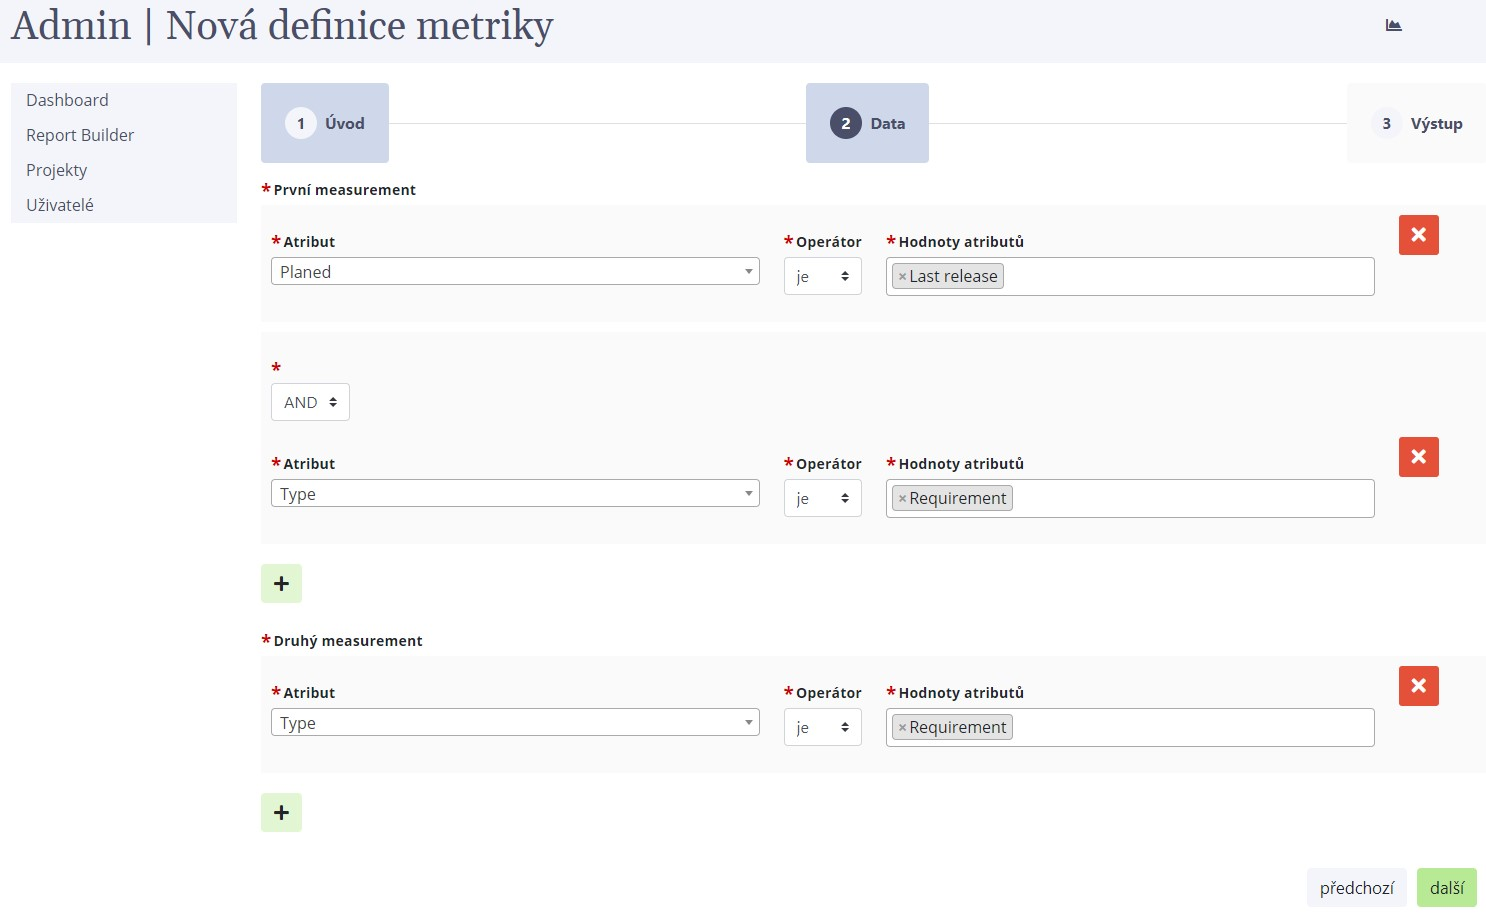
\includegraphics[width=1\textwidth]{Diplomka/Figures/report_builder.jpg}
    \caption{Proces vytváření definice metriky}
    \label{fig:report_builder_admin}
\end{figure}

Jakmile administrátor nebo skript vytvoří definice metrik dle používaného standardu, je možno vytvářet jednotlivé metriky. Metriky mohou vytvářet uživatelé v~uživatelské části ve formuláři, který je vidět na obrázku \ref{fig:new_metric_from}. Při vytváření metriky je nutno zvolit například název, definicí, pomocí které má metrika agregovat data, z~jakého projektu a případně z~jakých modulů má metrika data čerpat. Jedna metrika musí mít vždy zvolený projekt, k~němuž patří. Dále je například možno zvolit typ grafu, jakým budou data v~rámci metriky vizualizována. Jednotlivé metriky je možno poté filtrovat dle projektu, k~němuž patří. Povinnost vyplnění polí ve formuláři je, stejně jako v~celém nástroji, zobrazena pomocí červené hvězdičky.


\begin{figure}[!ht]
    \centering
    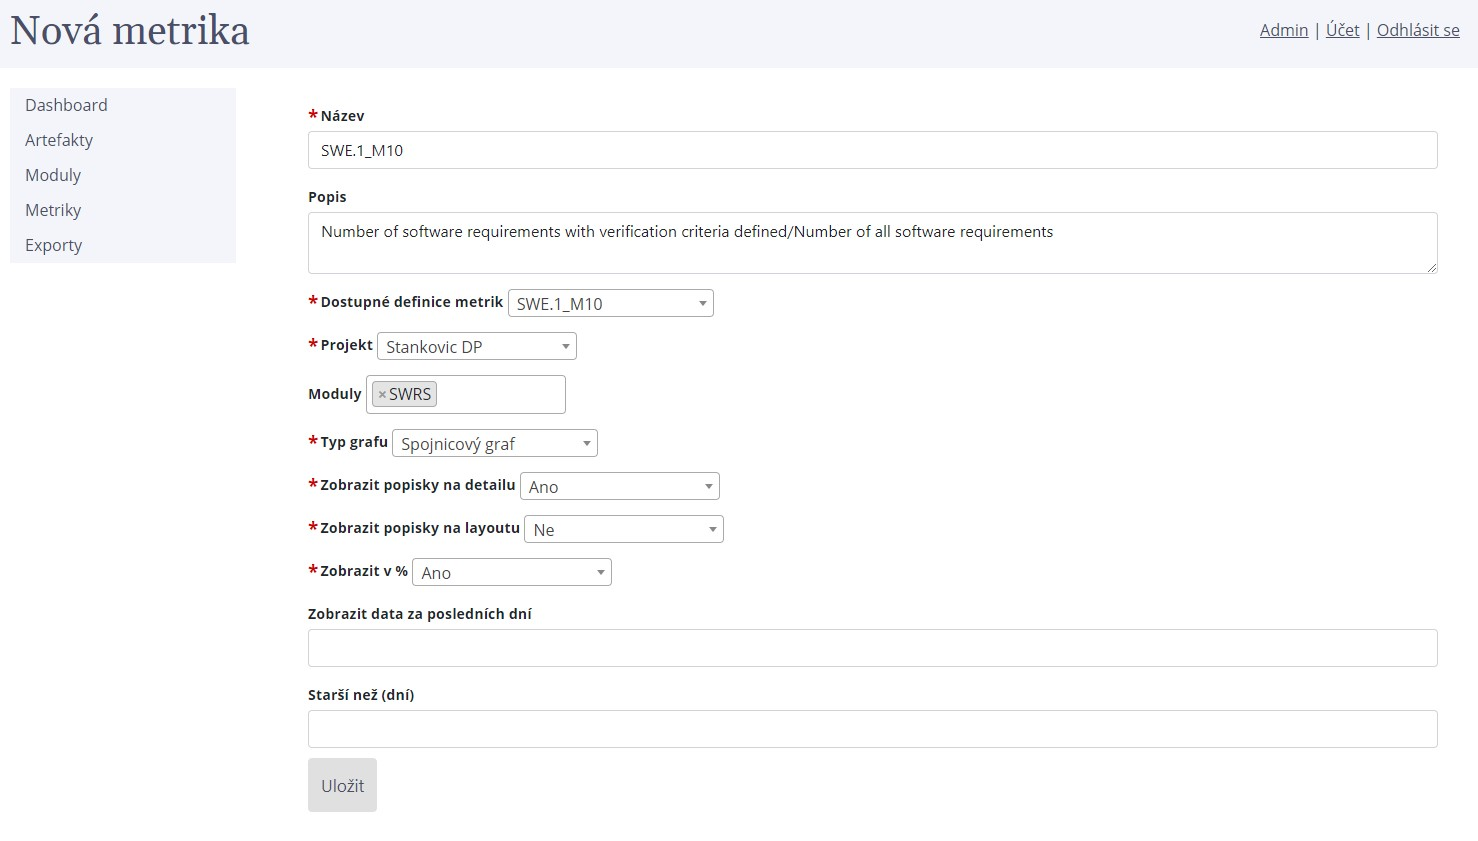
\includegraphics[width=1\textwidth]{Diplomka/Figures/new_metric_form.jpg}
    \caption{Formulář pro vytvoření metriky}
    \label{fig:new_metric_from}
\end{figure}

U~metriky můžeme také například zvolit, zda se mají na nástěnce nebo na detailu dané metriky zobrazovat v~grafu popisky. Tato funkcionalita byla po konzultaci zavedena zejména z~důvodu větší možnosti konfigurace a personalizace. Jelikož je v~rámci standardu Automotive SPICE nutno měřit data za určitý časový úsek, existuje v~nastavení metriky možnost nastavení takového omezení.

V~rámci praktické práce byly vytvořeny některé demonstrativní metriky na základě standardu Automotive SPICE. \cite{ref:metrics_and_dashboard_for_level_two} Demonstrativní data jsou řešena pomocí Symfony komponenty \textit{DataFixtures}, kterou je možno spustit a data do aplikace vložit pomocí příkazu \textit{composer db-demo} v~příkazovém řádku.

\section{Nástěnka}
V~uživatelské sekci se po přihlášení uživatele zobrazí stránka, kterou si může každý uživatel upravovat dle svých potřeb. Každý uživatel si na nástěnku může libovolně přidávat metriky pomocí výběru v~horní části stránky. Samozřejmostí je také možnost si zobrazené metriky z~nástěnky odstranit. Uživatelé si mohou dle libosti jednotlivé metriky na nástěnce řadit a přesouvat. Přesouvání funguje pomocí technologie JavaScript. Ukládaní a změna pořadí metriky jsou prováděny technologií AJAX na pozadí. Ukládání nástěnky tedy proběhne při jakékoli změně jejího rozvržení na pozadí bez nutnosti načíst znovu stránku. Pomocí této technologie funguje také odstraňování metrik z~nástěnky.

Nástěnka slouží zejména pro rychlou kontrolu metrik. Grafy metrik nelze totiž na nástěnce filtrovat, ani nijak podrobně zobrazovat. Typickým případem užití je, když manažer potřebuje získat rychlé informace o~průběhu projektu z~vícero metrik v~jednu chvíli. Dokáže například zjistit, zda se vývoj projektu ubírá správným směrem či nikoli. Z~nástěnky je možno po kliknutí na název metriky přesměrování na detailní výpis dané metriky. Dále je zde možnost si pomocí ikony třech teček metriku exportovat nebo nastavit. Nástěnku s~několika metrikami můžeme vidět na obrázku \ref{fig:dashboard_metrics}.

\begin{figure}[!ht]
    \centering
    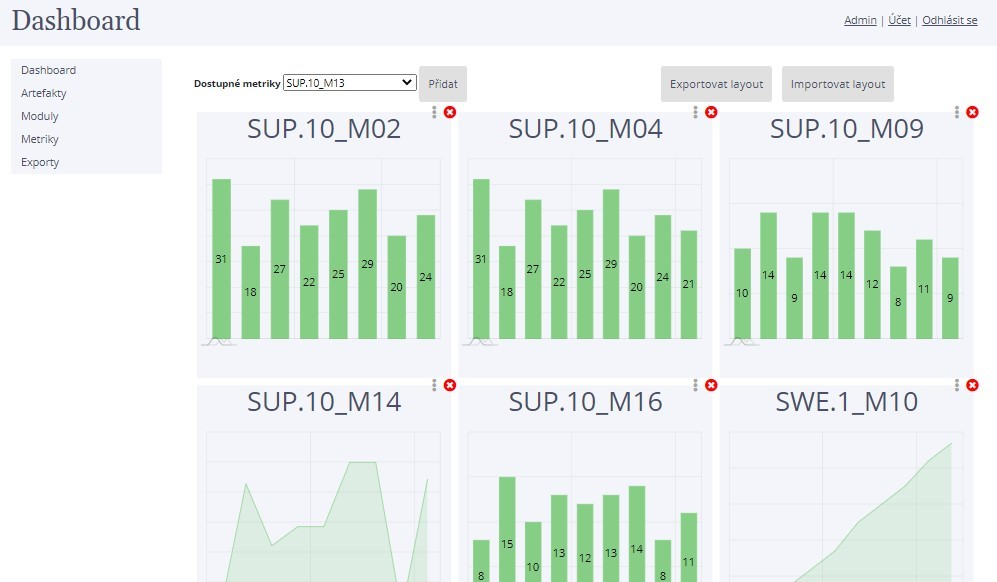
\includegraphics[width=1\textwidth]{Diplomka/Figures/dashboard_metrics.jpg}
    \caption{Nástěnka na úvodní obrazovce}
    \label{fig:dashboard_metrics}
\end{figure}

Celou individuální nástěnku si může každý uživatel exportovat nebo poté importovat například nástěnku jiného uživatele. Export nástěnky funguje na principu stažení XML souboru s~jednotlivými metrikami a pozicemi. Tento soubor je poté možno sdílet dalším uživatelům a následně naimportovat. Rovněž je možno tento soubor použít pro vlastní zálohu nástěnky a kdykoli si obnovit celou nástěnku do původního stavu. Nástěnka se pak zobrazí dle nahraného XML souboru.


\section{Zobrazení metrik}
Metriky je možno v~rámci nástroje zobrazit jak textově pomocí tabulky, tak i graficky podle zvoleného typu grafu v~nastavení metriky. Textové zobrazení je dostupné pouze na detailním zobrazení metriky v~uživatelské části nástroje. Vypočítaná data metriky v~tabulce jsou seskupena dle data sběrů, tedy kdy byly dané artefakty naimportovány z~platformy IBM Jazz. V~tabulce se již vyskytují agregovaná data, která mohou být zobrazena podle nastavení metriky buď v~procentech, nebo jako prosté číslo.

Na detailním výpisu je dále zobrazen graf dle zvoleného typu grafu. V~teoretické části této práce byly zvoleny pro analýzu určité JavaScript knihovny, které je možno nalézt v~kapitole \ref{sec:visualisation}. První z~knihoven pro zobrazení grafů byla analyzována knihovna Google Charts. Mezi výhody, které nabízí, patří možnost plného použití zdarma a velké množství typů grafů. Během analýzy však bylo zjištěno, že grafy nejsou interaktivní a není možno bez obnovení stránky graf filtrovat a upravovat.

Mezi další možnou knihovnu patří knihovna amCharts, která generuje grafy pomocí SVG obrázků. Jejími výhodami jsou velké množství grafů, možnost použít různé animace pro zobrazení či interaktivnost všech grafů. V~grafu je možno bez nutnosti obnovení stránky filtrovat nebo omezovat vykreslení dle data. Mezi nevýhody může patřit placená licence v~případě potřeby zobrazit graf bez malého loga v~rohu.

Poslední analyzovaná knihovna byla Chart.js, která je oproti předchozím knihovnám velmi malá a jednoduchá. Nabízí pouze pár grafů, které mohou být interaktivní stejně jako v~případě knihovny amCharts. Nevýhodou této knihovny je až přílišná jednoduchost a s~tím spojená omezenost pro vykreslování složitějších dat.

Pro zobrazení grafu na základě analýzy byla zvolena knihovna \textit{amCharts} jelikož poskytuje velké množství konfigurací a filtrování bez nutnosti opětovného načtení stránky. Mezi další výhody patří mnoho existujících návodů na nasazení grafů do webové stránky. Implementace knihovny do nástroje je provedena pomocí JavaScriptu. V~rámci skriptu probíhá veškeré nastavení grafu a vkládání dat do grafu pomocí formátu JSON. Na stejném principu funguje i zobrazení grafů na nástěnce, kdy pro každý graf je vygenerován skript s~daty a vypsán do HTML stránky. Výsledné zobrazení spojnicového grafu a tabulky v~rámci metriky je možno vidět na obrázku \ref{fig:metric_detail}.

\begin{figure}[!ht]
    \centering
    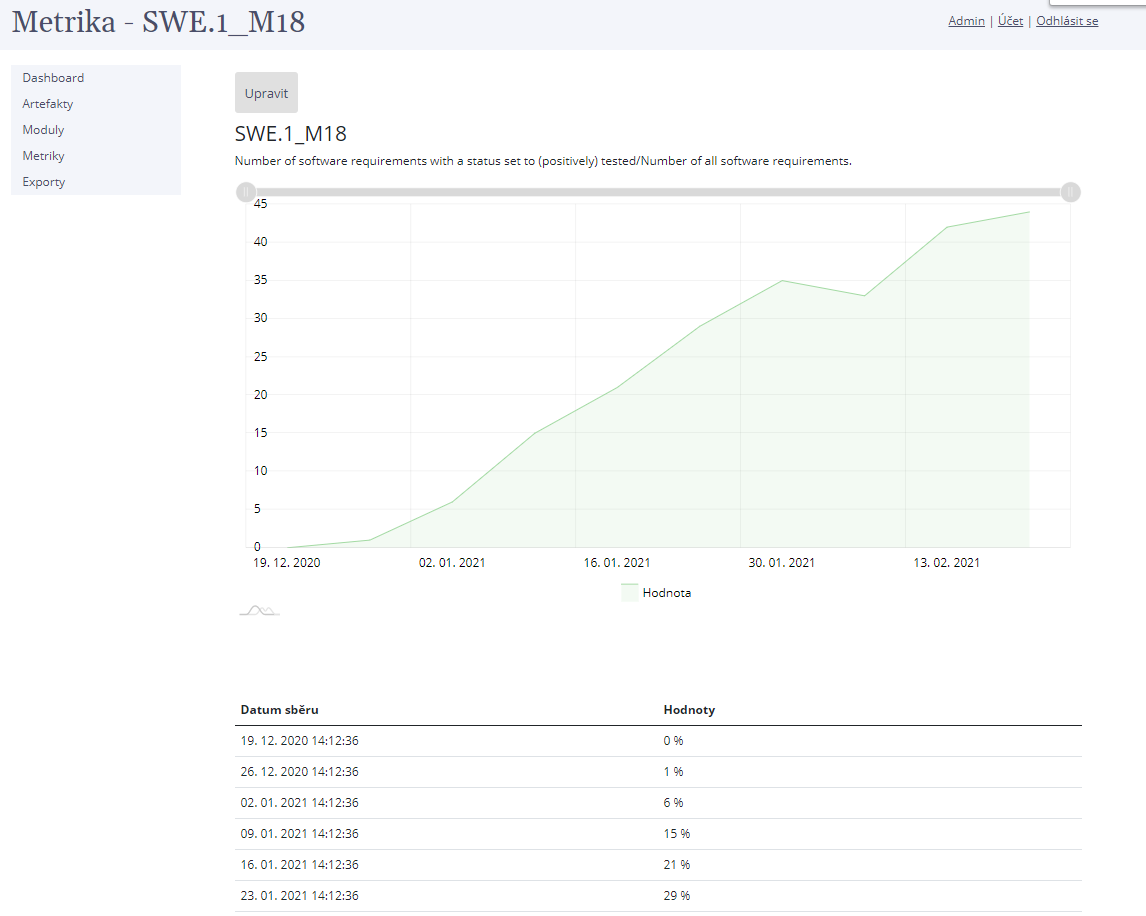
\includegraphics[width=1\textwidth]{Diplomka/Figures/metric_detail.png}
    \caption{Detailní výpis metriky}
    \label{fig:metric_detail}
\end{figure}


\section{Výstupní reporty a exporty metrik}
\label{sec:reports}
Kromě zobrazení metrik pomocí tabulky a grafu ve webové aplikaci je vhodné mít tyto výsledky i v~podobě, v~níž není potřeba pro zobrazení internet. Tato možnost je rovněž vhodná pro prezentování výsledků vývoje. Díky tomu může například manažer vyššímu vedení pomocí metrik zobrazených v~prezentaci nebo dokumentu prezentovat, jak daný projekt postupuje či jak je jeho tým efektivní. Právě kvůli těmto případům užití byly v~rámci nástroje vyvinuty exporty metrik.

V~rámci nástroje byly vyvinuty dva typy exportu metrik. První možností exportu je exportování samostatné metriky. Tento export slouží pro pouhé stažení dat, případně grafu metriky. Pomocí exportu si lze metriku stáhnout do několika formátů, mezi něž patří Microsoft Word a PowerPoint. Dále je možno stáhnout agregovaná data ve formátu CSV. Data jsou poté stažena ve formátu se dvěma sloupci -- datum sběru a hodnota. Vyvolat daný export je možno buď přímo z~nástěnky u~metriky, kterou chce uživatel stáhnout, nebo na výpise jednotlivých metrik či na detailním zobrazení dané metriky. Tlačítko pro export je možno vidět na obrázku \ref{fig:dashboard_export}.

\begin{figure}[!ht]
    \centering
    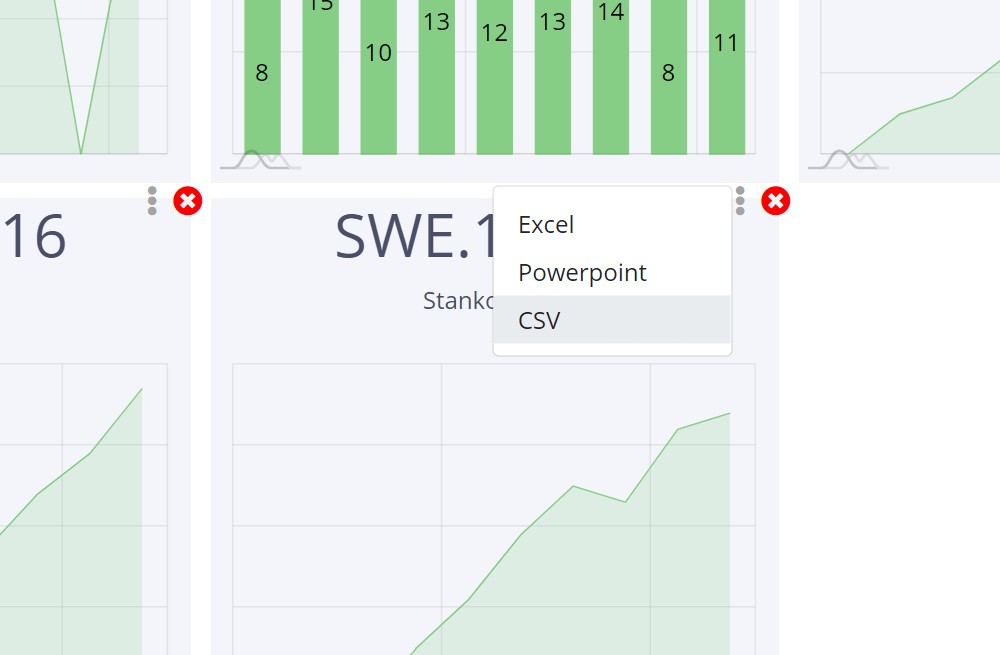
\includegraphics[width=0.8\textwidth]{Diplomka/Figures/dashboard_export.jpg}
    \caption{Export metriky z~nástěnky}
    \label{fig:dashboard_export}
\end{figure}

Druhou možností exportu dat je export pomocí takzvaných dokumentů. Tento způsob je možno také nalézt například v~nástroji codeBeamer ALM nebo Siemens Polarion, které jsou popsány v~kapitole \ref{sec:alm}. Hlavní předností tohoto exportu je možnost vytvořit si dokument, do kterého je vloženo několik metrik jak ve formě grafického zobrazení, tak pomocí tabulkového zobrazení. Mezi tyto metriky je možno vložit libovolné množství odstavců textu a jejich nadpisů. Díky tomu může uživatel vytvořit dokument, do něhož vloží jednotlivé sekce dle potřeby. Dokument je vhodný například pro již zmíněnou prezentaci výsledků daného vývojového týmu. Dokumenty se ukládají do MongoDB databáze, přičemž jednotlivé sekce dokumentu jsou uloženy jako vložené objekty do hlavního objektu celého dokumentu.

Dokumenty můžeme vytvořit na stránce nazvané \textit{Dokumenty}. Stránka se nachází na uživatelské straně nástroje. Při vytvoření dokumentu si uživatel zvolí název, popis, projekt a formát exportu. Poté si může přidávat  jednotlivé bloky s~textem, grafem nebo tabulkou metriky. Takto si může pohodlně a dynamicky vytvořit celý dokument. Ten je poté možno pomocí tlačítka exportovat do vybraného formátu, mezi které patří Microsoft Word a PowerPoint. Přičemž je možné v budoucnu tyto exporty jednoduše rozšířit o~formáty PDF a~HTML. Pokaždé, když si uživatel dokument otevře nebo exportuje, vidí aktuální stav jednotlivých metrik. Celý dokument je tedy živá stránka, která se aktualizuje dle nejnovějších dat. Proces vytváření dokumentu je možno vidět na obrázku \ref{fig:report_document}. Detailní výpis ve webovém nástroji vygenerovaného dokumentu můžeme vidět na obrázku \ref{fig:report_document_detail}.

\begin{figure}[!ht]
    \centering
    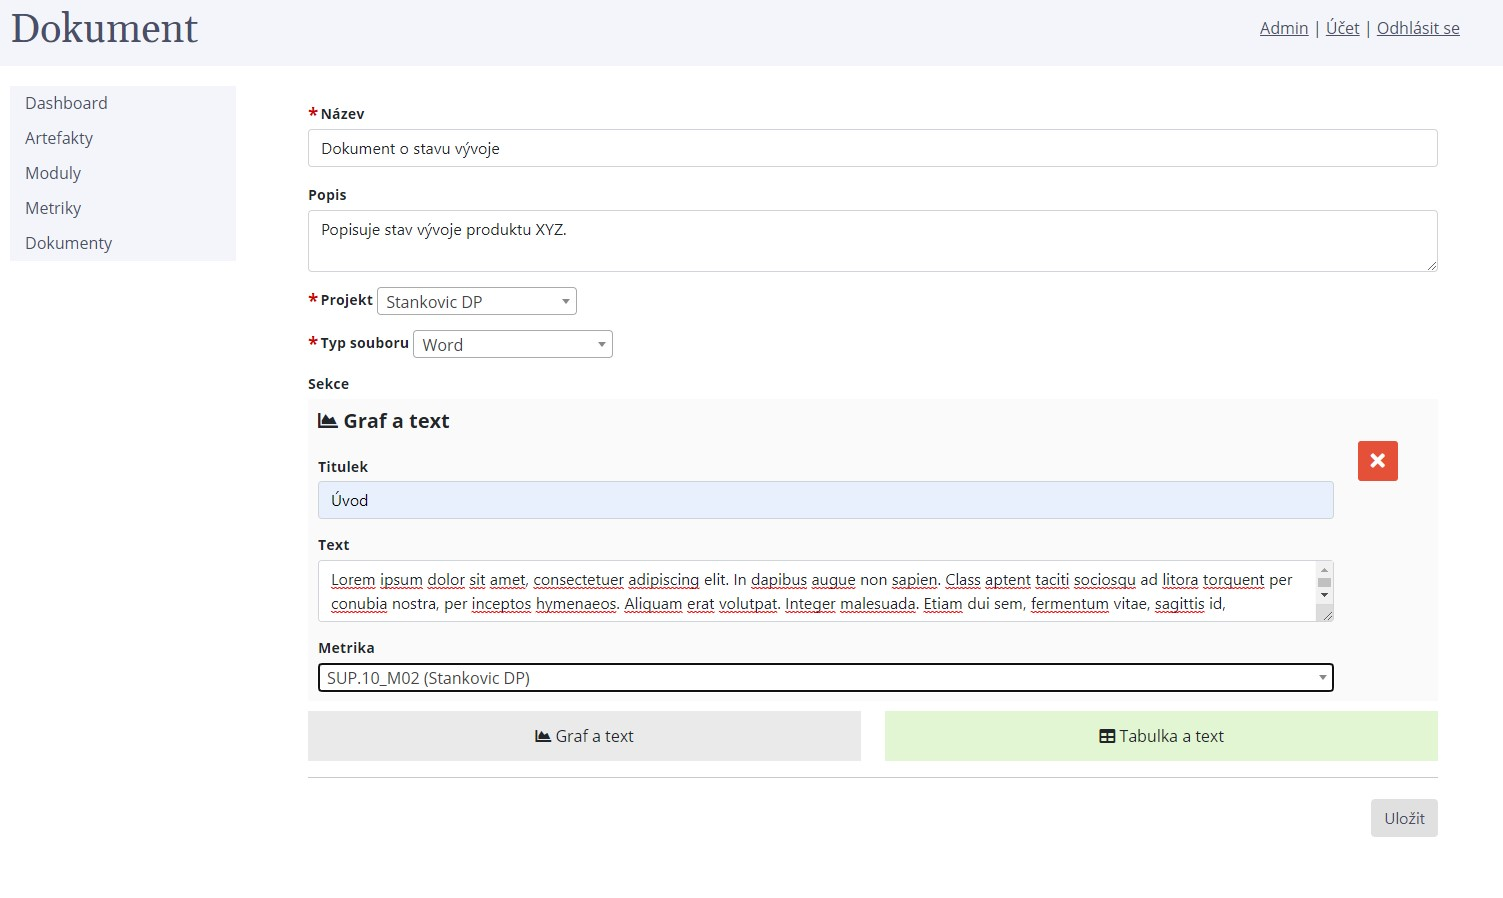
\includegraphics[width=0.9\textwidth]{Diplomka/Figures/report_document.jpg}
    \caption{Proces vytváření dokumentu}
    \label{fig:report_document}
\end{figure}

\begin{figure}[!ht]
    \centering
    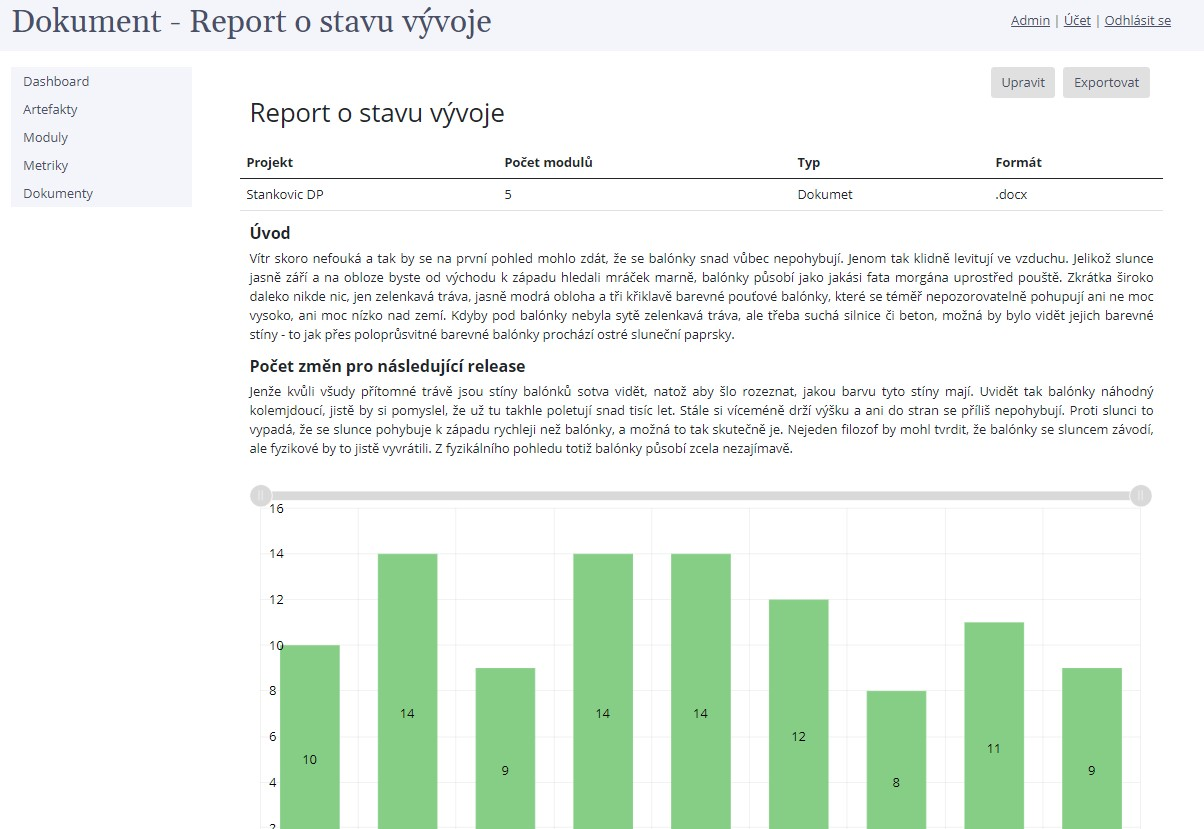
\includegraphics[width=0.9\textwidth]{Diplomka/Figures/report_document_detail.jpg}
    \caption{Detailní výpis vygenerovaného dokumentu v~nástroji}
    \label{fig:report_document_detail}
\end{figure}

Veškeré exporty do formátů pro programy Microsoft Office jsou naprogramovány pomocí knihovny \textit{PhpOffice}, která je volně dostupná na platformě \textit{GitHub} \cite{ref:phpoffice}. V~rámci knihovny se používají moduly \textit{PhpSpreadsheet} pro export do formátu Excel, \textit{PhpPresentation}pro export dat do formátu PowerPoint a \textit{PHPWord} pro exportování do formátu Word. Pro exportování do ostatních formátů, mezi něž patří například CSV, je použito klasických knihoven jazyka PHP.


\chapter{Závěr}
Clem práce bylo kromě vytvoření prototypového nástroje pro sledování a zobrazení metrik potřebných pro splnění standardu Automotive SPICE také analyzovat a prozkoumat již existující nástroje pro správu životního cyklu vývoje celého produktu, měření kvalit softwarových procesů, sběru artefaktů a nakonec i samotná správa softwarových procesů.

Teoretická část této práce je věnována studiu obecné oblasti softwarového inženýrství, softwarovým procesům, správě životního cyklu aplikace, sběru artefaktů a také standardu Automotive SPICE. V~rámci teoretické části byly rozebrány jednotlivé části softwarového procesu -- plánování, monitorování a uzpůsobení, které jsou důležité pro pochopení vyvíjeného prototypového nástroje v~praktické části této práce. Dodržování určitého standardu přináší výhody ve formě efektivnějšího vývoje, lepší správy procesů, ale také lepší kontrolu kvality výsledného produktu. Aby bylo možno hodnotit kvalitu celého projektu, je nutno procesy a jejich výsledky hodnotit. Hodnocení je vhodné vizualizovat v~čase, přičemž jednou z~možností je využití metriky. Za pomocí metrik dokážeme hodnotit výsledky procesu a zajistit správné směřování celého projektu.

Hlavním praktickým cílem této práce bylo vytvoření nástroje pro sledování a zobrazení metrik. Vytvoření tohoto prototypového nástroje neprobíhalo pouhou implementací a programováním.  Během práce na praktické části jsem si vyzkoušel v~praxi vývoj nástroje pomocí celého vývojového cyklu.Jednou z~nejdůležitějších a počátečních fází byla analýza a sběr požadavků, jež byly na výsledný nástroj kladeny. Během analýzy byly vytvářeny jednak případy užití, ale také celkový návrh architektury a uživatelského rozhraní nástroje. Během samotného vytváření nástroje probíhaly s~vedoucím práce konzultace na bázi čtrnáctidenních iterací, při nichž byly stanoveny priority, které se budou vždy následující dny řešit.

Jednou z~důležitých fází návrhu a implementace nástroje bylo napojení na platformu IBM Jazz. Pro implementaci napojení bylo po zevrubné analýze vybráno řešení spočívající v~napojení pomocí REST API, které nabízí možnost automatizovaného stahování dat z~této platformy. Tento přístup byl namísto OSLC zvolen zejména díky možnosti stahovat uživatelské atributy artefaktů včetně propojení s~jinými artefakty. Tuto funkcionalitu bohužel OSLC v~době vypracovávání práce nenabízelo. Takto stahované artefakty jsou ukládány do NoSQL databáze, která nabízí možnost ukládat složité objekty. Velkou výhodou oproti ostatním existujícím podobným nástrojům je možnost stahované artefakty verzovat a ukládat dle data stažení. Díky tomu může uživatel nástroje vidět, jak se jednotlivé artefakty mění v~čase.

Díky ukládání artefaktů v~čase je následně možno vytvářet a definovat trendové metriky, které jsou důležité pro splnění standardu Automotive SPICE. U~artefaktů jsou z~platformy IBM Jazz ukládány veškeré atributy včetně uživatelských. Administrátor může nejen dle specifikací tohoto standardu vytvořit definice metriky. Během definice metriky lze vytvořit podmínky ze všech možných atributů, které byly v~nástroji v~minulosti staženy a naimportovány z~platformy IBM Jazz. Dále je možno u~definice metriky nastavit, z~jakých modulů má výsledná metrika čerpat data. Definice metrik nejsou závislé na projektu a jsou tedy jednoduše znovupoužitelné na jiném projektu. Z~těchto definic poté uživatelé vytvářejí samotné metriky vázané na určitý projekt, které lze zobrazit pomocí tabulky a vizualizovat pomocí grafu. Metriky lze třídit dle projektu a zobrazit buď na nástěnce, která je konfigurovatelná pro každého uživatele, nebo na detailním výpisu určité metriky. Veškeré tyto funkcionality vychází jak z~existujících nástrojů, tak právě naopak z~funkčností, které v~těchto nástrojích chybí a jsou důležité pro splnění standardu Automotive SPICE. Vygenerované metriky v~čase lze exportovat například do formátů pro programy Microsoft Office, CSV, nebo PDF. Exportování je možné pomocí dokumentů, kdy si uživatel může k~exportu kromě tabulek a grafů doplnit také text a nadpisy jako v~běžném dokumentu. Nástroj nabízí také exportování jednotlivých metrik samostatně. Samozřejmostí prototypového nástroje je nutnost přihlášení a správa uživatelů, které lze rozdělit na administrátory a běžné uživatele.

Vyvinutý nástroj je univerzální a lze jej použít prakticky na jakékoli sledování určitého procesu nebo samotného vývoje. Do prototypového nástroje je možno kdykoli pomocí jednoho příkazu nahrát ukázková data. Ukázková data obsahují kromě náhodně vygenerovaných artefaktů také metriky vycházející z~požadavků na splnění standardu Automotive SPICE. Nástroj je vytvořen jako podniková webová aplikace, která je nezávislá na platformě a pro práci v~ní je potřeba běžný webový prohlížeč.

Během celé práce na vývoji prototypového nástroje jsem se zdokonalil nejen ve vývoji podnikové webové aplikace, ale mohl jsem si také v~praxi vyzkoušet celý vývojový proces od analýzy až po implementaci a testování pomocí nejen automatických testů. Výsledný nástroj je postaven na moderních technologiích a je snadno rozšiřitelný o~další možné funkcionality. Během celé implementace byla kromě automatického testování použita kontrola a oprava standardů zdrojového kódu. Výsledný zdrojový kód je psán s~ohledem na nejmodernější principy dle platných standardů. Z~mého osobního hlediska má pro mě práce velký přínos a pevně věřím, že vyvinutý nástroj najde uplatnění v~praxi či bude rozšířen v~budoucnu o~nové funkcionality.

\begin{thebibliography}{43}

\bibitem{ref:sommerrville_sw_process}
SOMMERVILLE, Ian. \textit{Software engineering}. 9th edition. Boston: Addison-Wesley, 2011, s.~28-29. ISBN 978-0-13-703515-1.

\bibitem{ref:sw_process_vondrak}
\textit{Úvod do softwarového inženýrství} [online]. In: VONDRÁK, Ivo. Ostrava, 2002, s. 3 [cit. 2020-11-30]. Dostupné z: http://vondrak.cs.vsb.cz/download/Uvod\_do\_softwaroveho\_inzenyrstvi.pdf

\bibitem{ref:cmm_cmmi}
Software measurement and metrics. SOMMERVILLE, Ian. \textit{Software engineering}. 9th edition. Boston: Addison-Wesley, 2011, s.~721-722. ISBN 978-0-13-703515-1.

\bibitem{ref:sommerrville_waterfall}
SOMMERVILLE, Ian. \textit{Software engineering}. 9th edition. Boston: Addison-Wesley, 2011, s.~29-32. ISBN 978-0-13-703515-1.

\bibitem{ref:rup_ibm_about}
\textit{Rational Unified Process: Best Practices for Software Development Teams} [online]. In: . Rev 11/01. Cupertino: Rational Software, 1998, s.~1 [cit. 2020-11-21]. Dostupné z: https://www.ibm.com/developerworks/rational/library/content/03July/
1000/1251/1251\_bestpractices\_TP026B.pdf

\bibitem{ref:rup_ibm}
\textit{Rational Unified Process: Best Practices for Software Development Teams} [online]. In: . Rev 11/01. Cupertino: Rational Software, 1998, s.~3 [cit. 2020-11-21]. Dostupné z: https://www.ibm.com/developerworks/rational/library/content/03July/
1000/1251/1251\_bestpractices\_TP026B.pdf

\bibitem{ref:agilne_manifesto}
\textit{Manifest Agilního vývoje software} [online]. 2001 [cit. 2020-11-21]. Dostupné z: https://agilemanifesto.org/iso/cs/manifesto.html

\bibitem{ref:sommerrville_agile_products}
SOMMERVILLE, Ian. \textit{Software engineering}. 9th edition. Boston: Addison-Wesley, 2011, s.~59. ISBN 978-0-13-703515-1.

\bibitem{ref:what_is_xp}
BECK, Kent a Cynthia ANDRES. \textit{Extrémní programování: embrace change}. 2nd ed. Praha: Grada, 2002, s.~1---7. Moderní programování. ISBN 80-247-0300-9.

\bibitem{ref:scrum_myslin}
MYSLÍN, Josef. \textit{Scrum: průvodce agilním vývojem softwaru}. Brno: Computer Press, 2016. ISBN 978-80-251-4650-7.

\bibitem{ref:scrum_myslin_cyklus_img}
MYSLÍN, Josef. \textit{Scrum: průvodce agilním vývojem softwaru}. Brno: Computer Press, 2016 s.~85. ISBN 978-80-251-4650-7.

\bibitem{ref:scrum_myslin_us}
MYSLÍN, Josef. \textit{Scrum: průvodce agilním vývojem softwaru}. Brno: Computer Press, 2016 s.~89. ISBN 978-80-251-4650-7.

\bibitem{ref:vmodel_Tierno2016}
TIERNO, Antonio, Max M. SANTOS, Benedito A. ARRUDA a Joao N. H. DA ROSA. Open issues for the automotive software testing. \textit{2016 12th IEEE International Conference on Industry Applications (INDUSCON)} [online]. IEEE, 2016, 2016, , 1-8 [cit. 2020-11-27]. ISBN 978-1-5090-5127-4. Dostupné z: doi:10.1109/INDUSCON.2016.7874609

\bibitem{ref:metric_definition}
Software measurement and metrics. SOMMERVILLE, Ian. \textit{Software engineering}. 9th edition. Boston: Addison-Wesley, 2011, s.~668. ISBN 978-0-13-703515-1.


\bibitem{ref:kontrolni_metriky}
Software measurement and metrics. SOMMERVILLE, Ian. \textit{Software engineering}. 9th edition. Boston: Addison-Wesley, 2011, s.~711-7114. ISBN 978-0-13-703515-1.

\bibitem{ref:birt_about}
BIRT Design Overview. \textit{BIRT} [online]. Ottawa: The Eclipse Foundation, 2014, 2014 [cit. 2020-11-28]. Dostupné z: https://www.eclipse.org/birt/about/

\bibitem{ref:metabase}
\textit{Metabase} [online]. San Francisco: Metabase, c2021 [cit. 2021-01-15]. Dostupné z: https://www.metabase.com/

\bibitem{ref:google_charts}
Charts | Google Developers. \textit{Google} [online]. [cit. 2021-01-08]. Dostupné z: https://developers.google.com/chart

\bibitem{ref:amcharts_web}
\textit{JavaScript Charts \& Maps - amCharts} [online]. amCharts, c2006-2021 [cit. 2021-01-15]. Dostupné z: https://www.amcharts.com/

\bibitem{ref:chartjs}
\textit{Chart.js | Open source HTML5 Charts for your website} [online]. https://www.chartjs.org/, c2021 [cit. 2021-01-15]. Dostupné z: https://www.chartjs.org/

\bibitem{ref:aspice_download_obecne}
Automotive SPICE | Download. \textit{Automotive SPICE} [online]. 2005, 2018 [cit. 2020-11-17]. Dostupné z: http://www.automotivespice.com/download/

\bibitem{ref:aspice_download_verze}
\textit{Automotive SPICE Process Reference and Assessment Model - Release 3.1} [online]. \textbf{1 November 2017}, s.~4 [cit. 2020-11-17]. Dostupné z: http://www.automotivespice.com/download/

\bibitem{ref:aspice_download_procesni_modely}
\textit{Automotive SPICE Process Reference and Assessment Model - Release 3.1} [online]. \textbf{1 November 2017}, s.~8 [cit. 2020-11-17]. Dostupné z: http://www.automotivespice.com/download/

\bibitem{ref:aspice_download_prm}
\textit{Automotive SPICE Process Reference and Assessment Model - Release 3.1} [online]. \textbf{1 November 2017}, s.~12-15 [cit. 2020-11-17]. Dostupné z: http://www.automotivespice.com/download/


\bibitem{ref:aspice_procesy}
\textit{Automotive SPICE Process Reference and Assessment Model - Release 3.1} [online]. \textbf{1 November 2017}, s.~13-15 [cit. 2021-01-01]. Dostupné z: http://www.automotivespice.com/download/

\bibitem{ref:aspice_download_1523}
\textit{Automotive SPICE Process Reference and Assessment Model - Release 3.1} [online]. \textbf{1 November 2017}, s.~15-23 [cit. 2020-11-18]. Dostupné z: http://www.automotivespice.com/download/

\bibitem{alm_chappell}
\textit{What is Application Lifecycle Management?} [online]. 2014, , 2-4 [cit. 2020-11-15]. Dostupné z: http://davidchappell.com/writing/white\_papers/What-is-ALM--Chappell.pdf

\bibitem{ref:about_codebeamer}
CodeBeamer ALM: Application Lifecycle Management Software. \textit{CodeBeamer ALM \& Intland Retina }[online]. Stuttgart: Intland Software, c1998-2021 [cit. 2021-01-20]. Dostupné z: https://intland.com/codebeamer/application-lifecycle-management/

\bibitem{ref:codebeamer_templates}
Templates. \textit{CodeBeamer ALM \& Intland Retina} [online]. Stuttgart: Intland Software, c1998-2021 [cit. 2021-01-20]. Dostupné z: https://intland.com/intland-templates/

\bibitem{ref:codebeamer_pricing}
CodeBeamer Subscription Pricing \& Features. \textit{CodeBeamer ALM \& Intland Retina} [online]. Stuttgart: Intland Software, c1998-2021 [cit. 2021-01-21]. Dostupné z: https://intland.com/codebeamer/pricing/

\bibitem{ref:codebeamer_rest}
REST API. \textit{CodeBeamer ALM \& Intland Retina} [online]. Stuttgart: Intland Software, c1998-2021 [cit. 2021-01-22]. Dostupné z: https://codebeamer.com/cb/wiki/117612

\bibitem{ref:polarion_about}
Polarion ALM. \textit{Siemens} [online]. Munich: Siemens Industry Software, c2020 [cit. 2021-01-23]. Dostupné z: https://polarion.plm.automation.siemens.com/products/polarion-alm

\bibitem{ref:polarion_extensions}
Polarion Extension Portal. \textit{Polarion Extensions} [online]. Munich: Siemens Industry Software, c2020 [cit. 2021-01-23]. Dostupné z: https://extensions.polarion.com/

\bibitem{ref:polarion_documentation}
Polarion ALM Software Development Kit. \textit{Siemens Polarion} [online]. Munich: Polarion, c2020 [cit. 2021-01-23]. Dostupné z: https://almdemo.polarion.com/polarion/sdk/index.html

\bibitem{ref:jazz}
\textit{Jazz Comunity Site} [online]. IBM, c2021 [cit. 2021-01-24]. Dostupné z: https://jazz.net/

\bibitem{ref:jazz_products}
IBM Jazz Products. Jazz Comunity Site [online]. IBM, c2021 [cit. 2021-01-24]. Dostupné z: https://jazz.net/products

\bibitem{ref:ibm_jazz_erm_dn}
IBM Engineering Requirements Management DOORS Next. \textit{IBM} [online]. IBM, c2021 [cit. 2021-01-24]. Dostupné z: https://www.ibm.com/products/requirements-management-doors-next

\bibitem{ref:bi_loshin_david}
LOSHIN, David. \textit{Business Intelligence: The Savvy Manager's Guide}. San Francisco: Morgan Kaufmann, 2003, 1 - 9. ISBN 978-1-55860-916-7.

\bibitem{ref:qlik_general}
Qlik Sense | Data Analytics Platform: Agent of transformation. Qlik [online]. King of Prussia: Qlik Technologies, c1993-2021 [cit. 2021-01-30]. Dostupné z: https://www.qlik.com/us/products/qlik-sense

\bibitem{ref:microsoft_bi_general}
Vizualizace dat | Microsoft Power BI. \textit{Microsoft Power BI} [online]. Redmond: Microsoft, c2021 [cit. 2021-01-27]. Dostupné z: https://powerbi.microsoft.com/cs-cz/

\bibitem{ref:php_trend}
Historical trends in the usage statistics of server-side programming languages for websites. \textit{W3Techs} [online]. Maria Enzersdorf: Q-Success, c2009-2021 [cit. 2021-02-25]. Dostupné z: https://w3techs.com/technologies/history\_overview/programming\_language

\bibitem{ref:metrics_and_dashboard_for_level_two}
BERNHARDT, Steger, Damjan EKERT, Richard MESSNARZ, Jakub ŠTOLFA, Svatopluk ŠTOLFA a Zdeněk VELART. \textit{Metrics and Dashboard for Level 2 – Experience}: Systems, Software and Services Process Improvement. Cham: Springer International Publishing, 2020. ISBN 978-3-030-56440-7.

\bibitem{ref:phpoffice}
\textit{PHPOffice: GitHub} [online]. c2021 [cit. 2021-03-13]. Dostupné z: https://github.com/PHPOffice


\end{thebibliography}


\appendix

\chapter{Seznam příloh}

\dirtree{%
.1 /.
.2 metrics \DTcomment{Zdrojové kódy nástroje}.
.3 assets \DTcomment{Kaskádové styly a JavaScript}.
.3 bin \DTcomment{Symfony konzole a další nástroje}.
.3 config \DTcomment{Konfigurační soubory}.
.3 docker \DTcomment{Konfigurační soubory pro Docker}.
.3 docs \DTcomment{Dokumentace a ukázkové soubory}.
.3 node\_modules \DTcomment{JavaScript závislosti (stažené pomocí nástroje \texttt{npm})}.
.3 public \DTcomment{Veřejná složka, například pro nahrávání souborů}.
.3 src \DTcomment{Hlavní adresář se zdrojovými kódy v~jazyku PHP}.
.4 Command \DTcomment{Soubory spustitelné z~terminálu}. 
.4 Component \DTcomment{Komponenty pracující s~externími službami}.
.4 DataFixtures \DTcomment{Ukázková data}.
.4 Document \DTcomment{Dokumenty a logika pro MongoDB}.
.4 Form \DTcomment{Definice formulářů}.
.4 Migrations \DTcomment{SQL příkazy pro definování SQL databáze}.
.4 Model \DTcomment{Entity pro SQL databázi}.
.4 Security \DTcomment{Přihlašování do nástroje}.
.3 templates \DTcomment{Šablony pro frontend}.
.3 tests \DTcomment{Automatické testy}.
.3 translations \DTcomment{Překlady pro veškeré texty}.
.3 vendor \DTcomment{PHP závislosti (stažené pomocí nástroje Composer)}.
.3 var \DTcomment{Logy a mezipaměť}.
.3 web \DTcomment{Styly a skripty třetích stran}.
.2 docs \DTcomment{Dokumenty}.
.3 images \DTcomment{Obrázky uživatelského rozhraní}.
.3 readme.txt \DTcomment{Návod s~praktickými informacemi}.
}

\chapter{Instalace prototypového nástroje}
Nástroj je možno nainstalovat jak pro vývoj, tak pro produkční prostředí dvěma způsoby. prostřednictvím obou způsobů lze nástroj nainstalovat na všech třech základních operačních systémech -- Windows, Linux a macOS. Oba možné způsoby poskytují výhody i nevýhody, které je nutno při instalaci zohlednit.

První a nejjednodušší možností je instalace pomocí nástroje pro virtualizaci Docker. Při instalaci na operačním systému Windows je potřeba využít funkcionality WSL2. Na operačním systému macOS je nutno kromě nástroje Docker použít i nástroj Docker-sync pro synchronizaci souborů mezi operačním systémem macOS a virtualizovaným Linuxem. Výhodami tohoto řešení jsou jednotné rozhraní, jednotné verze závislostí a mnohem pohodlnější povyšování závislostí. Nevýhodou může být použití virtualizace na systémech Windows bez zapnuté virtualizace a funkcionality WSL2 a macOS. 

Druhou možností je nativní instalace, která vyžaduje nainstalování jednotlivých závislostí na daném operačním systému. Tento přístup tedy nenabízí flexibilitu při přepínání určitých verzí závislostí, popřípadě razantně zhoršuje možnost povýšení. Při využití této možnosti instalace je možno zaznamenat rychlejší načítání aplikace na systémech Windows a macOS.

\section{Pomocí virtualizačního nástroje Docker}
Instalace pomocí virtualizačního nástroje Docker je dostupná na systémech Windows 10, Linux a macOS.

\subsection{Windows 10}
Pro instalaci jsou potřeba následující požadavky:
\begin{itemize}
\item Windows 10, verze 2004 a vyšší,
\item zapnutá virtualizace v~BIOSu.
\end{itemize}

Tento návod obsahuje také návod na instalaci samotného WSL2, které je možno mít již připraveny. Odhadovaná časová náročnost včetně instalace WSL2 je menší než jedna hodina. Nejprve je nutno zapnout WSL2, nainstalovat do Windows Debian a nainstalovat Docker:
\begin{enumerate}
\item Pomocí příkazu \texttt{wsl --set-default-version 2} nastavíme WSL2 jako výchozí verzi WSL.
\item V~aplikaci Microsoft Store vyhledáme \textit{Debian} a nainstalujeme dle pokynů na obrazovce.
\item Během instalace Debianu je potřeba vytvořit jméno a heslo, která budou pro přístup k~subsystému používána.
\item Stáhneme a nainstalujeme \href{https://docs.docker.com/docker-for-windows/install/}{Docker Desktop} pro operační systém Windows.
\item Otevřeme nastavení Docker Desktop.
\item V~sekci \textit{General} zaškrtneme pole \textit{Expose daemon on tcp://localhost:2375 without TLS}, \textit{Use the WSL 2 based engine} a uložíme pomocí tlačítka \textit{Apply \& Restart}.
\item V~nastavení \textit{Docker Desktop} otevřeme sekci \textit{Resources}, poté podsekci \textit{WSL INTEGRATION}, zaškrtneme pole \textit{Enable integration with my default WSL distro} a povolíme integraci distribuce Debian.
\item Opět uložíme pomocí  tlačítka \textit{Apply \& Restart}.
\end{enumerate}

Jakmile je nainstalován podsystém Debian, můžeme zde nainstalovat Docker pro Linux, nástroj \textit{docker-compose} a \textit{Composer}:
\begin{enumerate}
\item Otevřeme terminál systému Debian a spustíme následující příkazy.
\item \texttt{sudo apt update}
\item \texttt{sudo apt-get install --no-install-recommends apt-transport-https ca-certificates curl gnupg2 software-properties-common}
\item \texttt{sudo apt-get install apt-transport-https ca-certificates curl gnupg-agent}
\item \texttt{sudo apt-get install software-properties-common}
\item \texttt{curl -fsSL https://download.docker.com/linux/debian/gpg | sudo apt-key add -}
\item \texttt{sudo add-apt-repository \textbackslash}

  \texttt{"deb [arch=amd64] https://download.docker.com/linux/debian \textbackslash}
  
  \texttt{\$(lsb\_release -cs) \textbackslash}
  
  \texttt{stable"}

\item \texttt{sudo apt-get install docker-ce docker-ce-cli containerd.io}
\item \texttt{sudo usermod -aG docker \$USER}
\item sudo curl -L "https://github.com/docker/compose/releases/download/1.27.4/docker-compose-\$(uname -s)-\$(uname -m)" -o /usr/local/bin/docker-compose
\item \texttt{sudo chmod +x /usr/local/bin/docker-compose}
\item sudo wget -O /etc/apt/trusted.gpg.d/php.gpg https://packages.sury.org/php/apt.gpg
echo "deb https://packages.sury.org/php/ \$(lsb\_release -sc) main" | sudo tee /etc/apt/sources.list.d/php.list
\item \texttt{sudo apt update}
\item \texttt{sudo apt install -y --no-install-recommends composer}

\end{enumerate}

Nyní můžeme přejít k~instalaci samotného nástroje:
\begin{enumerate}
\item V~terminálu Debianu se přepneme do domácího adresáře \texttt{cd \textasciitilde}.
\item Zde vložíme zdrojové kódy prototypového nástroje, například do adresáře \texttt{metrics}, do kterého se následně přesuneme.
\item Zkopírujeme konfigurační soubor pro Docker: \texttt{cp docker/conf/docker-compose-win.yml.dist docker-compose.yml}.
\item Spustíme a nainstalujeme všechny kontejnery pomocí příkazu \texttt{docker-compose up -d}.
\item Přepneme se do kontejneru pomocí příkazu \texttt{sudo docker exec -it metriky-php-fpm bash}.
\item Nainstalujeme veškeré závislosti a knihovny pomocí \texttt{composer install}.
\item Nainstalujeme ukázková data pomocí příkazu \texttt{composer build}.
\item V~rámci ukázkových dat bude vytvořen uživatel \texttt{admin@vsb.cz} s~heslem \texttt{admin123}.
\item Ve výchozím stavu je deklarováno produkční prostředí, které lze změnit na vývojové vytvořením \texttt{.env.local} souboru, který bude obsahovat \texttt{APP\_ENV=dev}.
\end{enumerate}

\subsection{Linux}
Při instalaci na operačním systému jsou potřeba tyto požadavky:
\begin{itemize}
\item PHP 7.4.1 a vyšší,
\item Composer,
\item Docker 17.05 a vyšší,
\item Docker Compose 1.17.0 a vyšší.
\end{itemize}
 
Pokud operační systém splňuje výše uvedené požadavky, můžeme přejít k~instalaci samotného nástroje:
\begin{enumerate}
\item Do požadovaného adresáře, kde potřebujeme nástroj nainstalovat, nakopírujeme zdrojové kódy nástroje.
\item Zkopírujeme konfigurační soubor pro Docker: \texttt{cp docker/conf/docker-compose.yml.dist docker-compose.yml}.
\item Spustíme a nainstalujeme všechny kontejnery pomocí příkazu \texttt{docker-compose up -d --build}.
\item Přepneme se do kontejneru pomocí příkazu \texttt{docker exec -it metriky-php-fpm bash}.
\item Nainstalujeme veškeré závislosti a knihovny pomocí \texttt{composer install}.
\item Nainstalujeme ukázková data pomocí příkazu \texttt{composer build}.
\item V~rámci ukázkových dat bude vytvořen uživatel \texttt{admin@vsb.cz} s~heslem \texttt{admin123}.
\item Ve výchozím stavu je deklarováno produkční prostředí, které lze změnit na vývojové vytvořením \texttt{.env.local} souboru, který bude obsahovat \texttt{APP\_ENV=dev}.
\end{enumerate}

\subsection{macOS}
Při instalaci prototypového nástroje na operačním systému macOS pomocí nástroje Docker je potřeba také nástroj \textit{docker-sync} pro synchronizaci souborů mezi virtualizovaným prostředím a prostředím operačního systému macOS. Nevýhodou tohoto přístupu je, že se může zaseknout při úpravě velkého počtu souborů a nemusí být tedy vhodný pro intenzivní vývoj. Pro instalaci jsou konkrétně potřeba tyto závislosti:

\begin{itemize}
\item PHP 7.4.1 a vyšší,
\item Composer,
\item Docker for Mac s~\textit{Docker Engine} alespoň ve verzi 17.05 a \textit{Docker compose} alespoň ve verzi 1.17.0,
\item Docker-sync.
\end{itemize}

Jakmile máme připravený a nainstalovaný virtualizační nástroj Docker, nainstalujeme \textit{Docker-sync} pro synchronizaci souborů: \texttt{sudo gem install docker-sync}. Poté můžeme přejít k~instalaci samotného prototypového nástroje:

\begin{enumerate}
\item Do požadovaného adresáře, kde potřebujeme nástroj nainstalovat, nakopírujeme zdrojové kódy prototypového nástroje.
\item Zkopírujeme konfigurační soubor pro Docker: \texttt{cp docker/conf/docker-compose-mac.yml.dist docker-compose.yml}.
\item Spustíme synchronizaci souborů pomocí příkazu \texttt{docker-sync start}.
\item Spustíme a nainstalujeme všechny kontejnery pomocí příkazu \texttt{docker-compose up -d --build}.
\item Přepneme se do kontejneru pomocí příkazu \texttt{docker exec -it metriky-php-fpm bash}.
\item Nainstalujeme veškeré závislosti a knihovny pomocí \texttt{composer install}.
\item Nainstalujeme ukázková data pomocí příkazu \texttt{composer build}.
\item V~rámci ukázkových dat bude vytvořen uživatel \texttt{admin@vsb.cz} s~heslem \texttt{admin123}.
\item Ve výchozím stavu je deklarováno produkční prostředí, které lze změnit na vývojové vytvořením \texttt{.env.local} souboru, který bude obsahovat \texttt{APP\_ENV=dev}.
\end{enumerate}

\section{Bez virtualizačního nástroje Docker}
Při instalaci bez virtualizačního nástroje Docker je nutno zajistit, aby byly nainstalovány veškeré závislosti, které prototypový nástroj vyžaduje. Tato varianta není doporučena právě z~důvodu velkého množství závislostí, mezi které patří:
\begin{itemize}
\item PHP 7.4.1 a vyšší,
\item ngnix nebo jiný webový server -- možné použít Symfony webserver,
\item PostgreSQL 12.1,
\item Redis 5.0,
\item MongoDB 4.4.3,
\item Elasticsearch,
\item Kibana,
\item SMTP server,
\item GIT,
\item Composer.
\end{itemize}

Pro webový server je možno využít lokální web server, který přináší framework Symfony. Pomocí terminálu jej spustíme pomocí \texttt{symfony server:start -d}. Není třeba tedy využívat například nástroje XAMPP pro webový server. Dále je nutno vytvořit soubor \texttt{.env.local} a upravit dle šablony \texttt{.env} připojení k~databázi dle vlastních potřeb. Poté již stačí v~terminálu pomocí příkazů \texttt{composer install} a \texttt{composer build} nainstalovat celou aplikaci včetně ukázkových dat. V~rámci ukázkových dat bude vytvořen uživatel \texttt{admin@vsb.cz} s~heslem \texttt{admin123}.

\chapter{Nastavení propojení s~IBM Jazz}
Pro konfiguraci celého nástroje slouží soubor \texttt{.env.local}, který je nutno manuálně vytvořit. Tento soubor dědí veškeré nevyplněné údaje z~hlavního konfiguračního souboru \texttt{.env}, který slouží zejména jako šablona. Pomocí tohoto konfiguračního souboru lze nastavit jednak připojení k~databázi v~případě použití instalace bez nástroje Docker, jednak také napojení na platformu IBM Jazz. Nastavení přístupových údajů v~konfiguračním souboru lze nalézt na výpise \ref{src:env}.

\begin{lstlisting}[language=bash,label=src:env,caption={Část konfiguračního souboru \texttt{.env.local} definující propojení s~IBM Jazz}]
dng_server_url="https://158.196.141.113/"
dng_user_name="username"
dng_password="password"
\end{lstlisting}

Poté je již možno spustit stahování ostrých dat z~platformy IBM Jazz pomocí příkazu \texttt{php bin/console cron:run import:jazz-artifacts-model}. Tento příkaz manuálně spustí příkazový soubor \texttt{JazzArtifactsModelImportCommand}. Pokud chceme stahování spouštět automaticky pomocí CRONu, definujeme příkaz \ref{src:crontab} v~\texttt{crontab}. Tato definice bude každých pět minut spouštět veškeré soubory, které jsou definovány jako CRON. V~současné době je takto definováno pouze stahování dat z~IBM Jazz.

\begin{lstlisting}[language=bash,label=src:crontab,caption={Definice pro automatizaci stahování dat z~IBM Jazz pomocí CRONu}]
* * * * * /cesta/k/nastroji/app/console cron:run 1>> /dev/null 2>&1
\end{lstlisting}

\chapter{Ukázka nástroje}

\section{Přihlášení}
V~rámci této kapitoly budou představeny snímky nejdůležitějších částí vyvinutého nástroje. První obrazovka, kterou uživatel při otevření nástroje uvidí, je obrazovka pro přihlášení. Tu je možno vidět na obrázku \ref{fig:metrics_tool_login}.

\begin{figure}[!ht]
    \centering
    
\includegraphics[width=1\textwidth]{Diplomka/Figures/metrics_tool/login.jpg}
    \caption{Přihlašovací okno do nástroje}
    \label{fig:metrics_tool_login}
\end{figure}

\newpage
\section{Nástěnka}

Jakmile se uživatel přihlásí, je automaticky přesměrován na nástěnku, kterou si může dle svých potřeb upravit a seřadit. Nástěnku lze vidět na obrázku \ref{fig:metrics_tool_dashboard}.

\begin{figure}[!ht]
    \centering
    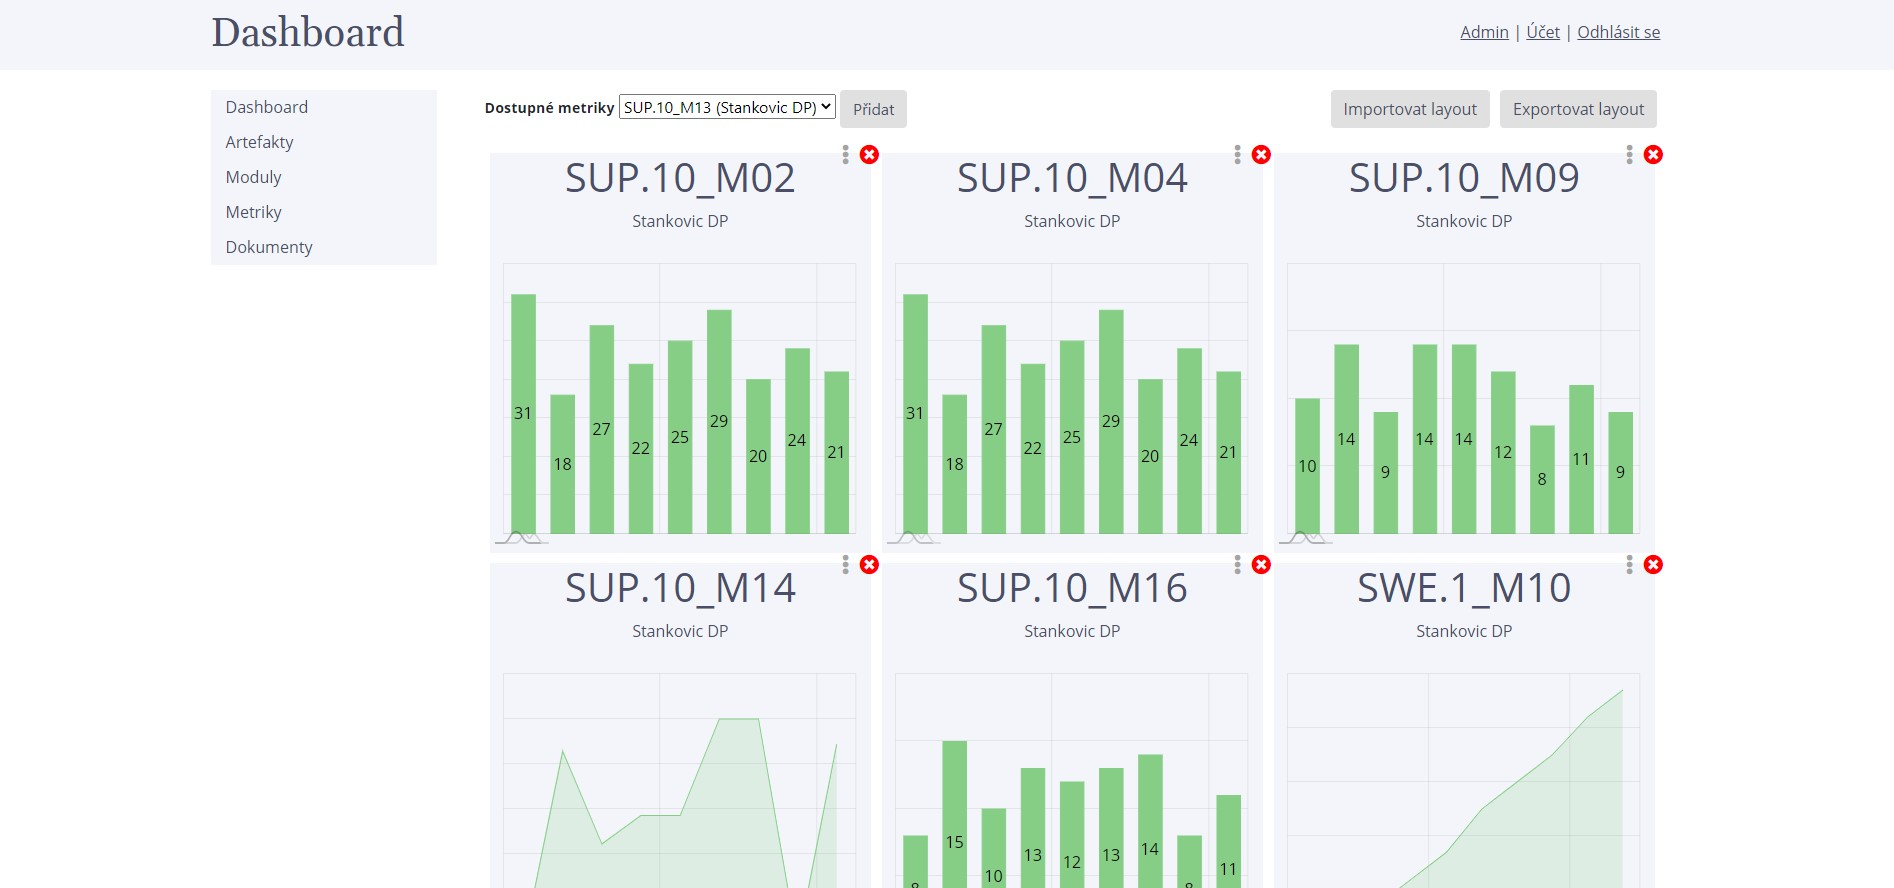
\includegraphics[width=0.8\textwidth]{Diplomka/Figures/metrics_tool/dashboard.jpg}
    \caption{Nástěnka v~uživatelské sekci nástroje}
    \label{fig:metrics_tool_dashboard}
\end{figure}
\section{Artefakty}
V~uživatelské sekci si může uživatel zobrazit například veškeré artefakty, které byly dle jednotlivých projektů staženy z~platformy IBM Jazz. Seznam artefaktů je možno nalézt na obrázku \ref{fig:metrics_tool_artifacts}. Pomocí formuláře lze také mezi jednotlivými artefakty filtrovat dle projektu.

\begin{figure}[!ht]
    \centering
    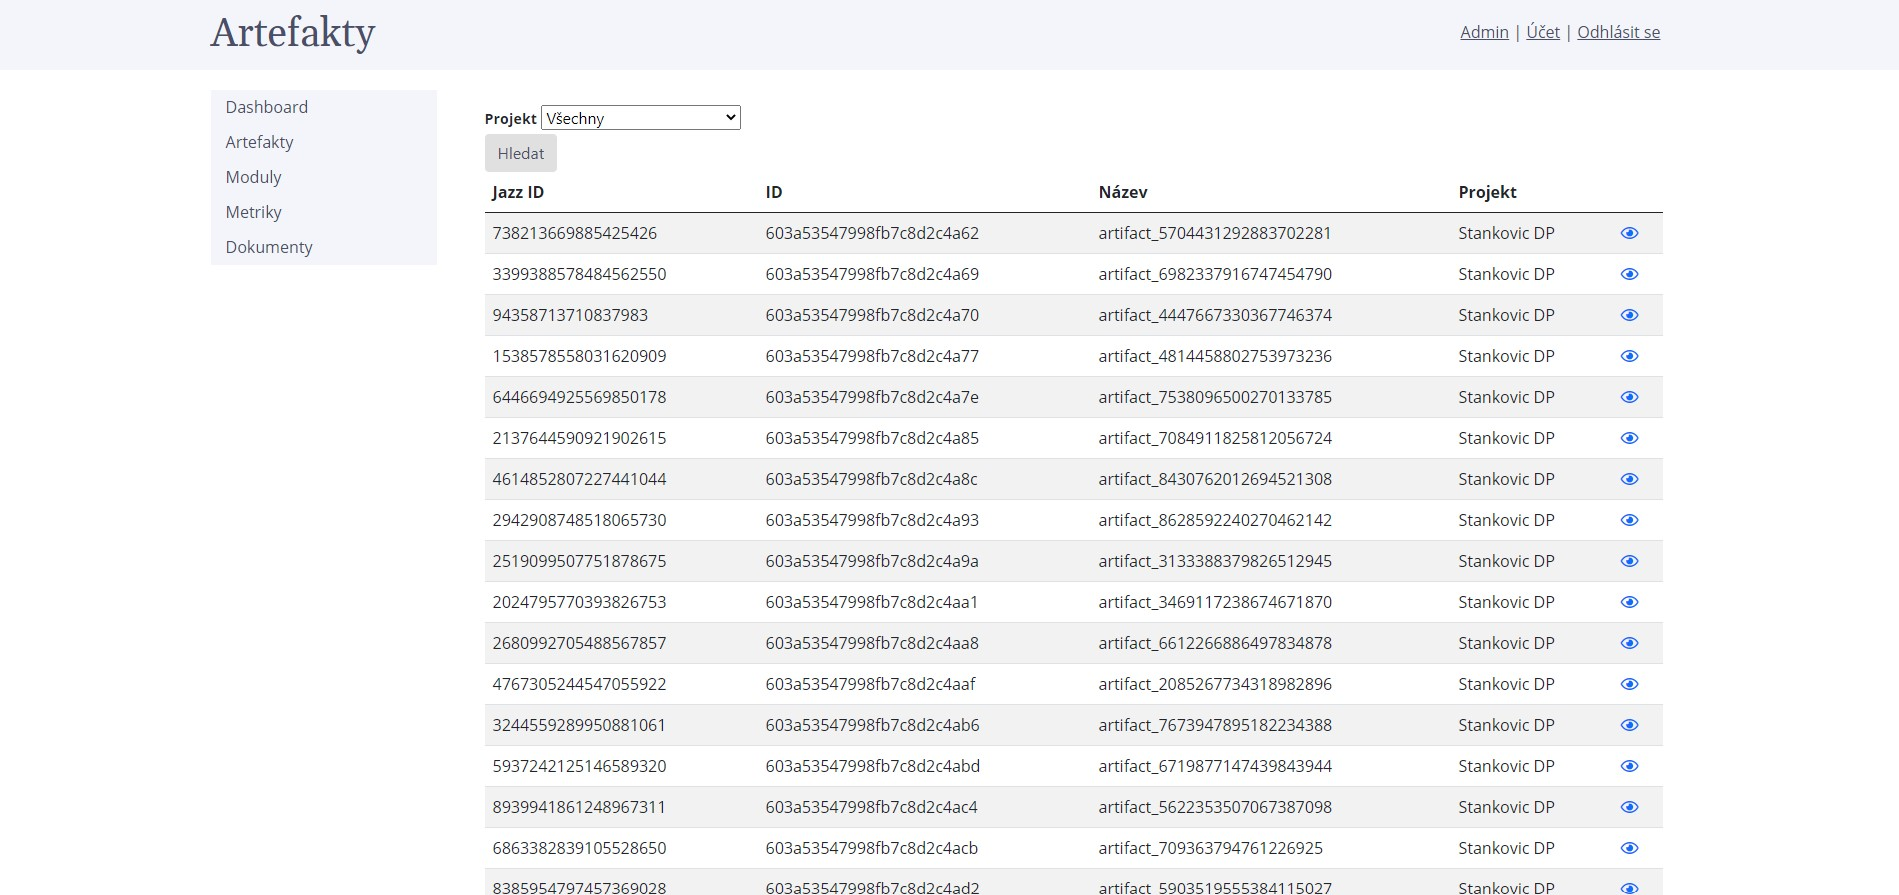
\includegraphics[width=0.9\textwidth]{Diplomka/Figures/metrics_tool/artifacts.jpg}
    \caption{Seznam artefaktů}
    \label{fig:metrics_tool_artifacts}
\end{figure}

Na obrázku \ref{fig:metrics_tool_artifacts_detail} je možno vidět detailní výpis daného artefaktu. Zde se může uživatel dozvědět veškeré informace, které jsou v~nástroji uloženy. Mezi ně patří například atributy, které jsou seřazeny dle jednotlivých dat stažení z~IBM Jazz. Kromě informací o~artefaktu se zde nachází také odkaz na původní artefakt na platformě IBM Jazz. Artefakty není možno v~nástroji upravovat, jelikož veškerá data pocházejí z~IBM Jazz.

\begin{figure}[!ht]
    \centering
    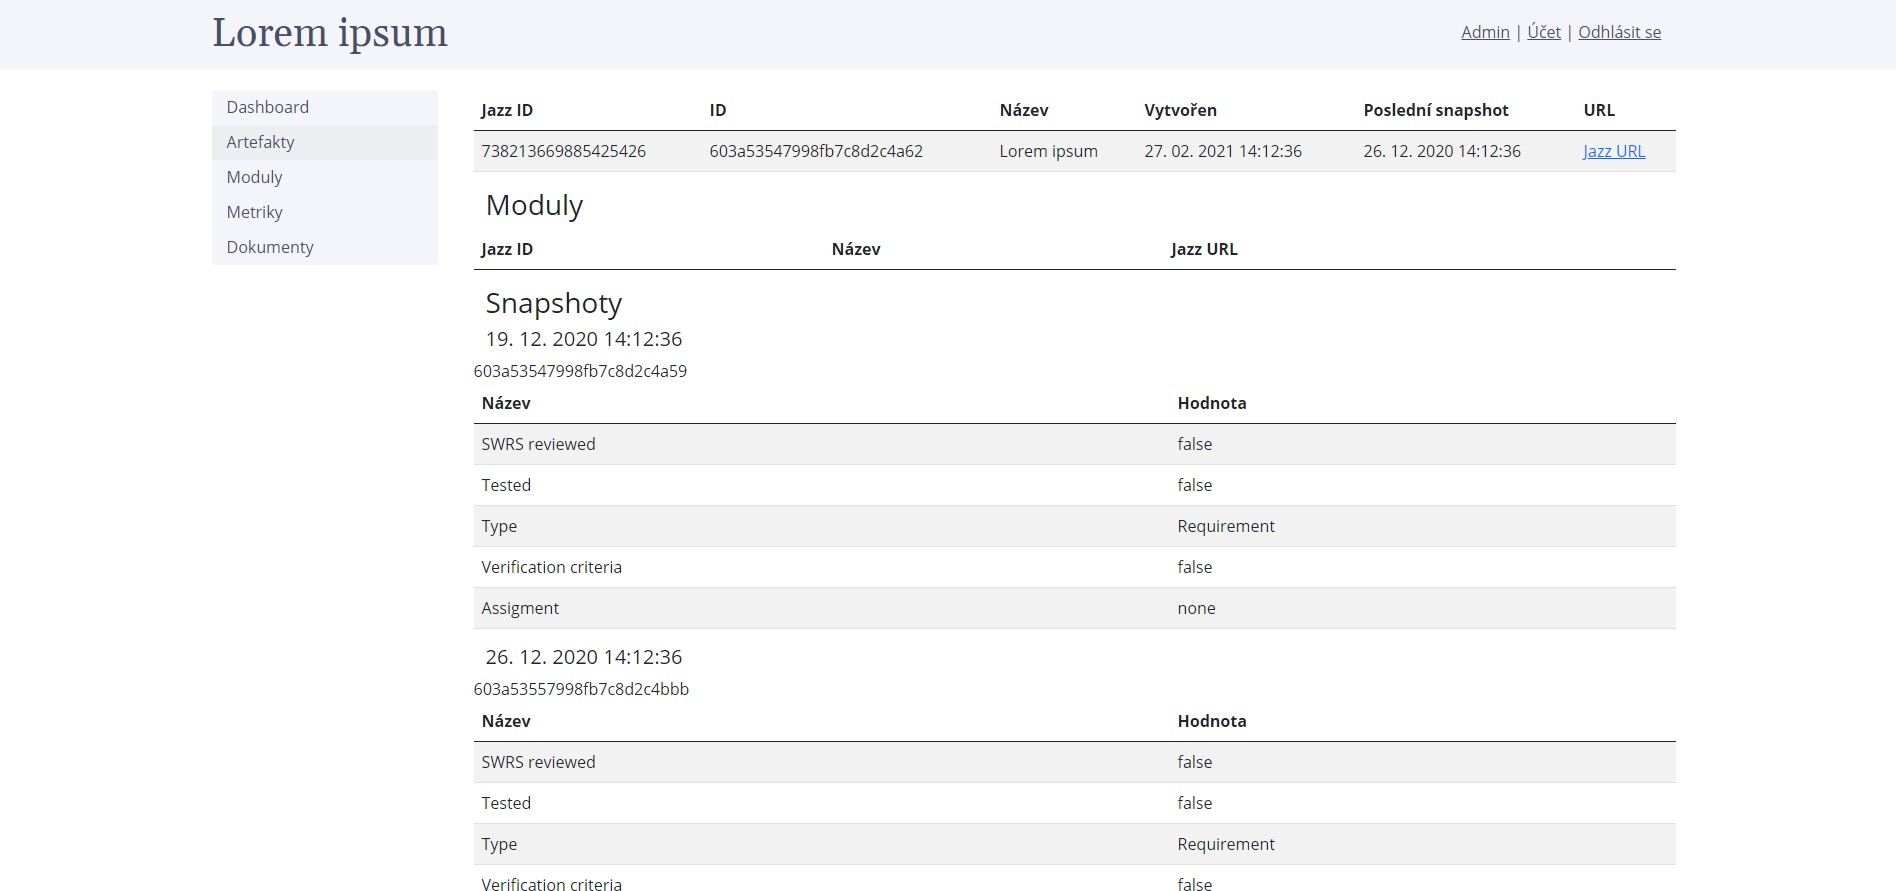
\includegraphics[width=0.9\textwidth]{Diplomka/Figures/metrics_tool/artifacts_detail.jpg}
    \caption{Detailní výpis artefaktu}
    \label{fig:metrics_tool_artifacts_detail}
\end{figure}
\section{Moduly}
Další sekcí, kterou si může uživatel pouze zobrazit a ne upravit, je seznam modulů. Moduly se stahují taktéž z~platformy IBM Jazz v~rámci stahování artefaktů, které jsou do modulů zařazeny. Výpis všech modulů dle projektu lze nalézt na obrázku \ref{fig:metrics_tool_modules}.

\begin{figure}[!ht]
    \centering
    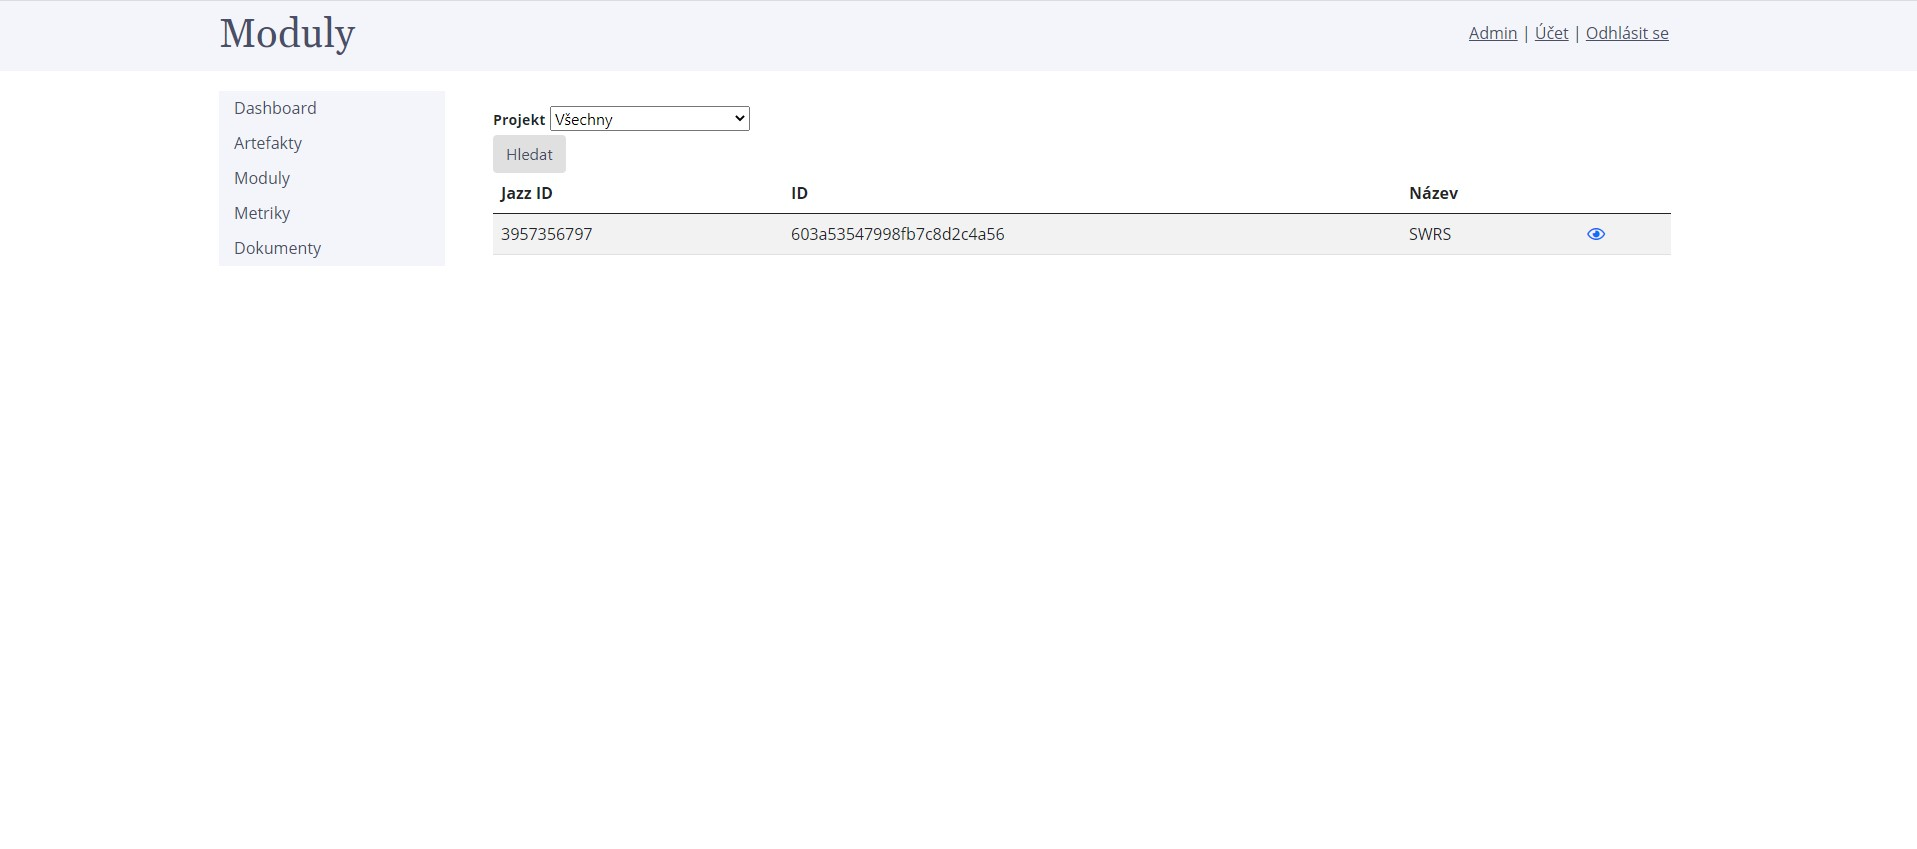
\includegraphics[width=1\textwidth]{Diplomka/Figures/metrics_tool/modules.jpg}
    \caption{Seznam modulů}
    \label{fig:metrics_tool_modules}
\end{figure}
Uživatel si stejně jako v~případě artefaktů může zobrazit také detailní výpis informací určitého modulu. Také zde se nachází odkaz na platformu IBM Jazz. Zobrazení modulu je možno vidět na obrázku \ref{fig:metrics_tool_modules_detail}.


\begin{figure}[!ht]
    \centering
    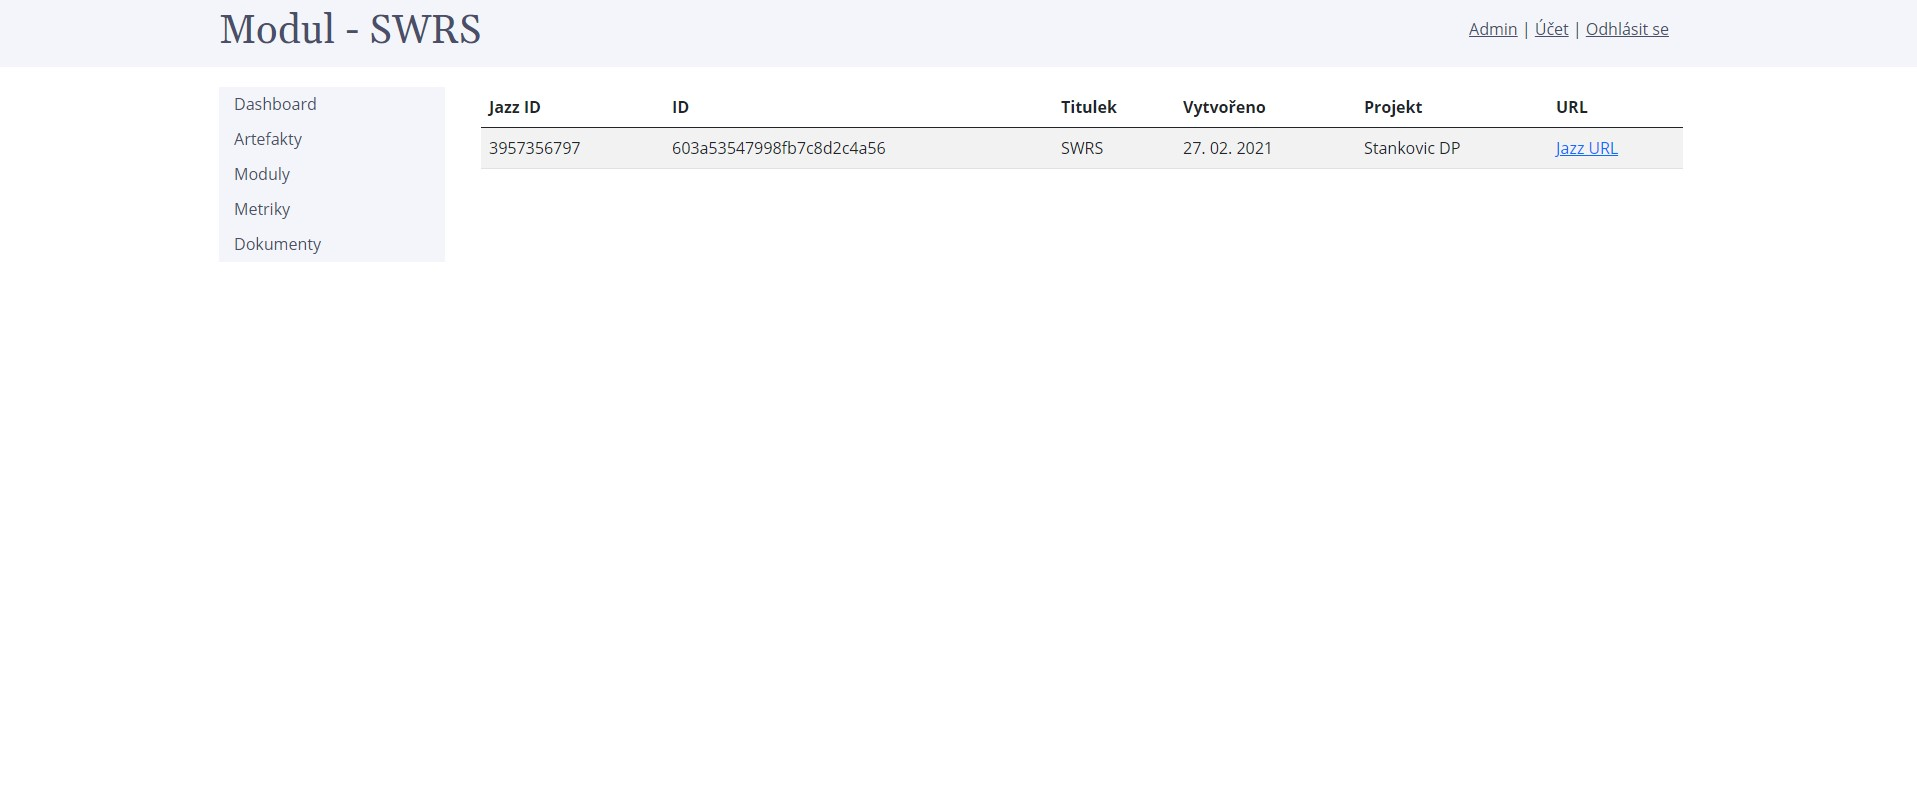
\includegraphics[width=1\textwidth]{Diplomka/Figures/metrics_tool/modules_detail.jpg}
    \caption{Detailní výpis modulu}
    \label{fig:metrics_tool_modules_detail}
\end{figure}

\newpage

\section{Metriky}

Jako další sekce v~uživatelské části nástroje se nachází metriky. Ty je možno také filtrovat dle projektu, a na rozdíl od artefaktů a modulů nepocházejí z~platformy IBM Jazz, ale jsou definovány jednotlivými uživateli. Kromě zobrazení je možno upravovat je a vytvářet z~definic metrik nové. Na obrázku \ref{fig:metrics_tool_metrics} můžeme vidět výpis všech metrik dle projektu. Dále lze vidět na obrázku \ref{fig:metrics_tool_metrics_detail} zobrazení metriky včetně grafu, tabulky a podmínek a na obrázku \ref{fig:metrics_tool_metrics_edit} úpravu existující metriky.

\begin{figure}[!ht]
    \centering
    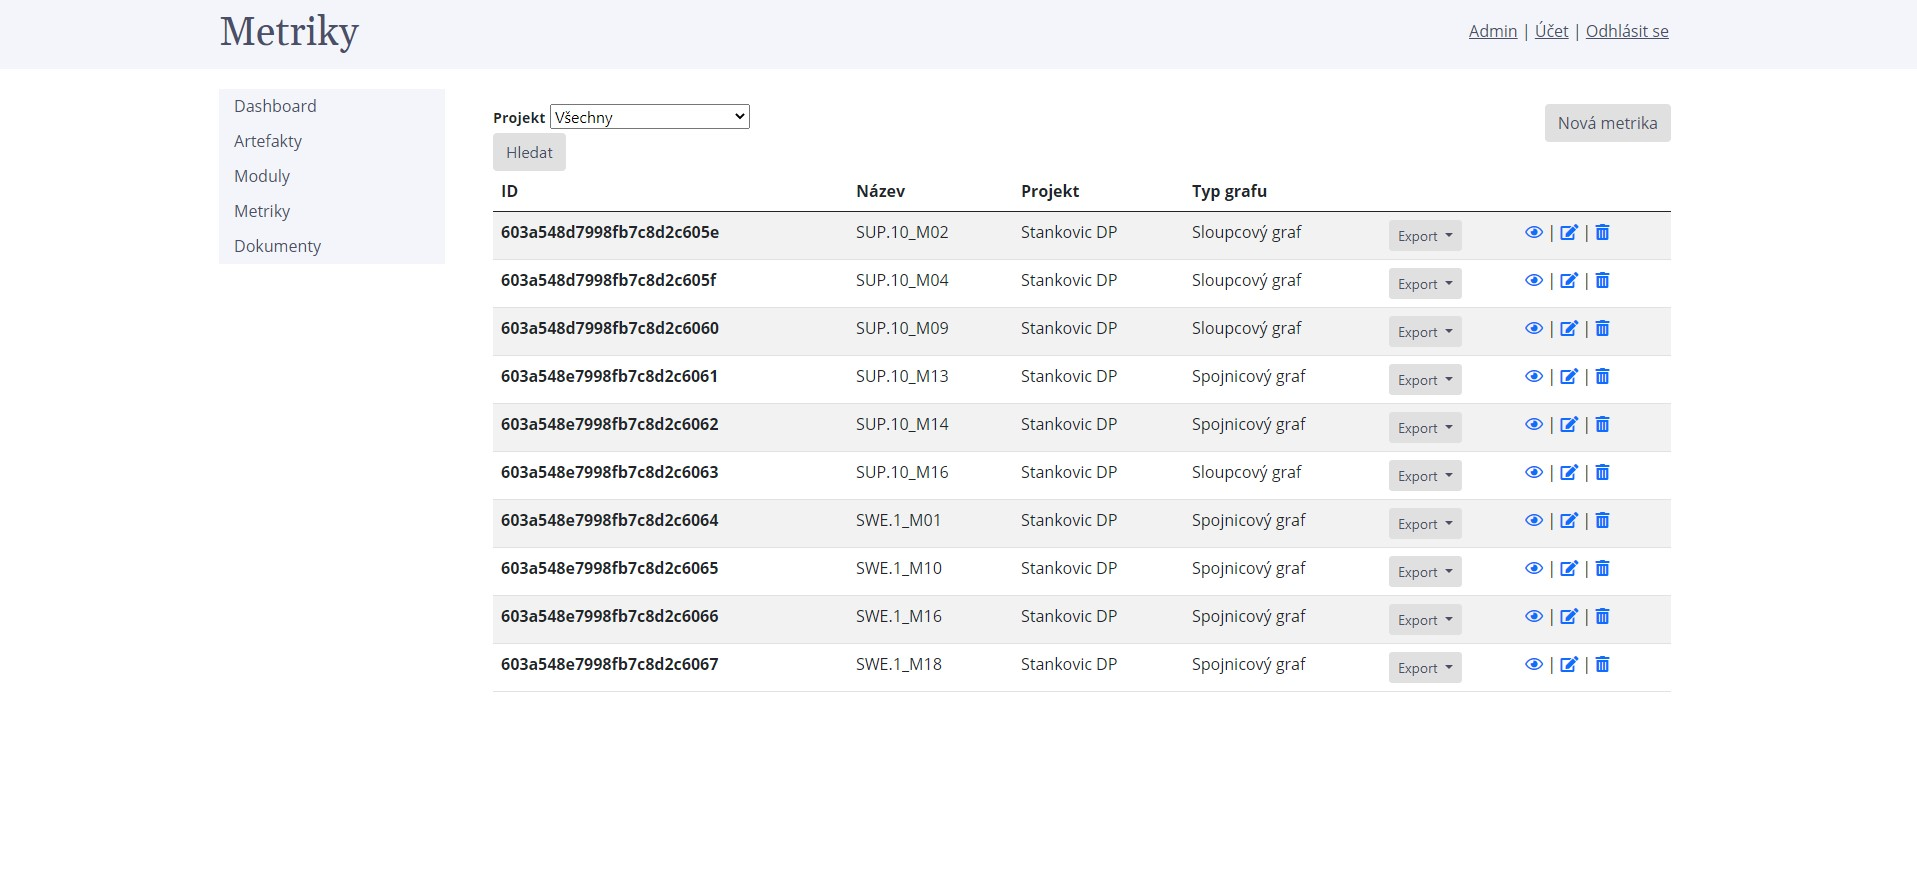
\includegraphics[width=1\textwidth]{Diplomka/Figures/metrics_tool/metrics.jpg}
    \caption{Seznam metrik}
    \label{fig:metrics_tool_metrics}
\end{figure}

\begin{figure}[!ht]
    \centering
    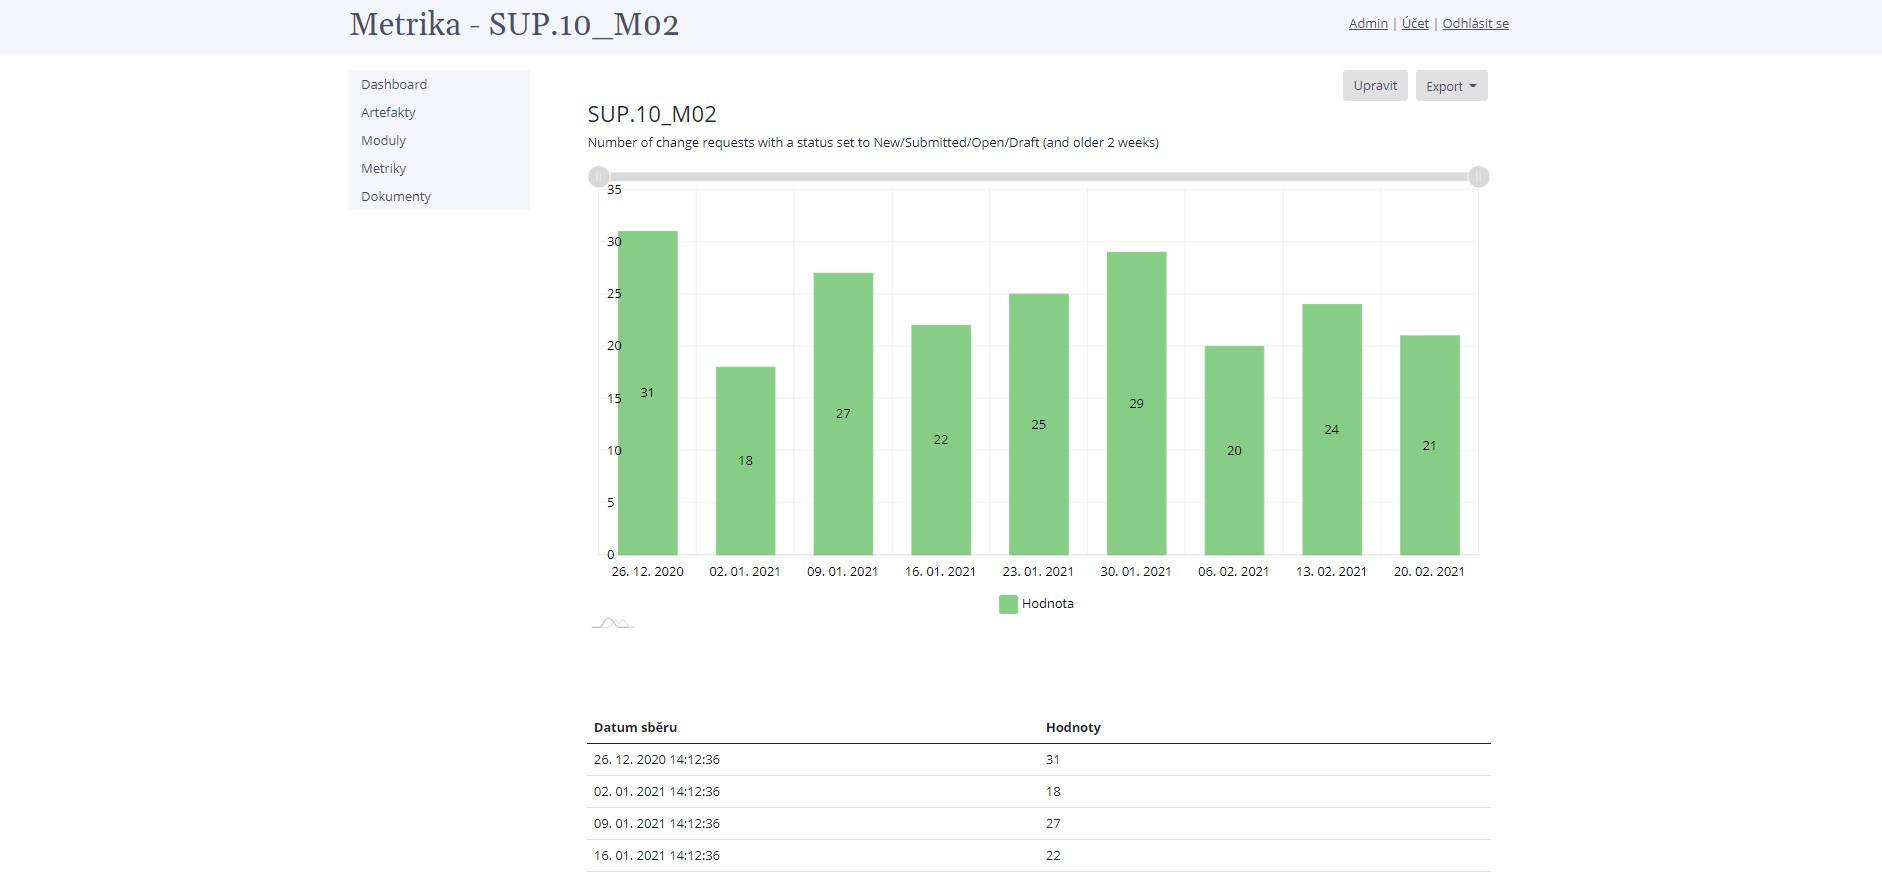
\includegraphics[width=1\textwidth]{Diplomka/Figures/metrics_tool/metrics_detail.jpg}
    \caption{Zobrazení detailu metriky}
    \label{fig:metrics_tool_metrics_detail}
\end{figure}


\begin{figure}[!ht]
    \centering
    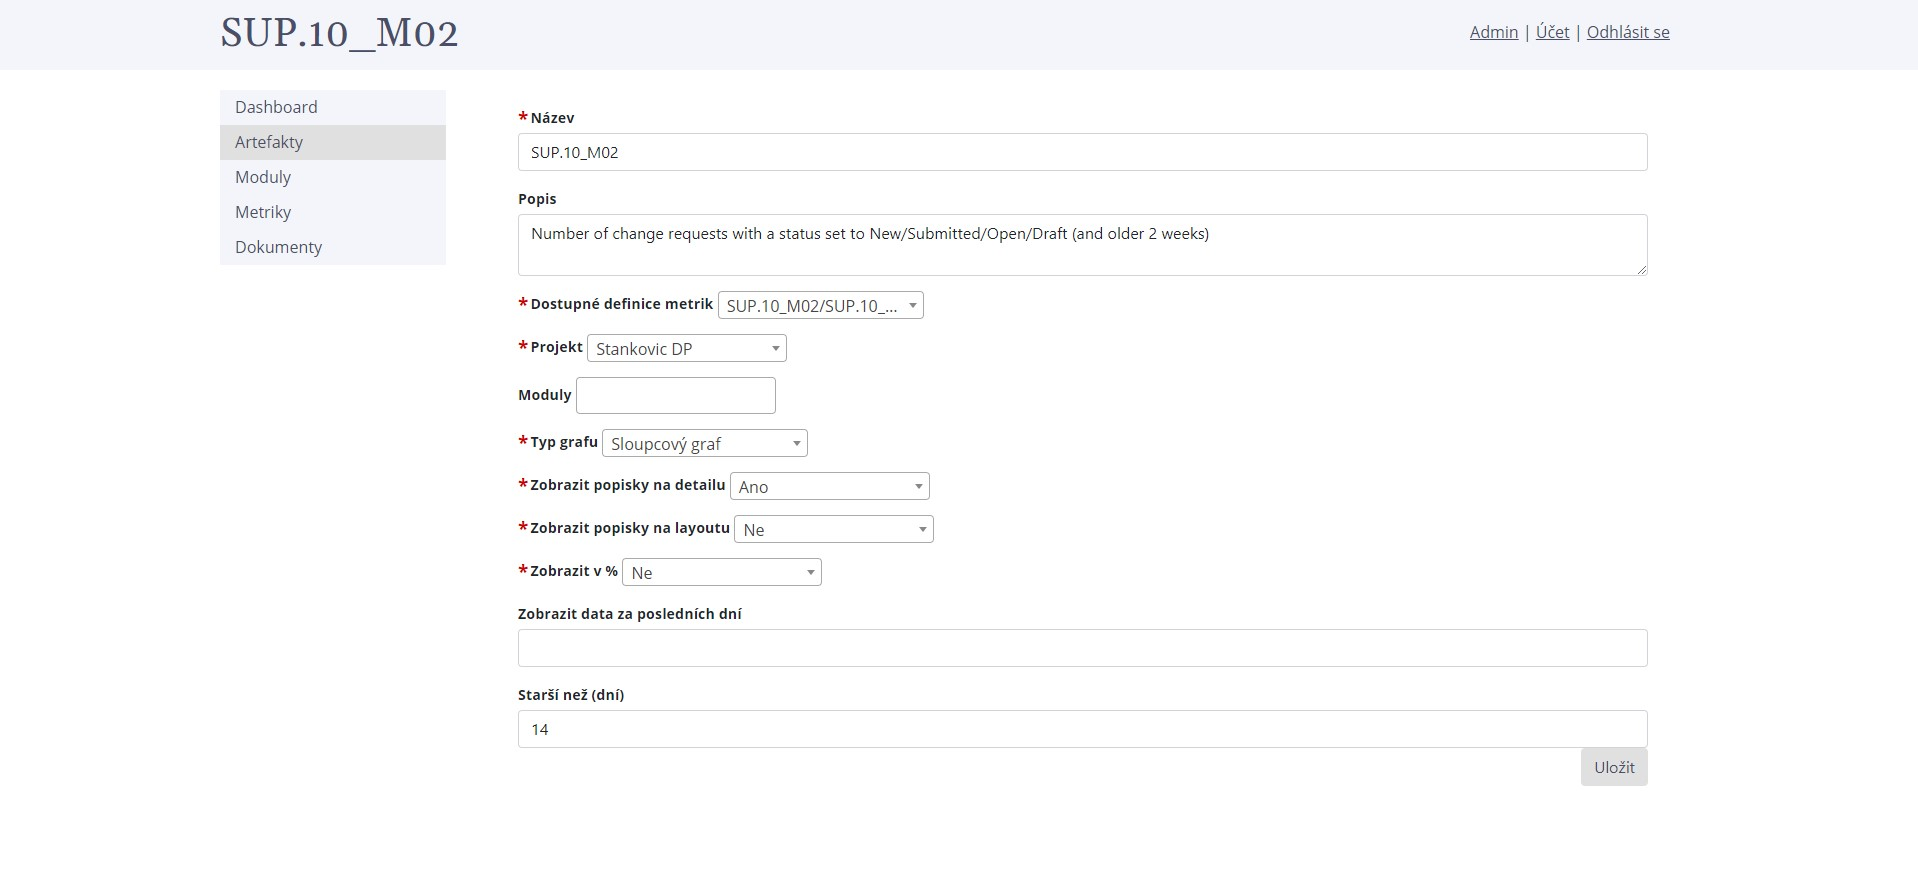
\includegraphics[width=1\textwidth]{Diplomka/Figures/metrics_tool/metrics_edit.jpg}
    \caption{Úprava metriky}
    \label{fig:metrics_tool_metrics_edit}
\end{figure}
\section{Dokumenty}
Jednou z~posledních důležitých funkcionalit v~rámci nástroje jsou dokumenty pro reporty. Ty slouží jako dynamické a statické dokumenty obsahující text a metriky buď v~podobě tabulky, nebo grafu. Dokumenty si lze zobrazit v~dynamické podobě přímo v~nástroji, případně stáhnout v~požadovaném formátu. Mezi možné formáty patří například Word a PowerPoint, přičemž je možné rozšíření na HTML a PDF. Na obrázku \ref{fig:metrics_tool_documents} můžeme vidět výpis všech dynamických dokumentů dle projektu, dále na obrázku \ref{fig:metrics_tool_documents_detail} detailní výpis dynamického dokumentu, který se mění dle stahovaných dat, a na obrázku \ref{fig:metrics_tool_documents_edit} můžeme vidět úpravu dokumentu. Při úpravě si může uživatel dokument libovolně skládat pomocí bloků. 

\begin{figure}[!ht]
    \centering
    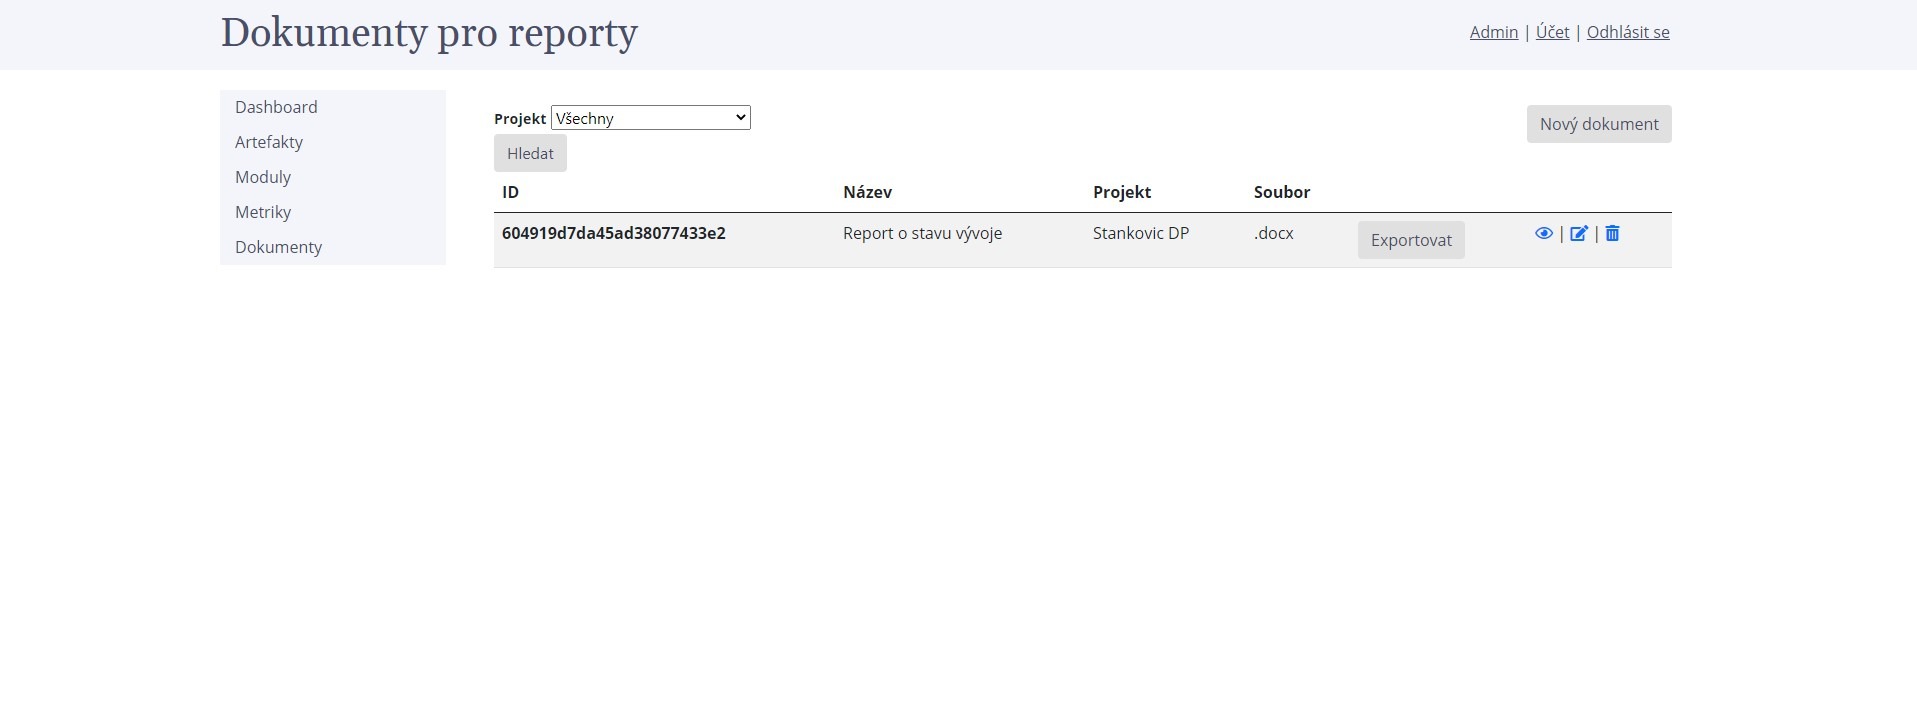
\includegraphics[width=1\textwidth]{Diplomka/Figures/metrics_tool/documents.jpg}
    \caption{Seznam dokumentů}
    \label{fig:metrics_tool_documents}
\end{figure}

\begin{figure}[!ht]
    \centering
    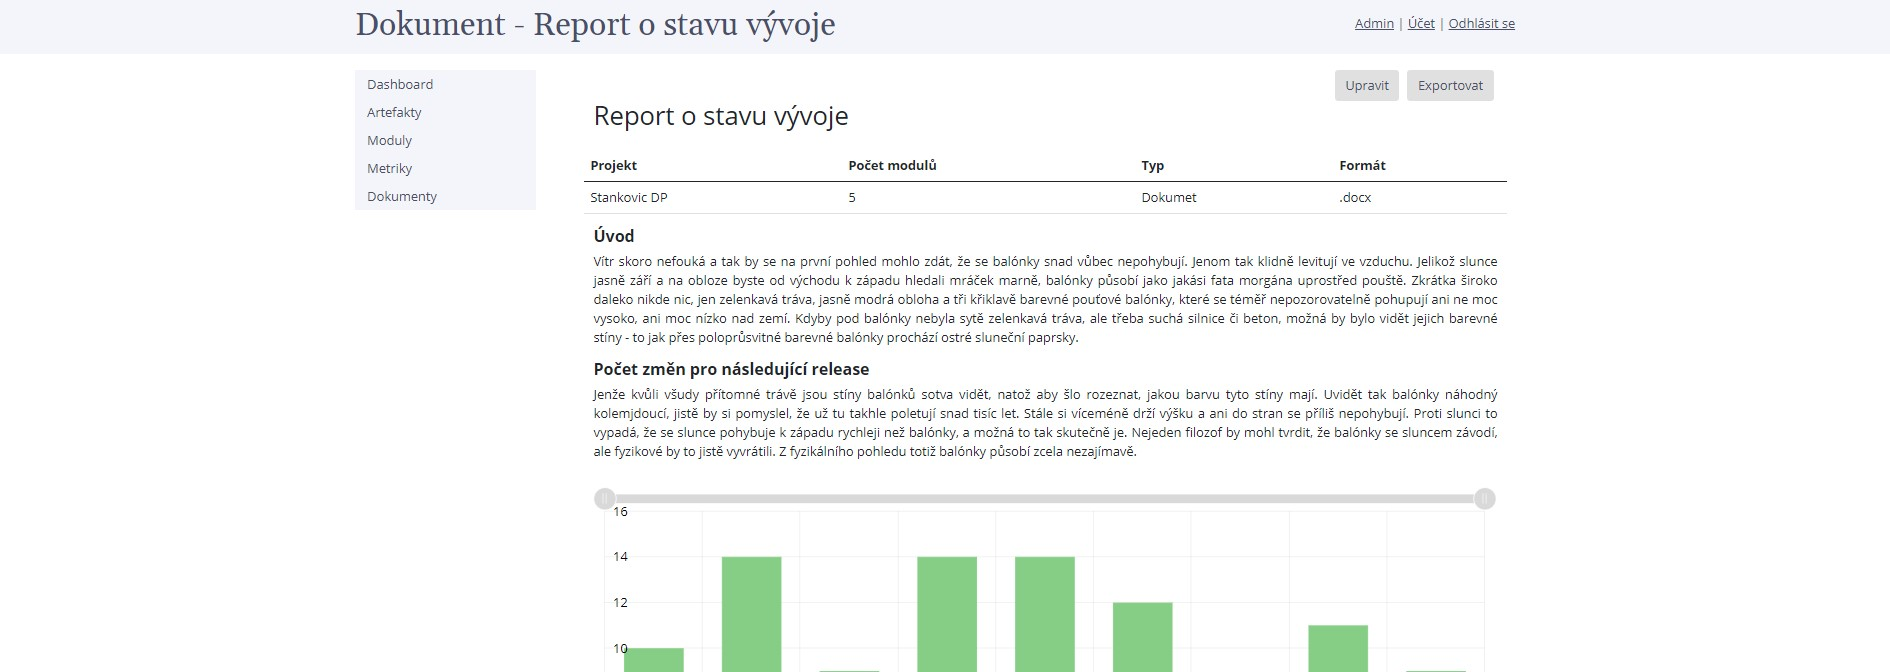
\includegraphics[width=1\textwidth]{Diplomka/Figures/metrics_tool/documents_detail.jpg}
    \caption{Zobrazení detailu dynamcikého dokumentu}
    \label{fig:metrics_tool_documents_detail}
\end{figure}


\begin{figure}[!ht]
    \centering
    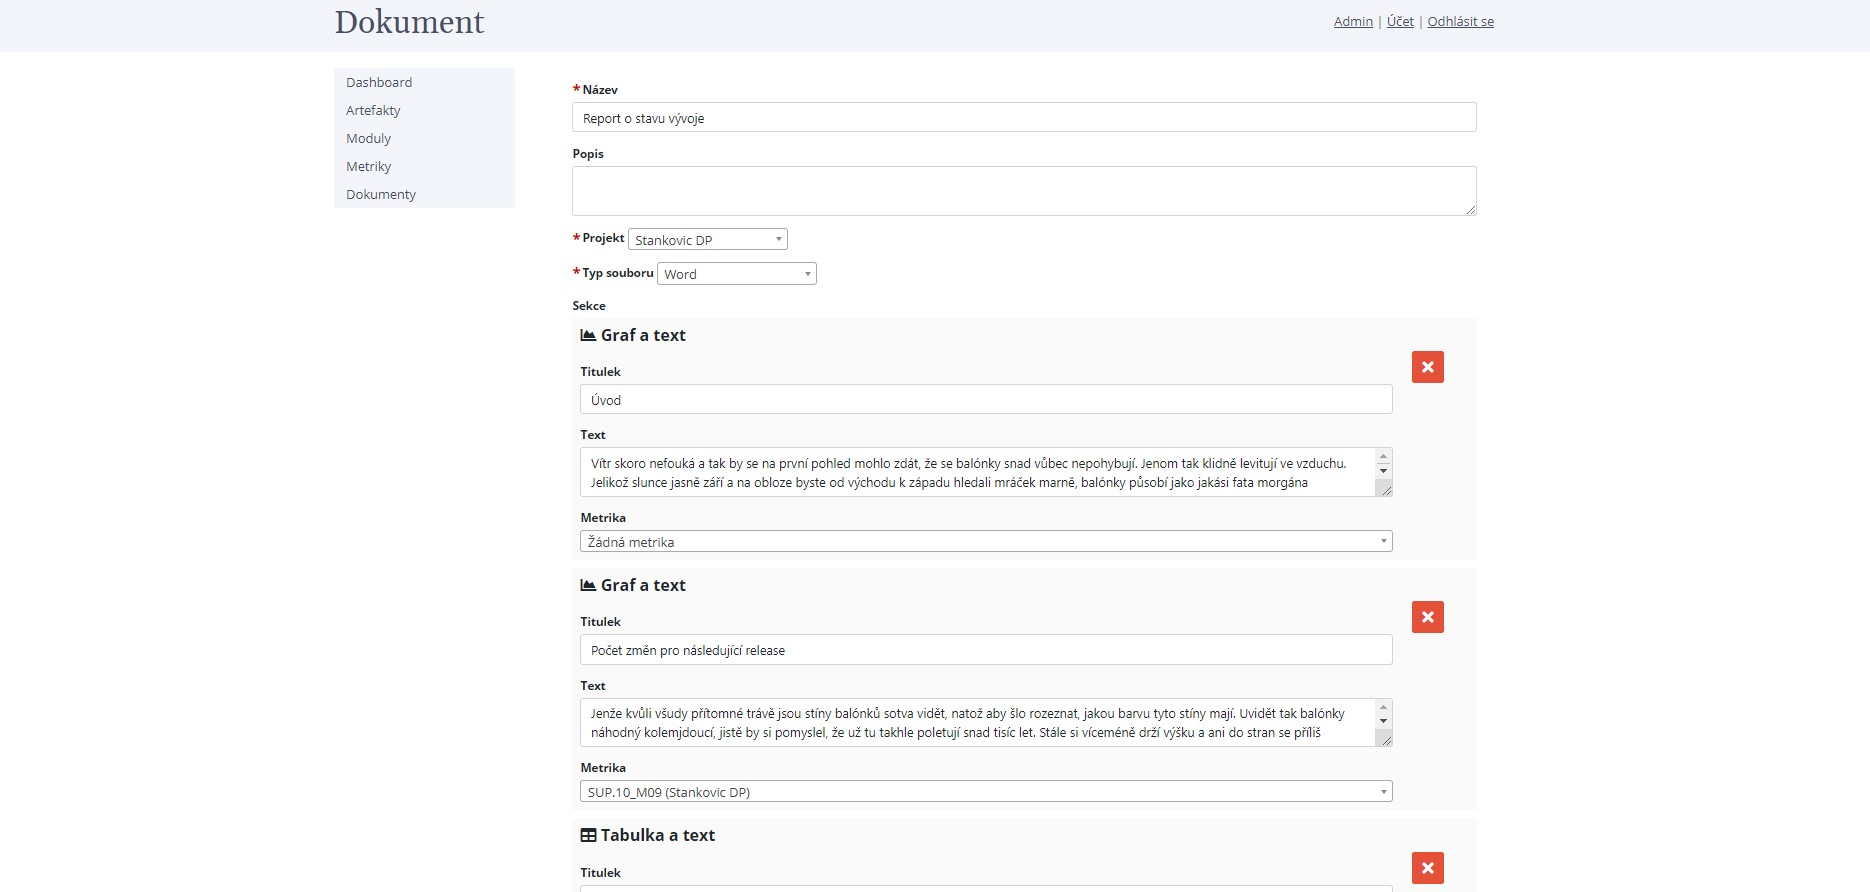
\includegraphics[width=1\textwidth]{Diplomka/Figures/metrics_tool/documents_edit.jpg}
    \caption{Úprava dokumentu}
    \label{fig:metrics_tool_documents_edit}
\end{figure}
\newpage
\section{Projekty}

V~rámci administrace může administrátor vytvářet a upravovat projekty, které propojí s~platformou IBM Jazz pomocí identifikátoru daného projektu. Výpis projektů v~administraci lze nalézt na obrázku \ref{fig:metrics_tool_admin_projects}.


\begin{figure}[!ht]
    \centering
    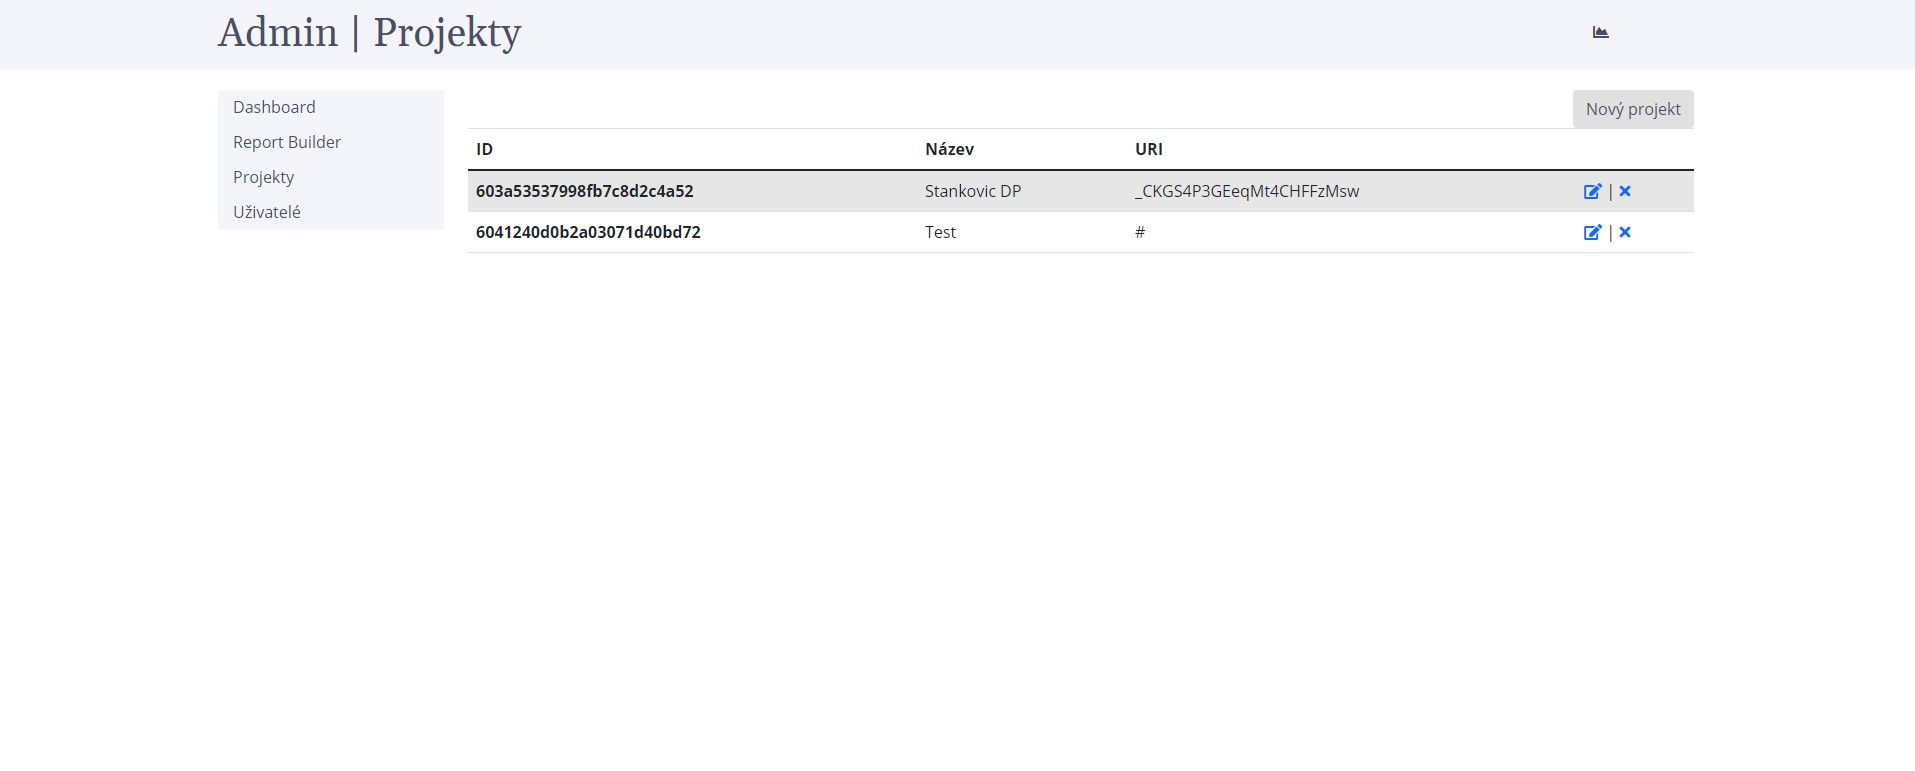
\includegraphics[width=1\textwidth]{Diplomka/Figures/metrics_tool/admin_projects.jpg}
    \caption{Výpis vytvořených projektů}
    \label{fig:metrics_tool_admin_projects}
\end{figure}
\newpage
\section{Definice metrik}
Jednou z~nejdůležitějších části nástroje je možnost vytvářet v~administraci definice metrik, které slouží pro následné vytváření metrik pro jednotlivé metriky. Definici metriky si lze představit jako seznam podmínek, které jsou nutné pro vytvoření a vygenerování metriky. Definice je zcela nezávislá na typu grafu nebo projektu. Seznam vytvořených definic je možno vidět na obrázku \ref{fig:admin_report_builder}. Pomocí vícekrokového formuláře může administrátor nastavit základní údaje definice a vybrat podmínky pro definici metriky. Podmínky jsou vytvářeny z~dat stahovaných z~platformy IBM Jazz. Formulář lze nalézt na obrázku \ref{fig:admin_report_builder_first_first} a \ref{fig:admin_report_builder_second}.

\begin{figure}[!ht]
    \centering
    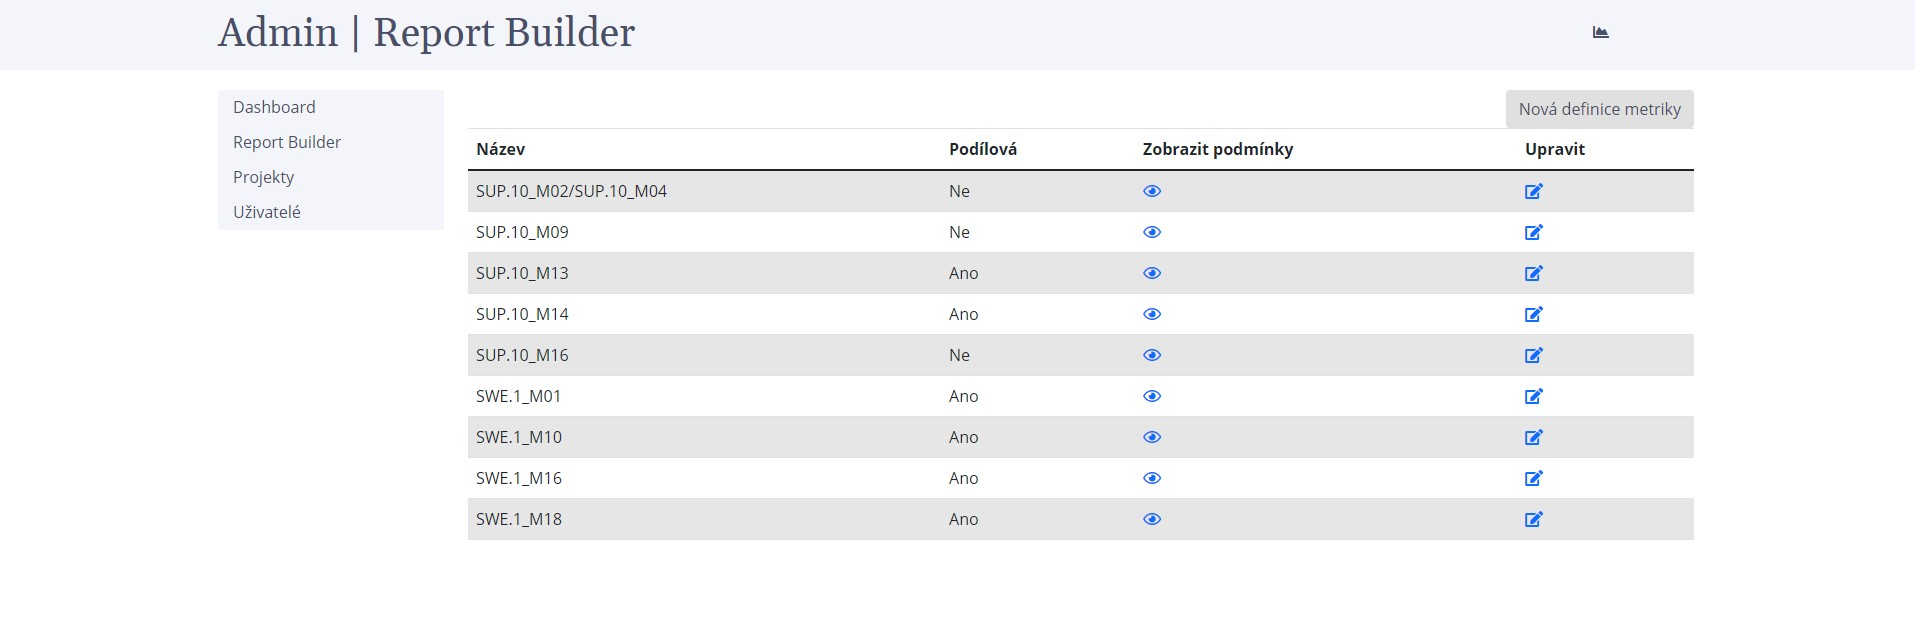
\includegraphics[width=1\textwidth]{Diplomka/Figures/metrics_tool/admin_report_builder.jpg}
    \caption{Výpis vytvořených definic metrik}
    \label{fig:admin_report_builder}
\end{figure}

\begin{figure}[!ht]
    \centering
    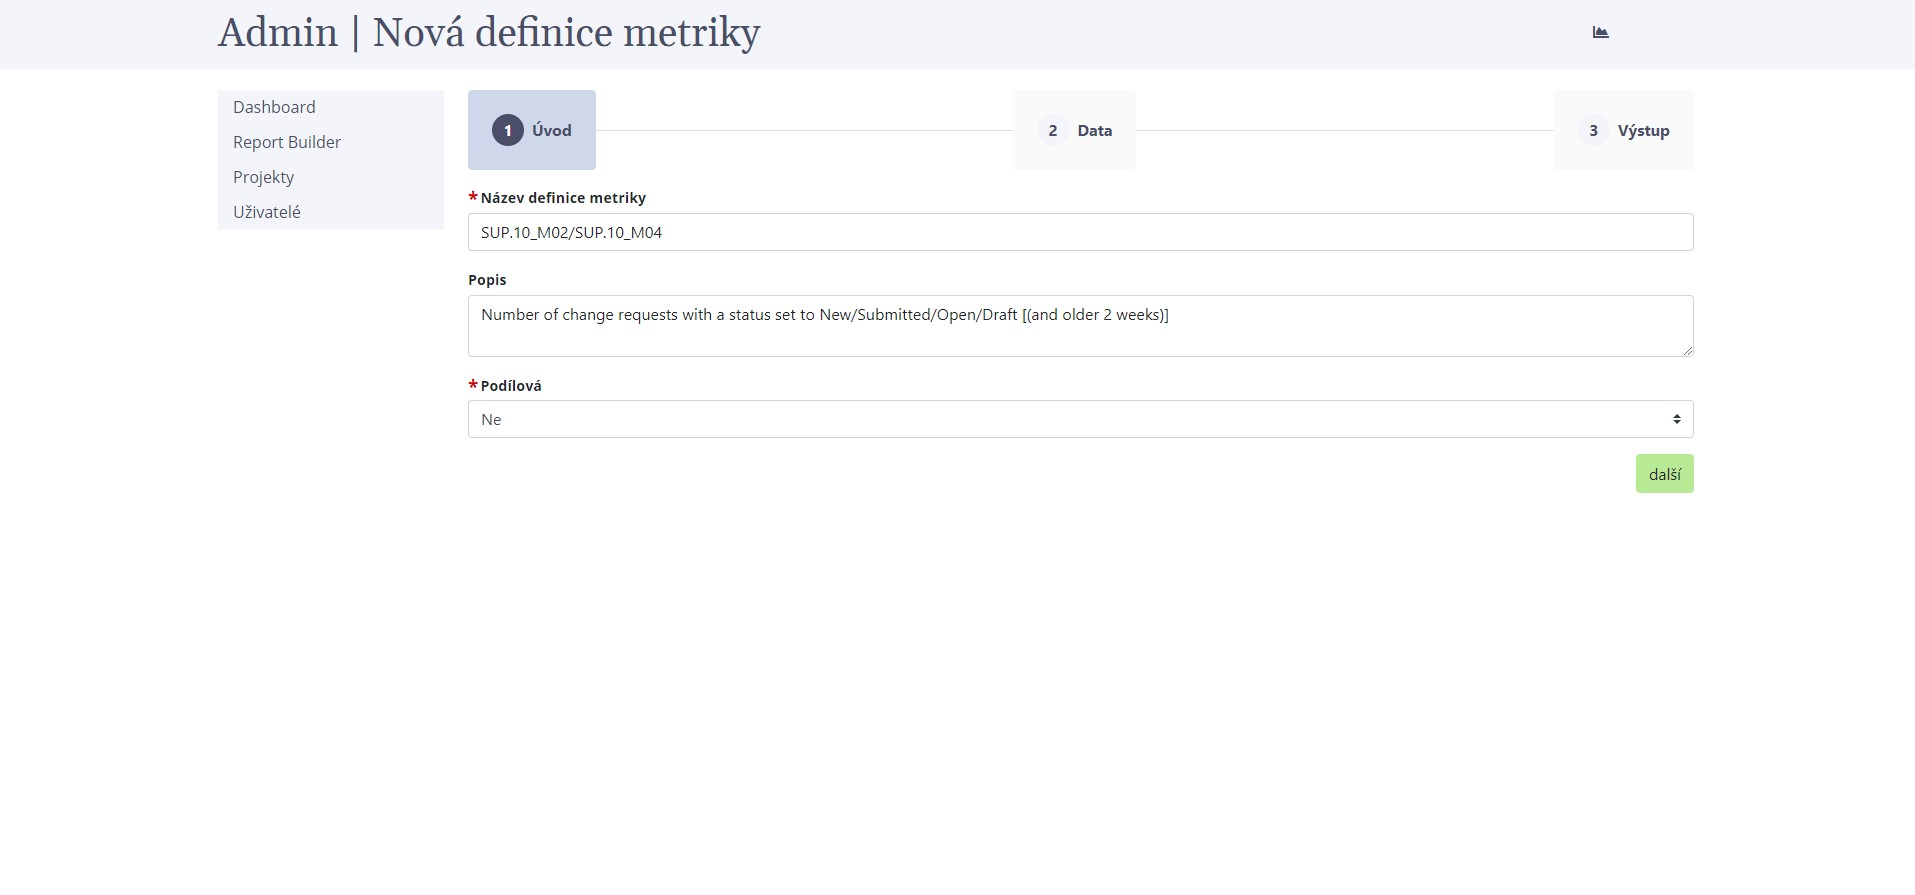
\includegraphics[width=1\textwidth]{Diplomka/Figures/metrics_tool/admin_report_builder_first.jpg}
    \caption{Základní nastavení definice metriky}
    \label{fig:admin_report_builder_first_first}
\end{figure}

\begin{figure}[!ht]
    \centering
    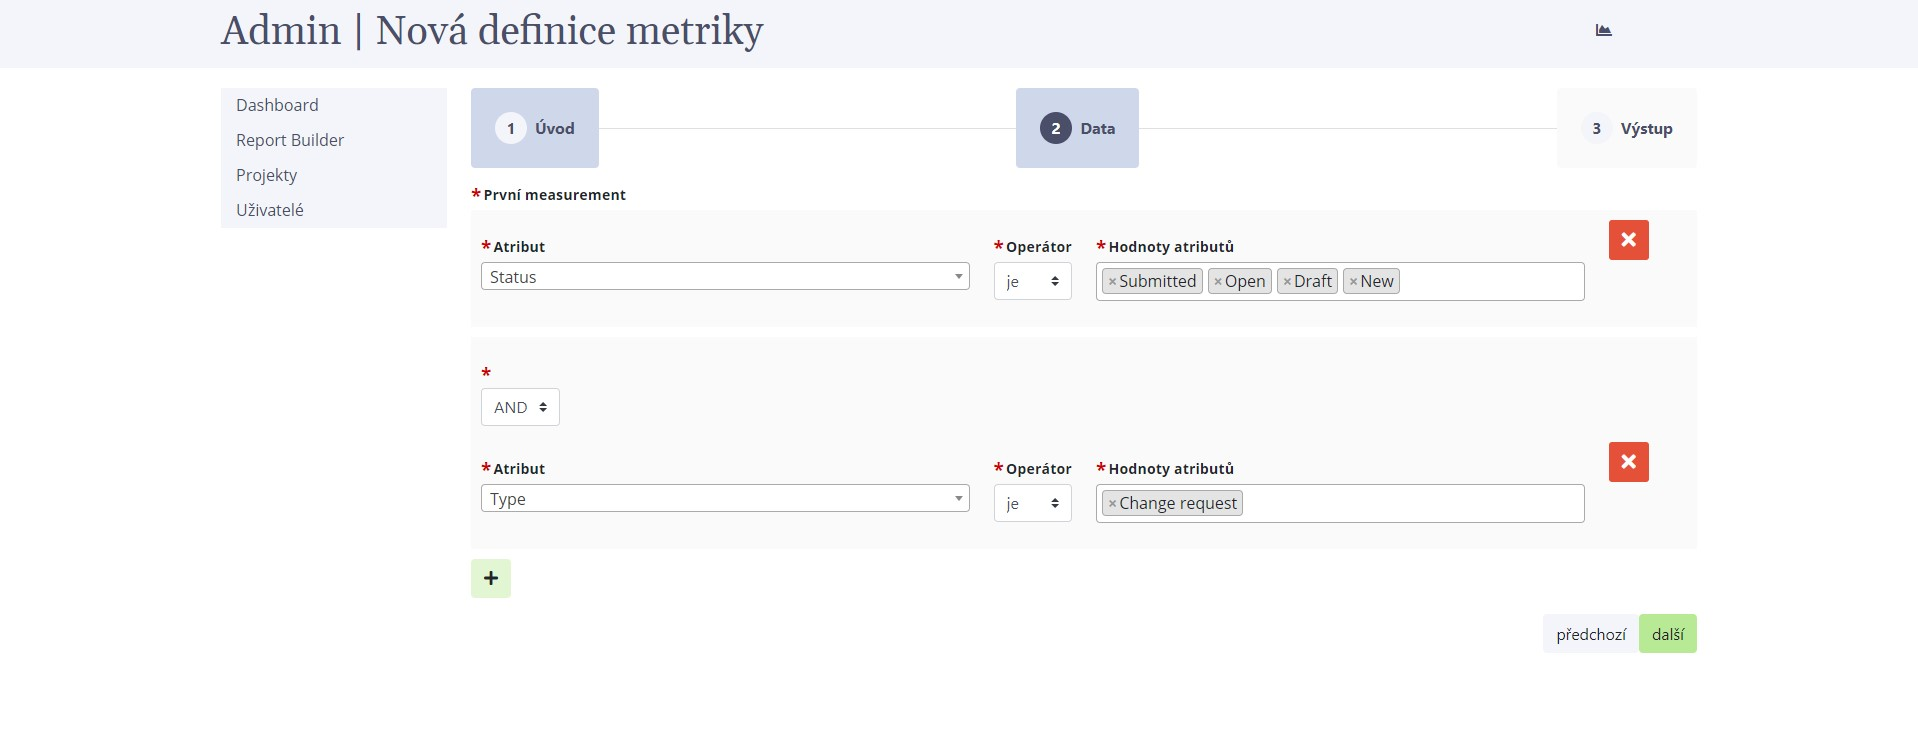
\includegraphics[width=1\textwidth]{Diplomka/Figures/metrics_tool/admin_report_builder_second.jpg}
    \caption{Zvolení podmínek pro definici metriky}
    \label{fig:admin_report_builder_second}
\end{figure}
\end{document}
